\documentclass[a4paper, 11pt]{article}
\usepackage[a4paper, margin=2cm]{geometry}
\usepackage[utf8]{inputenc}
\usepackage[T1]{fontenc}
\usepackage{microtype}
\usepackage{times}
\usepackage[czech]{babel}
\usepackage[unicode,hidelinks]{hyperref}
\usepackage{parskip}
\usepackage{graphicx}
\usepackage{grffile}
\usepackage{caption}

\usepackage{enumitem}
\setlist{nosep,after=\vspace{\medskipamount}}
\setlist[description]{font={\itshape},labelsep=0.3em}
\usepackage{parskip}
\usepackage{setspace}
\usepackage{xcolor}
\usepackage{dsfont}
\usepackage{amsmath}

\newcommand{\tcmd}[1]{\texttt{#1}}
\newcommand{\lpath}[1]{\texttt{#1}}
\newcommand{\ttrue}{\texttt{true}}
\newcommand{\tfalse}{\texttt{false}}

\title{IOS -- Operační systémy}
\date{}

\begin{document}
%%
%%  TITULNI STRANA
%%
\begin{titlepage}

\begin{center}
\LARGE
\textsc{\Huge Vysoké učení technické v Brně}\\
\textsc{\huge Fakulta informačních technologií}\\
\vspace{\stretch{0.382}}
the Little Book of IOS\\[0.4em]
{\Huge Poznámky z přednášek}
\vspace{\stretch{0.618}}
\end{center}
{\Large 2019/2020 \footnotesize(PDF z \today) \hfill \Large Corse\footnotesize\,\&\,LeO}

\end{titlepage}

%%
%% OBSAH
%%

\tableofcontents

%%
%%  TEXT
%%

\newpage

\setstretch{1.1}
\textbf{Preambule}

Dokument je dělen dle přednášek a toho, co se probíralo na přednáškách IOS (ak. r. 2019/2020). Tedy každá hlavní kategorie značí číslo přednášky, podkategorie značí probírané téma a případně jsou použity i pod\-pod\-ka\-te\-go\-ri\-e pro rozdělení velkých témat do více úseků.

Je docela možné, že spousta věcí bude pouze přepisem obsahu prezentace, nicméně takto celý dokument (ani jediný řádek, až na výjimky, jako je třeba deadlock) zpracováván nebyl. Dokument byl zpracován za pomoci záznamů přednášek, a to tak, abych dané téma či látku dostatečně pochopil a zároveň bylo zajištěno nějakým způsobem, aby dané vysvětlení nebylo až moc polopatické a stačilo např. ke zkoušce.
 
Někdy pro pochopení dané látky byly vhodné obrázky, někde byly i nutností (např. princip souborových systémů). Také jsou obrázky použity pro pseudokódy, protože nějaké normální zpracování kódu v \LaTeX u by trvalo zbytečně dlouho. Všechny obrázky (i pseudokódy) byly použity z různých prezentací IOS. Moje rozhodně nejsou -- pod popiskem každého obrázku je tak zmínka o tom, odkud daný obrázek pochází.
 
Co se týče pochopení obsahu, bylo by dobré spolu před čtením jakékoli kapitoly (=přednášky) navštívit danou přednášku nebo si ji alespoň pustit ze záznamu. Bez toho je možné, že některé věci nebude možné pochopit. 

\newpage

\section{} \label{start-of-doc}
\textbf{První přednáška:} Úvod do předmětu, přehled operačních systémů, základní pojmy, jádro operačního systému a jejich typy, historie vývoje operačních systémů, přehled technického vybavení, klasifikace počítačů, operačních systémů, hlavní směry ve vývoji operačního systému.

\subsection{Úvod, přehled operačních systémů}
Operační systém je významnou částí výpočetních systémů; ty zahrnují:
\begin{itemize}
    \item hardware, 
    \item operační systém,
    \item uživatelské aplikační programy,
    \item uživatele.
\end{itemize}

Přehled některých OS:
\begin{itemize}
    \item GNU/Linux 
    \begin{itemize}
        \item Debian -- Ubuntu 
        \item Red Hat: RHEL, Fedora, CentOS 
        \item SuSE 
        \item Gentoo
        \item Arch Linux
        \item Slackware (nejstarší live distribuce Linuxu)
    \end{itemize}
    \item BSD 
    \begin{itemize}
        \item FreeBSD, OpenBSD 
    \end{itemize}
    \item GNU
    \begin{itemize}
        \item zn. GNU Is Not Unix
    \end{itemize}
    \item MS Windows 
    \item Mac OS X
    \begin{itemize}
        \item jádro XNU = X is Not Unix
    \end{itemize}
    \item Android, iOS
    \item Minix
    \begin{itemize}
        \item používá Intel ve svých čipech
    \end{itemize}
\end{itemize}
\newpage

\subsection{Základní pojmy}
Operační systém je program (resp. kolekce programů), která vytváří spojující mezivrstvu mezi hardware operačního systému, uživateli a jejich uživatelskými aplikačními programy. OS dále spotřebovává zdroje, jako jsou paměť nebo čas CPU.
(TLDR: SW spojující hardware, uživatele a programy.)

\textbf{Cíle OS:}
\begin{itemize}
    \item maximální využití zdrojů počítače -- drahé počítače, levnější pracovní síla (dříve)
    \item jednoduchost použití počítačů -- levné počítače, drahá pracovní síla (dnes převažuje)
\end{itemize}

\textbf{Základní role OS:}
\begin{itemize}
    \item správce prostředků
        \begin{itemize}
            \item paměť, procesor, periferie
             \item dovoluje sdílet prostředky efektivně a bezpečně
        \end{itemize}
    \item tvůrce prostředí pro uživatele a jejich aplikační programy
        \begin{itemize}
            \item vytváření abstrakcí, virtuálních objektů (resp. poskytuje standardní rozhraní, které zjednodušuje přenositelnost aplikací a zaučení uživatelů)
            \item abstrakce jsou například: proces, program, soubor
            \item problémy abstrakcí: menší efektivita a nepřístupné některé nízkoúrovňové operace
        \end{itemize}
\end{itemize}

\textbf{OS zahrnuje:}
\begin{itemize}
    \item jádro (kernel),
    \item systémové knihovny a utility (= systémové aplikační programy),
    \item textové (Shell) či grafické uživatelské rozhraní (X Window System).
\end{itemize}

Přesná definice, co vše OS zahrnuje, neexistuje. Různé firmy a komunity to chápou různě. (GNU to chápe např. jako projekt svobodného OS zahrnující jádro, utility, GUI, TUI, vývojové prostředky a knihovny, \ldots)

\subsection*{Definice:} \label{procesy} \label{soubory}
\begin{description}
\item[proces] je aktivita řízená programem (podrobněji se jim věnujeme od \ref{procesy-detailed})
\item[program] je předpis, návod na nějakou činnost zakódovaný vhodným způsobem
\item[soubor] je kolekce záznamů sloužící primárně jako základní jednotka pro ukládání dat na vnějších paměťových médiích
\item[adresář] je kolekce souborů
\end{description}

\newpage
\subsection{Jádro operačního systému}
Jedná se o nejnižší a nejzákladnější část OS. Zavádí se jako první a běží po celou dobu běhu počítačového systému (tzv. reaktivní systém, spíš než transformační). Navazuje přímo na hardware (případně virtualizovaný HW) a pro uživatele a uživatelské aplikace jej zcela zapouzdřuje.

\textbf{Běží v privilegovaném režimu:}
\begin{itemize}
    \item je možné měnit obsah registru HW, je možné zadávat příkazy HW (není možné v~uživatelském režimu)
    \item musí být podporováno v HW
\end{itemize}

\textbf{Jádro (obecně) zajišťuje:}
\begin{itemize}
    \item základní správu prostředků a tvorbu základního prostředí jak pro uživatele, tak pro zbytek OS
    \item zahrnuje všechny operace, kdy je potřeba přímo komunikovat s hardware (přepínání kontextu -- jádro, plánování procesů -- někdy v jádru, někdy mimo, zavedení stránky z disku, \ldots)
    \item služby pro zbytek OS a uživatele, některé zajišťuje automaticky
    \item některé služby nejsou poskytovány automaticky, uživatel/aplikace si o ně musí žádat, nazýváme to volání služeb, tzv. \textit{system-call} \label{syscall} (= systémová volání), která musí být implementována užitím specializovaných instrukcí (Intel: SW přerušení, syscall, sysenter) \\
\end{itemize}

\textbf{Rozlišujeme dva typy rozhraní OS:} \label{kernel-interfaces}
\begin{description}
    \item[kernel interface] také ABI, Kernel ABI -- přímá volání jádra pomocí specializovaných instrukcí
    \item[library interface] rozhraní vyšší úrovně (např. C knihovny), typické služby jsou např. \verb|printf| z C -- volá funkce ze systémových knihoven, mohou, ale nemusí vést na volání služeb jádra (běžné aplikace pracují s tímto rozhraním)
\end{description}

\subsection*{Definice:} \label{prepinani-kontextu-jadro}
\begin{description}
\item[transformační systém] je systém, který dostane nějaký vstup, zpracuje ho a udělá nějaký výstup (překladač); pokud se zacyklí, nastává chyba

\item[reaktivní systém] se spustí a do (teoreticky) nekonečna reaguje na podněty uživatele (spusť proces -- spustí proces); pokud přestane pracovat, chyba

\item[přepínání kontextu] je situace, kdy na CPU běží proces, ten chci pozastavit a nechat běžet jiný proces

\item[instrukce syscall a sysenter] jakmile aplikace (běží v uživ. režimu) zavolá takovou instrukci, dojde ke kontrolovanému přepnutí do režimu jádra, provede se služba a poté se přepne zpět

\item[ABI] = Application Binary Interface
\end{description}

\newpage

\subsection{Typy jader OS}
\textbf{Monolitická jádra}
\begin{itemize}
    \item vysokoúrovňové komplexní rozhraní s řadou služeb, abstrakcí, které mohou používat vyšší vrstvy OS
    \item všechny subsystémy jsou implementovány v privilegovaném režimu, režimu jádra, a zahrnují např. správu paměti, plánování, meziprocesovou komunikaci, souborové systémy, \ldots
    \item výhody: vysoká efektivita díky provázanosti
    \item nevýhody: malá flexibilita při práci s jádrem (v souborovém systému je chyba, chci změnit jen implementaci souborového systému za novou verzi a vše ostatní nechat -- nelze, je nutné celý systém zastavit a znovu nastartovat, nelze měnit nic za běhu)
\end{itemize}

\textbf{Monolitická jádra s modulární strukturou}
\begin{itemize}
    \item vylepšení koncepce monolitických jader
    \item umožňuje zavádět a odstraňovat subsystémy jádra v podobě tzv. modulů za běhu
    \item výhody: není nutné celý systém zastavovat a znovu bootovat pro výměnu jednoho modulu, vyšší bezpečnost -- zavedou se jen moduly, které se budou používat
    \item používané např. ve FreeBSD, Linux
\end{itemize}

\textbf{Mikrojádra}
\begin{itemize}
    \item snaha minimalizovat rozsah jádra a rozsah jeho služeb
    \item nabízí jednoduché rozhraní, malý počet abstrakcí, služeb, typicky nabízí nejzákladnější správu CPU, I/O zařízení, paměti, \ldots
    \item většina služeb nabízených monolitickými jádry (ovladače, významné části správy paměti, plánování) je implementována mimo jádro v tzv. serverech (neběží v privilegovaném režimu).
    \item výhody: flexibilita (více současně běžících implementací různých služeb, dynamické spouštění, zastavování\ldots), zabezpečení (chyba v serveru / útok na ně neznamená ovládnutí celého OS, ale jen daného serveru)
    \item nevýhody: výrazně vyšší režie 
\end{itemize}

\textbf{Generace mikrojader}
\begin{itemize}
    \item 1. generace -- např. Mach
    \item 2. generace -- např. L4, menší režie než 1. generace
    \item 3. generace -- např. seL4 nebo ProvenCore, důraz na zabezpečení, návrh s ohledem na možnost formální verifikace
\end{itemize}

\textbf{Hybridní jádra}
\begin{itemize}
    \item \textit{něco mezi mikrojádry a monolitickými jádry}
    \item jádra založená na mikrojádrech, rozšířená o kód, který by mohl být implementován ve formě serveru, je ale za účelem menší režie těsněji provázán s mikrojádrem a běží v jeho režimu
    \item používané např. v Mac OS X (Mach + BSD), Windows NT (a vyšší)
\end{itemize}

\newpage
\subsection*{Definice:}
\begin{description}
\item[servery (v oblasti mikrojader)] jsou procesy
\item[formální verifikací] rozumíme ověření určitých vlastností systému s platnosti matematického důkazu
\end{description}

\textbf{Linux příkazy:}
\begin{description}
\item[lsmod] -- vypíše aktuálně zavedené moduly jádra
\item[rmmod] -- maže moduly jádra
\item[modprobe] -- zavede modul do jádra
\end{description}

\subsection{Historie vývoje OS}

\subsection*{Definice:} \label{hist-preruseni} \label{ne-preemtive}
\begin{description}

\item[přerušení] je elektrický signál, který jde od periferie po sběrnici k procesoru, na CPU vyvolá \emph{obsluhu přerušení} -- mechanismus umožňující rozběhnout operaci na periferii a o tu periferii se nestarat (periferie poté oznámí konec operace) (podrobně se tomu věnuje oddíl \ref{hw-preruseni})

\item[multitasking] je současný běh více aplikací na jednom procesoru (může být s preemptivním nebo nepreemptivním plánováním)

\item[nepreemptivní plánování] znamená, že úloha, která aktuálně běží na CPU, může být od CPU „odstavena“ pouze tehdy, když nějak zakomunikuje s jádrem (= požádá o službu jádra, např. periferní operace), dokonce lze použít specializované služby pro přepnutí kontextu (proces se dobrovolně vzdá CPU, tzv. yield služby); výhoda: snadná implementace, nevýhoda: pokud se proces zacyklí (chyba), celý systém se zablokuje (pořad běží jedna úloha -- více viz \ref{planovani})

\item[preemptivní plánování] proces může být odstaven od CPU bez nutnosti komunikace s jádrem, např. pomocí přerušení (jakéhokoli typu -- více viz \ref{planovani})
\end{description}

\subsection{Přehled technického vybavení}

\textbf{Procesor (CPU):}
\begin{itemize}
    \item řadič, ALU, registry (IP, SP), instrukce, \ldots
\end{itemize}

\textbf{Pamět:} \label{hiearchie-pameti}
\begin{itemize}
    \item adresa
    \item hiearchie paměti (cache, RAM, disky, \ldots -- bank pamětí může být vice)
    \begin{itemize}
        \item paměti se liší spotřebou, kapacitou, rychlostí, cenou za jednotku
        \item na vrcholu hiearchie jsou registry (nejrychlejší, nejvyšší cena za jednotku, malá kapacita)
        \item cache (vyrovnávací paměti různých úrovní, L1 = level 1, L2, L3)
        \item primární paměť RAM
        \item sekundární paměti -- disky (SSD, HDD)
        \item vyrovnávací paměti disku
        \item terciární paměti (zálohy -- nejnižší cena za jednotku, nejpomalejší, největší kapacita -- pásky, CD/DVD, externí disky, cloudy, síťové disky, \ldots)
    \end{itemize}
\end{itemize}

\textbf{Periferie:}
\begin{itemize}
    \item disk (HDD, SSD, \ldots), klávesnice, monitor (I/O porty, přerušení, DMA)
\end{itemize}

\newpage
\textbf{Sběrnice:}
\begin{itemize}
    \item propojují jednotlivé komponenty
    \item na vrcholu hiearchie jsou sběrnice propojující CPU a paměť (FSB -- Front Side Bus, HyperTransport QPI -- Quick Path Interconnect)
    \item diskové sběrnice (SATA/ATA, SCSI/SAS, USB)
    \item další sběrnice (NVLink -- připojování nVidia GPU, PCI -- rozšiřující karty nebo disky, CAPI -- IBM Tauer CPU, propojování CPU a akcelerátoru)
\end{itemize}
 
\subsection*{Definice:} \label{i-o}
\begin{description}
\item[I/O porty] = vstupně-výstupní porty, představují paměťově oddělený prostor od adresového prostoru běžné paměti, s těmito adresami se komunikuje speciálními instrukcemi (Intel: \verb|inout|)

\item[paměťově mapované I/O] jsou částí adresového prostoru běžné paměti, která není použita pro práci s pamětí, ale adresy jsou přesměrované do HW (to, co zapíšu na danou adresu, nebude v paměti, ale v nějakém registru HW)

\item[DMA = Direct Memory Access] souvisí s nezávislou činnosti periferií -- periferie mohou přímo komunikovat s hardware (řadič disku si sám z adresy paměti načte data a přes sběrnice je přenáší na disk nebo naopak)
\end{description}

\subsection{Klasifikace počítačů}

\textbf{Dle účelu:}
\begin{itemize}
    \item univerzální,
    \item specializované
    \begin{itemize}
        \item vestavěné (palubní pc, spotřební elektronika, \ldots)
        \item aplikačně orientované (řízení databází, síťové servery, \ldots)
        \item vývojové (zkoušení nových technologií)
    \end{itemize}
\end{itemize}

\textbf{Podle výkonnosti:}
\begin{itemize}
    \item vestavěné PC, tablety, mobily, \ldots
    \item osobní počítače (PC) a pracovní stanice (workstation) -- dnes se nerozlišuje
    \item servery
    \item střediskové počítače (mainframe) -- vyrábí IBM, laděné na obrovský I/O výkon a vysokou spolehlivost
    \item superpočítače -- laděné na surový výpočetní výkon (vědecké výpočty, simulace)
\end{itemize}

\newpage

\subsection{Klasifikace OS}

\textbf{Podle účelu:}
\begin{itemize}
    \item univerzální (UNIX, Linux, Windows, \ldots)
    \item specializované (real-time: RT-Linux, databáze, web, mobilní -- iOS, Android)
\end{itemize}

\textbf{Podle počtu uživatelů:}
\begin{itemize}
    \item jednouživatelské (CP/M, MS-DOS, \ldots)
    \item víceuživatelské (UNIX, Windows, \ldots)
\end{itemize}

\textbf{Podle počtu současně běžících úloh:}
\begin{itemize}
    \item jednoúlohové
    \item víceúlohové (multitasking, ne/preemptivní)
\end{itemize}

\subsection*{Definice:}
\begin{description}
\item[soft real-time] -- doporučení, aby se akce vykonávaly v reálném čase
\item[hard real-time] -- akce se \emph{musí} vykonávat v reálném čase
\end{description}

\subsection{Implementace OS}
OS se obtížně programují a ladí, protože to jsou velké programové systémy, paralelní a asynchronní systémy, systémy závislé na technickém vybavení.
 
\textbf{Důsledky:}
\begin{itemize}
    \item setrvačnost při implementaci (snaha neměnit kód, který pracuje spolehlivě)
    \item používání technik pro minimalizaci výskytu chyb (inspekce zdrojového kódu, rozsáhlé testování, podpora vývoje technik formální verifikace)
\end{itemize}

\subsection*{Definice:}
\begin{description}
\item[paralelní systém] znamená, že zde běží více aktivit současně
\item[paralelní asynchronní systémy] -- procesy se přepínají v okamžicích, které nelze dopředu přesně předpovědět
\end{description}

\subsection{Hlavní směry ve vývoji OS}
\begin{itemize}
    \item neustálé vylepšování architektur (snižování režie jader)
    \item bezpečnost, spolehlivost
    \item podpora stále většího počtu procesorů, více jader
    \item virtualizace
    \item distribuované zpracování (cloudy, kontejnery, Internet of Things)
    \item OS tabletů, mobilů, vestavěných systémů, \ldots
    \item vývoj nových technik návrhu a implementace OS (podpora formální verifikace)
\end{itemize}

\subsection*{Definice:}
\begin{description}
\item[bezpečnost] znamená, že je systém odolný vůči vnějším útokům
\item[spolehlivost] znamená, že systém „nespadne sám od sebe“
\end{description}


%%
%% 2
%%
\newpage

\section{}
\textbf{Druhá přednáška:} Unix -- úvod: historie UNIXu (nezkouší se), příčiny úspěchu UNIXu, varianty UNIXu, základní koncepty, struktura jádra, komunikace s jádrem -- hardwarová přerušení. Přehled programování v UNIXu: nástroje programátora, \ldots

\subsection{Příčiny úspěchu UNIXu}
\begin{itemize}
    \item víceprocesový, víceuživatelský,
    \item napsán v C -- přenositelný,
    \item zpočátku (a později) šířen ve zdrojovém tvaru,
    \item \emph{„mechanism, not policy“},
    \item \emph{„fun to hack“},
    \item jednoduché uživatelské rozhraní (terminál),
    \item skládání složitějších programů z jednodušších (tvoření aplikací typu filtr),
    \item hierarchický systém souborů,
    \item konzistentní rozhraní periferních zařízení
\end{itemize}

\subsection*{Definice:}
\begin{description}
\item[mechanism, not policy] -- snaha oddělit části aplikací (například GUI: oddělit základní rutiny pro vykreslování grafiky od politik, čili koncové nástavby -- barvy oken, umístění tlačítek, \ldots -- systematické rozdělení vede k lepšímu ladění a lepší optimalizaci algoritmů a zároveň k rychlým změnám politik

\item[fun to hack] -- lidé se na vývoji podílí, protože je to baví (nejen proto, že jsou za to placeni)

\item[aplikace typu filtr] -- jednoduché otevřené aplikace, na vstupu mají textový dokument v otevřené podobě, vstup zpracují a na výstupu opět otevřený dokument (žádné binární, zakódované)
\end{description}

\subsection{Varianty UNIXu}
\textbf{Hlavní větve OS UNIXového typu:}
\begin{itemize}
    \item UNIX System V (původní systém z AT\&T),
    \item BSD UNIX (FreeBSD, NetBSD, \ldots),
    \item firemní varianty (AIX, Solaris, \ldots)
    \item Linux
\end{itemize}
 
\textbf{Související normy:}
\begin{itemize}
    \item XPG -- X/OPEN, SVR4 -- AT\&T,SUN, OSF/1, Single UNIX Specification,
    \item POSIX -- IEEE standard,
    \item Single UNIX Specification v3/v4 -- shell, utility (CLI), API
\end{itemize}
 
\subsection*{Definice:}
\begin{description}
\item[POSIX] je striktní podmnožina Single UNIX Specification, je to standard definující základní textové příkazové rozhraní OS + API
\end{description}
 
\newpage
\subsection{Základní koncepty}
Jsou dvě základní koncepce (abstrakce) UNIXu: \textbf{procesy} a \textbf{soubory}.

 Procesy mezi sebou komunikují pomocí různých mechanismů meziprocesové komunikace -- \emph{IPC} (Inter-Process Communication) -- roury, signály, semafory, sdílená paměť, sockets, zprávy, streams, \ldots\ a pro komunikaci používají nějaké I/O rozhraní (read, write, close, \ldots)
 
\subsection*{Definice:}
\begin{description}
\item[procesy] jsou abstrakcí nějaké probíhající aktivity (viz \ref{procesy})
\item[soubory] jsou abstrakcí dat (viz \ref{soubory})
\end{description}

\subsection{Struktura jádra UNIXu}
Základní podsystémy jsou správa souborů a správa procesů.
 
\textbf{Popis:}
\begin{itemize}
    \item Na horním okraji jádra (směrem k uživatelům, aplikacím) je vrstva implementující rozhraní volání služeb, prostřednictvím které jádro přebírá žádosti o služby od aplikací. Rozhraní kontroluje, zda ten, kdo o službu žádá, ji může volat, zda jsou parametry validní, a poté rozhraní předává požadavek dál do jádra.
    
    \item Aplikace mohou s jádrem komunikovat přímo, nicméně nejčastěji komunikují s jádrem přes knihovny (viz \ref{kernel-interfaces}).
    
    \item Na druhém okraji (těsně nad HW) je vrstva abstrakce hardware.
    
    \item Mezi správou souborů a hardware se nachází ovladače, poté vrstva vyrovnávacích pamětí, které souborové systémy používají ke zrychlení práce s relativně pomalými disky (HDD, SSD -- oproti RAM pomalé) -- OS se snaží vyhnout opakovanému čtení stejných dat, proto si v jednom okamžiku načte víc dat, než uživatel zadá, uloží si data do vyrovnávací paměti (při dostatku paměti) a data načítá odtud. (Např. C knihovny jsou používané každým druhým programem -- jsou v paměti téměř pořád).
\end{itemize}

\subsection*{Definice:} \label{ovladace}
\begin{description}
\item[ovladače] jsou programy sloužící k řízení (zadávání příkazů, přebírání stavových informací, řešení mimořádných stavů konkrétních periferií) -- lze je (jako i příslušná zařízení) rozdělit na znaková a bloková (kratší definice viz \ref{ovladac})

\item[znaková zařízení] jsou zařízení komunikující po jednotlivých znacích (klávesnice)

\item[bloková zařízení] komunikují po blocích (disk -- sektory, resp. bloky)

\item[komunikací s jádrem] rozumíme nastavování parametrů hardware, vydávání příkazů HW, obsluhu různých stavů, do kterých se HW dostává a o kterých je CPU a jádro informováno prostřednictvím přerušení

\item[nastavování parametrů HW] se děje pomocí I/O portu nebo paměťově mapovaných operací (viz \ref{i-o})
\end{description}

\newpage

\subsection{Komunikace s jádrem a hardwarová přerušení} \label{hw-preruseni}
Služby jádra jsou operace, jejichž realizace je pro procesy zajišťována jádrem. Explicitně je možné o provedení určité služby žádat prostřednictvím systémových volání (viz \ref{syscall}).

\textbf{Příklady některých služeb jádra (systémová volání v UNIXu):}
\begin{itemize}
    \item open, close, read -- otevře/zavře/čte soubor,
    \item write -- zapisuje,
    \item kill -- pošle signál,
    \item fork -- duplikuje proces,
    \item exec -- přepíše kód,
    \item exit -- ukončí proces.
\end{itemize}

\subsubsection{Hardwarová přerušení}
\begin{itemize}
    \item \emph{hardware interrupt} je mechanismus, kterým HW zařízení oznamují jádru asynchronně vznik události, které je zapotřebí obsloužit (další možná definice viz \ref{hist-preruseni}),
    \item žádosti o HW přerušení (IRQ, interrupt request) přichází jako elektrické signály do řadiče přerušení (APIC),
    \item procesor s řadičem přerušení komunikuje pomocí I/O portu.
\end{itemize}
 
\textbf{Příjem nebo obsluhu HW přerušení lze zakázat:}
\begin{itemize}
    \item maskováním přerušení, 
    \item na CPU (instrukce CLI/STI na Intel/AMD -- zakážou se všechna kromě NMI),
    \item čistě programově v jádře (přerušení se přijme, ale jádro si jen poznamená jeho příchod a neobsluhuje se)
\end{itemize}
 
\textbf{NMI:}
\begin{itemize}
    \item \emph{non-maskable interrupt} je HW přerušení, které nelze zamaskovat na řadiči ani zakázat na CPU,
    \item používá se při kritických chybách paměti, sběrnice, \ldots (alternativně se používá pro ladění nebo řešení uváznutí v jádře -- „NMI watchdog“)
\end{itemize}
 
\textbf{Přerušení mohou vznikat i v CPU -- jsou to synchronní přerušení, tzv. výjimky (= exceptions):}
\begin{itemize}
    \item trap -- po obsluze se pokračuje další instrukcí (breakpoint, overflow, \ldots)
    \item fault -- po obsluze se znovu opakuje instrukce, která výjimku vyvolala (výpadek stránky, dělení 0, \ldots)
    \item abort -- dochází k závažným problémům detekovaným CPU, není jasné, jak pokračovat -- provedení se ukončí (zanořené výjimky typu fault, chyby HW detekované CPU)
\end{itemize}

\textbf{Mohou existovat i další typy přerušení:} (tato přerušení obsluhuje CPU zcela specifickým způsobem, často mimo vliv jádra, např. na Intel/AMD)
\begin{itemize}
    \item Interprocessor interrupt (IPI)
    \begin{itemize}
        \item meziprocesorové přerušení
        \item používá se pro přeposílání přerušení z jednoho CPU na druhý nebo pro správu cache (každý CPU má svoji cache, do nich mohou mít CPU načtený stejné adresy z paměti -- pokud dojde ke změnám v paměti, musí CPU informovat ostatní CPU o změně)
    \end{itemize}
    \item System management Interrput (SMI)
    \begin{itemize}
        \item přerušení typu správa systému
        \item může být vyvoláno HW i SW ve zvláštních situacích
        \item pokud se takové přerušení vyvolá, dostane se ke slovu firmware, který provádí obsluhu různých chybových stavů (přehřátí, vybitá baterie, \ldots)
        \item v rámci SMI neběží běžné aplikace ani jádro, obsluha SMI nesmí běžet příliš dlouho (systém se může dostat do nekonzistentního stavu)
    \end{itemize}
\end{itemize}

\subsubsection{Zakazování přerušení}
\textbf{Proc přerušení zakazovat?}
\begin{itemize}
    \item v rámci obsluhy jednoho přerušení může nastat další přerušení,
    \item např. na CPU běží výpočet, něco nastane na disku, disk pošle přerušení, to dojde k CPU a jádro začne přerušení obsluhovat, v ten moment se něco stane na klávesnici a přijde další přerušení,
    \item poté dále v rámci obsluhy může jádro upravovat různé své interní struktury, které mohou být v nekonzistentním stavu (např. zřetězené seznamy procesů [ukazatele], různě si je propojuje a než je stihne propojit, přijde další proces a může sáhnout do paměti, kam nemá),
    \item proto obsluha přerušení musí být synchronizována a v případě, že se v rámci přerušení provádí nějaká kritická operace, je nutné vyloučit ostatní (všechna) přerušení
\end{itemize}

Pokud však zakážeme (nějaká/všechna) přerušení, abychom se mohli věnovat obsluze jednoho, které pak budu obsluhovat příliš dlouho, systém se může dostat do nekonzistentního stavu (jako u SMI). Používají se proto dva přístupy:
\begin{itemize}
    \item je snaha zakazovat jen přerušení s nižšími prioritami,
    \item rozdělit obsluhu přerušení do více částí (úrovní).
\end{itemize}
 
\textbf{Obsluha přerušení je často dělená na dvě úrovně:}
\begin{itemize}
    \item 1. úroveň:
    \begin{itemize}
        \item má být co nejkratší,
        \item v rámci obsluhy přerušení se zakomunikuje nezbytným způsobem s HW (převzetí dat z/do HW, vydání příkazu HW, \ldots) a naplánuje se běh 2. úrovně,
        \item nelze použít běžné synchronizační prostředky (protože např. na CPU běží nějaký výpočet, přijde přerušení z disku, jádro začne řešit 1. úroveň obsluhy, ale obsluha není proces)
    \end{itemize}
    
    \item 2. úroveň:
    \begin{itemize}
        \item dokončuje obsluhu přerušení,
        \item provádí se operace, kdy není potřeba komunikovat s hardware,
        \item nemusí se zakazovat přerušení,
        \item může běžet v speciálních procesech (interrupt threads ve FreeBSD nebo tasklety/softIRQ v Linuxu),
        \item mohou se použít běžné synchronizační prostředky
    \end{itemize}
\end{itemize}

\subsubsection{Přerušení a ovladače zařízení}
\begin{itemize}
    \item při inicializaci ovladače (v Linuxu je to typicky modul) nebo při jeho prvním použití se musí registrovat k obsluze určitého IRQ,
    \item buď u některých zařízení se používají (historicky) zafixovaná čísla přerušení,
    \item nebo ovladač může zjistit číslo přerušení tak, že zakomunikuje s řadičem sběrnic; pokud to nefunguje,
    \item ovladač vydá příkaz zařízení, které má ovládat, aby začalo vysílat nějaká přerušení (a „poslouchala na sběrnici, kdo se ozve“),
    \item poté se zaregistruje k obsluze příslušného přerušení a hardware se přes tabulku přerušení ovladač „dostane ke slovu“,
    \item více zařízení však může používat stejné číslo žádosti o přerušení
    \begin{itemize}
        \item v takovém případě jádro vytvoří zřetězený seznam ovladačů, které mají zájem o dané přerušení
        \item ovladače musí být napsané tak, že pokud jim dojde přerušení, o které mají zájem, musí zakomunikovat s tím zařízením a zeptat se ho, zda opravdu to zařízení poslalo dané přerušení
        \item pokud ano, obslouží se, pokud ne, předá se řízení přerušení dalšímu ovladači v seznamu
    \end{itemize}
\end{itemize}


\subsubsection{Příklad komunikace s jádrem} \label{pristup-na-disk}
Synchronní komunikace je proces--jádro, asynchronní je hardware--jádro. Detailnější příklad (na téma přístupy na disk) viz \ref{pristup-na-disk-detailed}).

\begin{itemize}
    \item proces A zavolá službu read() a jádro ihned začne volání obsluhovat (synchronní)
    \item nejprve se podívá do cache, zda tam už nejsou data, o která má zájem proces A
    \item pokud ano, tak mu je rychle nakopíruje z cache na adresu, kterou požaduje proces (bez komunikace s diskem)
    \item pokud data nejsou v cache, proces A bude pozastaven a jádro vydá prostřednictvím ovladačů disku příkaz k načtení určitého objemu dat, typicky více než zadá uživatel, a načítá do vyrovnávací paměti (ne na požadovanou adresu)
    \item na procesoru dále běží proces B, taky požádá o read(), zopakuje se to samé, co u A
    \item až disk dokončí operace jednoho z procesů (nemusí být v pořadí volání), disk pošle přerušení na CPU
    \item jádro bude informováno, že má potřebná data pro proces A/B
    \item z cache nakopíruje požadovaná data na požadovanou adresu
    \item poté se proces A/B probudí a běží dál, to samé se stane u dalšího procesu
\end{itemize}

\subsection*{Definice (pro \ref{hw-preruseni}.x):}
\begin{description}
\item[asynchronní] -- bez přímé (okamžité) vazby na to, co dělá jádro nebo aplikace (tiskárna tiskne -- operace někdy skončí -- ale nikdy nevím dopředu, kdy přesně)

\item[synchronní] -- CPU něco provede a ihned se zavolá přerušení (např. dělení 0)

\item[řadič přerušení] -- interrupt controller, hardwarová jednotka, která předává přerušení do CPU -- registruje příchozí IRQ, ty se dle priorit předávají do CPU (přerušení je možné také zamaskovat -- nepředávat dál do CPU) v podobě čísla přerušení, CPU se automaticky přepne do chráněného režimu a spustí obslužnou rutinu definovanou jádrem (přerušení 1 -- provede xxx, 2 -- xxx, \ldots)

\item[APIC] -- Advanced Programmable Interrupt Controller, distribuovaný systém, každý CPU má lokální APIC, externí zařízení mohou být připojena přímo, nebo přes I/O APIC

\item[NMI watchdog] -- jádro si nadefinuje, že časovač mu každých \emph{n} časových jednotek pošle toto přerušení -- pokud dojde v jádře k uváznutí při obsluze jiného přerušení a všechna přerušení budou zakázána, toto se vždy dostane do CPU (jádro se může zotavit)

\item[výpadek stránky] -- když proces bude sahat do paměti a sáhne na stránku, která v ní není (detekuje se, že stránka tam není) -- porušení ochrany paměti -- jádro zkontroluje, zda proces nesahá, kam by neměl, a pokud ne, tak mu stránku nahraje zpět do paměti a znovu se provede ta stejná instrukce (viz \ref{strankovani-na-zadost})

\item[běžné synchronizační prostředky] jsou např. semafory nebo zámky, synchronizují procesy (viz \ref{synchronizace-procesu})
\end{description}

\textbf{Linux:}
Základní statistiky o obsluze přerušení jsou v \verb|proc/interrupts|.

\subsection{Nástroje programátora UNIXu}
X Window System, vzdálený přístup přes X Window, užitečné příkazy na Linuxu, ovládání vimu, apod. -- více viz 2. přednáška IOS, u zkoušky to nebývá.

\section{}
\subsection{Bash, shell, experimenty}
\section{}
\subsection{Bash, shell, experimenty}
Třetí a čtvrtá přednáška je věnována hlavně shellu, prochází se prakticky různé příkazy a provádí se experimenty, apod. -- lepší je zhlédnout + na zkoušce nic takového nebývá.

\newpage

\section{}
\textbf{Pátá přednáška:} Správa souborů: pevný disk, diskové sběrnice, sektory, parametry pevných disků, SSD, problematika zápisu na SSD, zabezpečení disků, disková pole (RAID), uložení dat na disku, fragmentace, přístup na disk a jeho plánování, logický disk.

\subsection{Pevný disk}
\textbf{Popis:}
\begin{itemize}
    \item uvnitř mají řadu kulatých ploten, záznam se provádí na každém z těch dvou povrchů, je v soustředných kružnicích (= \emph{tracks}, stopy)
    \item všechny plotny jsou na stejné ose, přidělané k sobě a rotují současně
    \item k načítání slouží sada hlaviček, čtecí a zápisové, jsou tam v tolika kusech, kolik je tam povrchů (např. 3 plotny = 6 povrchů = 6 hlaviček), všechny umístěné na jednom rameni, všechny hlavičky se pohybují současně
    \item hlavičky jsou nastavené na sadě několika stop (kružnic) o stejném průměru = cylindr
    \item stopy se dělí na sektory
    \item velikosti sektoru byly dříve 512 B, u CD/DVD 2048 B, dnes 4096 B
\end{itemize}

\textbf{Adresace sektorů:}
\begin{itemize}
    \item ze začátku se používal CHS -- určí se, se kterým cylindrem chci pracovat, dále s kterou hlavou a jakým sektorem v rámci stopy,
    \item v současné době se používá LBA, kde jsou sektory (bloky) číslované (jako adresy v paměti) od 0 po n, disková jednotka si musí tato čísla převádět na CHS
\end{itemize}

\textbf{Periferní/disková rozhraní:}
\begin{itemize}
    \item používají se pro připojení disků,
    \item nejběžněji se používá ATA, dříve se používala v paralelní verzi (PATA -- jednotlivé byty se posílaly paralelně, při rostoucích rychlostech byl problém zajistit synchronizaci těchto dat), nyní v sériové verzi (SATA)
    \item také se používá SCSI či SAS (Serial Attached SCSI), USB, FireWire, FibreChannel, Thunderbolt, PCI Express nebo NVMe (připojování nejrychlejších SSD),
    \item nad těmito rozhraními může být další HW rozhraní propojující tyto sběrnice, jako třeba AHCI, OHCI, UHCI, \ldots
\end{itemize}

\textbf{Diskové sběrnice se liší:}
\begin{itemize}
    \item rychlostí (SATA do 6 Gbit/s, SAS 22,5 Gbit/s),
    \item počtem připojených zařízení (SATA desítky, SAS 65 535),
    \item maximální délkou kabelů (SATA 1--2 m, SAS 10 m),
    \item architekturou připojení (u SAS možnost připojení jednoho zařízení více cestami),
    \item seznamem příkazů, které zařízení umí (flexibilita při chybách, selháních, zotavení, \ldots)
\end{itemize}

Přes diskové sběrnice je možné mít připojené i jiné typy pamětí, jako jsou flash disky, SSD, pásky, CD/DVD/BD či terciární paměti. V systému vzniká hierarchie pamětí, viz \ref{hiearchie-pameti}.

\subsection*{Definice:}
\begin{description}
\item[cylindr] (v HDD) je množina stop o stejném průměru
\item[sektor] je nejmenší jednotka diskového prostoru, který mi umožní disková elektronika načíst nebo zapsat
\item[(diskový) blok] je sektor v HDD
\item[alokační blok/blok souborového systému] je nejmenší jednotka, kterou OS umožní alokovat
\item[CHS] -- Cylinder Head Sector
\item[LBA] -- Linear Block Adress
\end{description}

\subsection{Parametry pevných disků}
Přístupová doba sestává z \textbf{doby vystavení hlav} a \textbf{rotačního zpoždění}.

 Typické parametry současných disků jsou kapacita, průměrná doba přístupu (jednotky ms u HDD), otáčky a přenosová rychlost. U přenosových rychlostí se rozlišuje \textit{sustained tranfer rate} a \textit{maximum transfer rate}.
 
Mazání dat probíhá tak, že se přepíšou metadata, pouze se poznamená (OS), že daný soubor byl smazán.
 
\subsection*{Definice:}
\begin{description}
\item[doba vystavení hlav] -- pokud nejsou nastavené hlavičky na stopě, se kterou chci pracovat (málokdy), tak je nutné jimi pohnout (víc zasunout dovnitř nebo vysunout)

\item[rotační zpoždění] je doba, než mi pod správně nastavenou hlavičku najede sektor (narotuje se disk)

\item[maximum transfer rate] je špičková přenosová rychlost, jak maximálně rychle je schopen disk komunikovat po krátkou dobu (typicky rychlost předání dat z vyrovnávacích pamětí disku)

\item[sustained transfer rate] je opravdová rychlost čtení z ploten
\end{description}

 
\textbf{Linux:}
\textit{hdparm [-t]} umožňuje změřit přenosovou rychlost a měnit parametry disku, \verb|-T| měří rychlost přenosů z vyrovnávací paměti OS (RAM).


\subsection{Solid State Drive -- SSD}
Mohou být založena na různých technologiích, nejčastěji na nevolatilních pamětech NAND flash nebo DRAM (se zálohovaným napájením) či na kombinacích.

\subsubsection{Klady a zápory SSD}
 \textbf{Výhody:}
\begin{itemize}
    \item rychlý (okamžitý) náběh,
    \item náhodný přístup (mikrosekundy),
    \item větší přenosové rychlosti (stovky MB/s, ATA do 600~MB/s, 3,5~GB/s s M.2, 7~GB/s s PCI Express~4),
    \item zápis může být mírně pomalejší,
    \item tichý provoz, lepší mechanická a magnetická odolnost,
    \item obvykle nižší spotřeba (neplatí pro DRAM).
\end{itemize}
 
 \textbf{Nevýhody:}
\begin{itemize}
    \item vyšší cena za jednotku prostoru,
    \item omezený počet přepisů (nevýznamné pro běžný provoz),
    \item větší riziko katastrofického selhání, 
    \item menší výdrž mimo provoz (při vypnutém napájení a skladování),
    \item komplikace se zabezpečením (bezpečné mazání nebo šifrování přepisem dat -- vyžaduje speciální podporu).
\end{itemize}

\subsubsection{Problematika zápisu u SSD}
NAND flash SSD jsou organizovány do stránek (typicky 4 KiB) a ty jsou sdruženy do bloku (typicky 128 stránek = 512 KiB).
 
\textbf{Zápis nebo přepis dat:}
\begin{itemize}
    \item prázdné stránky lze zapisovat jednotlivě (přepisovat ne!),
    \item pokud chci přepisovat jednu stránku, je nutné celý blok načíst do paměti, vymazat (zresetovat) a v paměti upravený blok načíst zpět (= write amplification, zesílení zápisu -- mnohonásobné zpomalení),
    \item problém je menší při sekvenčním (počkám až budu mít dost dat tak, aby pokryly blok) než při náhodném zápisu do souboru.
\end{itemize}
 
\textbf{Problém se šifrováním a bezpečným mazáním:}
\begin{itemize}
    \item kvůli způsobu, jakým SSD přepisují data, se data několikrát přesouvají po disku,
    \item proto disk musí poskytovat HW podporu pro bezpečné mazání nebo šifrování.
\end{itemize}
 
\textbf{Řešení problému přepisů u SSD:}
\begin{itemize}
    \item typicky má SSD více stránek (bloků), než je deklarovaná kapacita,
    \item při přepsání se zapíše do volné stránky,
    \item po smazání dostatku stránek (tak, že tvoří blok) se blok zresetuje -- příkazem TRIM souborový systém sdělí SSD, které stránky již nejsou používané (a které bloky může SSD smazat),
    \item řadič SSD může stránky přesouvat tak, aby si některé bloky uvolnil (pokud je v bloku málo stránek, přesunou se a blok se zresetuje),
    \item TRIM nelze použít vždy (typicky pokud v souborovém systému máme obraz jiného souborového systému, nemusí být možné sdělit základnímu FS informace o prázdných blocích, apod. nebo databáze, které si ukládají data do velkého předalokovaného prostoru, či obrazy virtuálních strojů a virtuální disky)
\end{itemize}

Řadič SSD přesouvá i dlouho nezměněné stránky, aby minimalizoval počet přepisů stránek.

\subsection*{Definice:}
\begin{description}
\item[nevolatilní] -- po ztrátě napájení zůstane obsah zachován (alespoň po nějakou \textit{rozumnou} dobu
\item[stránka] -- nejmenší jednotka dat, kterou lze do SSD zapsat
\end{description}

\subsection{Zabezpečení disku}
Disková elektronika typicky ukládaná data (sama o sobě) zabezpečuje kódy, které umí při následném čtení detekovat a případně opravit chyby -- používá \emph{ECC}. Detekce a oprava chyb je pouze v režii disku, pokud disk detekuje chybu a není příliš velká, chybu opraví a data uloží na jiný sektor, poznačí si, že ten sektor nemá používat.)
 
Existují technologie, které umožňují zjistit, v jakém stavu disk je (statistiky přemapování, počet chybných sektorů, \ldots) -- \emph{S.M.A.R.T} (podporovaná všemi „rozumnými“ disky).
 
Pak je možné ještě provádět testování na úrovni OS, např. e2fsck nebo badblocks nebo si některé FS (RFS, ZFS) provádějí kontinuální kontroly toho, co se ve FS děje. Tyto utility nebo FS mohou chyby detekovat a varovat o nich, rovnou je opravit (pokud není chyba příliš velká) či vyřadit použití některých sektorů.

\newpage
\subsection*{Definice:}
\begin{description}
\item[ECC] -- Error Correction Code
\item[S.M.A.R.T.] -- Self Monitoring Analysis and Reporting Technology
\item[kontinuální kontroly ve FS] -- FS si ukládají kontrolní součty, při práci se souborem kontrolují, jestli součty souhlasí
\end{description}

\textbf{Linux:}
\begin{description}
\item[smartctl] je příkaz umožňující využití technologie S.M.A.R.T (testy disku, statistiky, \ldots)
\item[smartd] je nadstavbou smartctl (pravidelné spouštění testů, \ldots)
\end{description}

\subsection{Disková pole (RAID)} \label{RAIDs}
RAID je technologie umožňující z většího počtu (levnějších a ne příliš spolehlivých, výkonných) disků vytvořit jeden disk, který je rychlejší a spolehlivější.
 
\textbf{Může být implementován:}
\begin{itemize}
    \item hardwarově (do rozšiřující karty připojíme několik disků, karta implementuje RAID),
    \item subsystémem v jádře,
    \item některé souborové systémy mají implementaci RAID v sobě.
\end{itemize}
 
Různých typů RAID je několik (tzv. raid levels):
 
\subsubsection{RAID 0}
\begin{itemize}
    \item data jsou rozložena po dvou či více discích, ale každý datový blok je uložen jen na jednom disku (např. dva disky, 0 a 1, první datový blok [sektor, skupina sektorů] je na 0, druhý na 1, třetí na 0, \ldots)
    \item vyšší efektivita čtení či zápisu,
    \item je možné paralelně číst či zapisovat (do více disků),
    \item prudce snižuje spolehlivost -- pokud selže jeden disk, přijdu o data na něm
\end{itemize}
 
\subsubsection{RAID 1}
\begin{itemize}
    \item disk mirroring, pro 2 a více disků,
    \item všechny bloky dat se zapisují na všechny disky,
    \item možnost číst a zapisovat paralelně,
    \item vyšší spolehlivost (data jsou na všech discích)
\end{itemize}
 
\subsubsection{RAID 2}
\begin{itemize}
    \item nejsložitější, proto se příliš nepoužívá,
    \item používá zabezpečovací Hemingovy kódy,
    \item k určitému počtu datových disků je určitý počet zabezpečovacích disků,
    \item data se rozdělují a ukládají na datových discích na úrovni bitů, k nim se dopočítávají zabezpečovací kódy (např. 4 datové + 3 zabezpečovací),
    \item bity dat se rozloží do všech disků (zapisuje se po sektorech)
    \item jediný RAID, který umí detekovat chyby, některé i sám opravit, dokonce umí i zjistit, který disk selhal
\end{itemize}

\newpage

\subsubsection{RAID 3}
\begin{itemize}
    \item v praxi se nepoužívá
    \item jednodušší zabezpečení než RAID 2 v podobě \emph{paritních bitů},
    \item rozkládá data po bytech či skupinách bytů, které zabezpečuje paritním zabezpečením (např. 4 disky -- 3 datové a 1 paritní)
\end{itemize}
 
\subsubsection{RAID 4}
\begin{itemize}
    \item podobně jako RAID 3, ale rozkládání se provádí na úrovni bloků (sektorů),
    \item nevýhoda u RAID 3 i 4 je přetížení paritního disku -- při zápisu/čtení se vždy pracuje s paritním diskem (a datovým) -- na paritní disk se zapisuje tolikrát častěji, kolik mám datových disků, tzn. větší pravděpodobnost selhání
\end{itemize}
 
\subsubsection{RAID 5}
\begin{itemize}
    \item prakticky se už používá,
    \item funkce paritního disku není vyhrazena pro jeden disk, ale mezi disky tzv. rotuje,
    \item např. v konfiguraci se 4 disky, první 3 datové bloky se uloží na 3 disky, na posledním bude parita, pro další trojici se uloží na 3. disk, pro další na 2., další na 1., a potom zase na poslední, apod. $\Rightarrow$ rovnoměrné zatížení disku,
    \item díky paritě jsme schopni opět detekovat a korigovat chybu v jednom disku (počet bitů není sudý -- chybí tam parity bit),
    \item parita se počítá dle sektorů (první bit 1. sektoru, první 2. sektoru, \ldots),
    \item pokud selže více disků, nelze dopočítat bity (data)
\end{itemize}
 
\subsubsection{RAID 6}
\begin{itemize}
    \item parita se ukládá 2$\times$,
    \item dokáže se vyrovnat se selháním až 2 disků,
    \item větší redundance dat (obětují se 2 disky jako parita)
\end{itemize}
 
RAID je možné vytvořit i na jednom fyzickém disku (na kterém jsou logické disky).

\subsection{Opravy chyb u paritních disků}
\begin{itemize}
    \item paritní disky používané u RAID 3, 4, 5, 6,
    \item jakmile člověk určí disk, který selhal, je možné zreprodukovat jeho obsah,
    \item příklad: 4 disky, 1 paritní, třetí datový selže
    \begin{itemize}
        \item první byty v datových jsou 010 (potom v paritním, aby byl sudý počet, je 1), další byty jsou 111 (lichá parita, do paritního disku se doplní 1 na sudou), další jsou 011 (sudá -- v paritním je 0),
        \item selže třetí disk, vymění se za nový, prázdný,
        \item dopočítají se data opět na sudou paritu: mám první byty 01? a v paritním 1 -- aby byla sudá, v novém disku musí být 0, další byty 11? a v paritním 1 -- v novém musí být 1, apod. \ldots
    \end{itemize}
\end{itemize}
 
\subsection*{Definice (pro \ref{RAIDs}.x):}
\begin{description}
\item[RAID] -- Redundant Array of Independent Disks

\item[parita bitů] je sudost/lichost bitů, počet sudých/lichých 1 bitu

\item[parity bit] -- na MSB se přidá 1 pokud počet 1 (bitů) je lichý
\end{description}
 
\subsection{Uložení dat na disku}
Disková jednotka neumožní pracovat s ničím menším než sektor, ale typicky OS si sektory nějak seskupí (do větší jednotky) a neumožní pracovat s ničím menším, než je \emph{alokační blok}.
 
\textbf{Logická a fyzická následnost:}
\begin{itemize}
    \item 1 alokační blok se namapuje fyzicky za sebou na diskovém prostoru,
    \item více alokačních bloků již nemusí být fyzicky na disku za sebou (FS se však snaží o to, aby tomu tak bylo)
\end{itemize}
 
\subsection*{Definice:}
\begin{description}
\item[alokační blok neboli cluster] je skupina pevného počtu sektorů, typicky mocnina 2 (nejméně $2^0$ = 1 alokační blok), pro sektory v rámci alokačního bloku je zaručeno, že jdou za sebou logicky i fyzicky (na disku) v souboru, dále je to nejmenší jednotkou  diskového prostoru, se kterým běžně pracuje jádro (a tedy i souborový systém, uživatel).
\end{description}


\subsection{Fragmentace}
\subsubsection{Externí fragmentace}
Externí fragmentací rozumíme jev, který vzniká v pamětech postupným obsazováním a uvolňováním paměti, kdy v paměti vzniká sekvence oblastí, které jsou volné a použité (různými soubory).
 
\textbf{Příklad externí fragmentace:}
\begin{itemize}
    \item na disku vytvořím soubor 1, zabírá určité místo,
    \item poté další soubor 2,
    \item poté soubor 1 chci zvětšit, tak se soubor 1 rozdělí na 2 části -- soubor 1.1 (původní místo kde byl -- před s2) a soubor 1.2, který bude za souborem 2,
    \item stejným způsobem zvětším soubor 2 a vznikne sekvence s1.1, s2.1, s1.2, s2.2,
    \item nyní se rozhodnu smazat první soubor a budu mít sekvenci volné místo, s2.1, volné místo, s2.2 == externí fragmentace.
\end{itemize}
 
Externí fragmentace je i na plně obsazeném disku, kde stačí, aby byl disk obsazen soubory nespojitě (tzn. jeden soubor je rozdělen do více částí, není uložený na jednom místě, např. s1.1, s2, s1.2 nebo viz příklad nahoře).

\textbf{Negativní dopady externí fragmentace:}
\begin{itemize}
    \item na disku za určitých okolností (v běžných FS nevznikají) mohou vzniknout části prostoru, které jsou již dále nevyužitelné, protože jsou příliš malé (TLDR: vznik volných úseků, které nejdou využít)
    \item okolnosti, při kterých vzniknou nevyužitelné části prostoru:
    \begin{itemize}
        \item při alokování diskového prostoru spojitě (na míru souboru či jeho částem, nepřidělování po jednotkách pevné velikosti) a navíc budu mít dolní mez určující velikost diskového prostoru tak, aby byl použitelný (může vzniknout v souvislosti s tím, že do použitých diskových oblastí si mohu ukládat pomocné informace, k čemu se používají pokud bude informace větší než „volná díra“ -- nepoužitelná)
        \item mám na disku bloky volného místa o požadované velikosti (1~GB, soubor 0,5~GB), ale protože chci ukládat spojitě (soubor o velikosti 1,5~GB), nelze takové místo využít
        \item vznikne nespojitě rozložený soubor (viz příklad) a je nutné si pamatovat v pomocných datech = metadatech informace o tom, kde jednotlivé části souboru jsou (ukládají se na místa, kde jednotlivé části jsou, „odkazují“ se na další metadata -- další části smazaného souboru),
    \end{itemize}
    \item čím více částí souboru, tím více metadat -- čím více fragmentované, tím více je přístup na data pomalejší (u HDD se čeká navíc na natočení hlaviček a rotace disku)
\end{itemize}
 
\textbf{Souborové systémy se snaží negativní dopady fragmentace minimalizovat:}
\begin{itemize}
 \item rozložením souborů po disku (snaha ukládat soubory na disk tak, aby nebyly nutně za sebou, ale byl mezi nimi volný prostor),
 \item používání předalokace (uživatel si požádá FS o vymezení určitého prostoru na disku, např. databáze),
 \item odložená alokace (= \emph{allocate-on-flush}, FS nezapíše ihned po změně souboru, ale chvíli počká -- počítá s tím, že uživatel bude chtít měnit soubor „za chvíli“ znovu -- až nebude delší dobu docházet ke změnám, poté hledá vhodný volný prostor)
\end{itemize}

Při (intenzivním) běžném používání disku se však fragmentaci nelze vyhnout. Pokud by byla fragmentace příliš výrazná, je možné použít defragmentační nástroje, které provádějí kopírování, přesouvání částí souboru a reorganizaci diskového prostoru tak, aby se fragmentace odstranila -- časově náročná operace.

Prvního negativního dopadu externí fragmentace (nevyužitelné a příliš malé oblasti) je možné se zbavit při používání alokace po jednotkách pevné velikosti -- alokační bloky -- vždy je ale snaha alokovat spojité (v horším případě se alokuje nespojitě, pokud to nejde).

\subsubsection{Interní fragmentace}
Nespojitá alokace po jednotkách pevné velikosti (alokační bloky) má výhodu, že redukuje dopady externí fragmentace, ale potom vytváří interní fragmentaci. Interní fragmentace se obvykle toleruje. 
 
\textbf{Příklad interní fragmentace:}
\begin{itemize}
    \item chci alokovat soubor o velikosti 9~000~B,
    \item mám 4~KiB velké alokační bloky,
    \item potom je nutné alokovat 12~KiB pro tento soubor,
    \item ty zbývající 3~KiB v posledním alokačním bloku zůstanou nevyužité.
\end{itemize}
 
Existuje několik málo souborových systémů, které se snaží řešit interní fragmentaci (ReiserFS, ZFS) pomocí techniky zvané \emph{tail packing} („zbavování ocásku souborů“) -- více souborů může používat 1 fyzický alokační blok (zaplní se volné místo). Většina souborových systémů toto však nepodporuje.

\subsection{Přístup na disk} \label{pristup-na-disk-detailed}
Když chce proces načítat, zpracovávat data (viz \ref{pristup-na-disk}):
\begin{itemize}
\item zavolá službu k tomu určenou (read, write, \ldots -- může být zabaleno i v nějakém knihovním volání, např. scanf zavolá read),
\item dojde k předání řízení jádru, dostane se ke slovu jádro,
\item podívá se do cache, pokud tam ta data má, předá je, pokud ne, musí je načíst z disku
\item s diskem komunikuje přes I/O porty nebo paměťově mapované I/O porty,
\item disku se předávají příkazy přes jeho rozhraní (ATA disk -- ATA příkazy), jdou z FS přes ovladač příslušného disku (poté to prochází sběrnicemi), ten komunikuje s řadičem disku,
\item disk dostane příkaz, jakmile doběhne operace, disk pošle přerušení na procesor,
\item tam se dostává ke slovu jádro, to zpracuje přerušení a zachová se podle něj (úspěch -- předá data, chyba -- zpracuje ji)
\end{itemize}

\subsection*{Definice:} \label{ovladac}
\begin{description}
\item[ovladač] je software, který umí komunikovat s určitým typem zařízení, jiná definice viz \ref{ovladace}
\end{description}

\subsection{Plánování přístupů na disk}
Součástí jádra je subsystém nazývaný \emph{plánovač diskových operací}, který shromažďuje požadavky od FS (načtení, zapsání dat z/do disku). Plánovač si ukládá požadavky do svých plánovacích front, požadavky případně přeuspořádá a předává dál ovladači či řadiči disku k realizaci.

Plánovač se snaží minimalizovat režii disku. 
 
Jednou ze strategií přeuspořádávání požadavků (u HDD) je použití \textbf{výtahového algoritmu (elevator, SCAN alghorithm):}
\begin{itemize}
    \item snaha, aby se hlavička disku plynule pohybovala od středu k okraji a zpět a vyřizovat požadavky dle pohybu hlavičky,
    \item modifikace SCAN algoritmu je například Circual SCAN, kdy se požadavky vyřizují pouze při jednom směru,
    \item další modifikace jsou LOOK a C-LOOK, kde se hlavička nepohybuje od středu k okraji, ale pouze v tom rozsahu, kde je potřeba provádět operace.
\end{itemize}
 
\textbf{Plánovač se může snažit více operací sloučit do jedné operace} (např. operace v rámci jednoho bloku se sdruží):
\begin{itemize}
    \item takové kroky mají význam i u SSD,
    \item snaha vyvažovat požadavky jdoucí od jednotlivých uživatelů (procesů),
    \item implementace priorit (prioritnější proces -- požadavky se vykonají dříve),
    \item snaha odkládat operace tak (v naději), že je bude poté možné sloučit,
    \item snaha implementovat časová omezení na dobu čekání požadavků,
    \item může implementovat paralelizaci požadavků předávaných do diskového subsystému (modernější a velmi výkonné SSD umí řešit operace paralelně).
\end{itemize}

\textbf{Linux:}

Pro zjištění, jaký plánovač právě používáme, se stačí podívat do \textit{/sys/block/$<$devname$>$/queue/scheduler}

\subsection{Logický disk} \label{5.11}
V počítači je možné mít vícero fyzických disků, které je dále možné rozdělit na logické disky, a konkrétní souborové systémy je možné instalovat na logické disky. Pro správu a vytváření logických disků lze použít programy cfdisk, disk, gparted, \ldots

\subsubsection{Způsob uložení informací o diskových oblastech na disku}
\begin{itemize}
    \item MBR
    \begin{itemize}
        \item v prvním (nultém) sektoru byla tabulka obsahující rozdělení na 1--4 primární oddíly
        \item pokud bylo nutné použít více oddílů, potom se primární nahradila rozšířenou diskovou oblastí, která se dále mohla rozdělit na podoblasti zvané logické diskové oblasti, každá z nich popsána formou zřetězeného seznamu, EBR
        \item používané u starších PC
    \end{itemize}
    \item GPT
    \begin{itemize}
        \item je tabulka (pole) o až 128 odkazech na jednotlivé diskové oblasti,
        \item stejný vyhrazený prostor jako u MBR
    \end{itemize}
\end{itemize}

\subsubsection{LVM}
\begin{itemize}
    \item správce logických oblastí,
    \item umožňuje pokročilejší tvorbu logických disků a
    \item do logického disku přidávat fyzické disky (za běhu),
    \item LVM může být buď přímo ve FS nebo v části jádra (mezi FS a plánovačem).
\end{itemize}

\subsubsection{Různé typy souborových systémů}
\begin{itemize}
    \item fs (první fs na UNIXu), ufs, ufs2,
    \item ext2, ext3, ext4,
    \item btrfs (inspirován ZFS),
    \item ReiserFS, HSF+/APFS (Mac OS X), XFS, JFS, HPFS,
    \item FAT, VFAT, FAT32, exFAT (rodina FAT vznikla v MS-DOS, pote používaný ve Windows -- velmi jednoduché a široce podporované),
    \item F2FS (fs pro efektivní práci se SSD), ISO9660, UDF, Lustre, GPFS (clustery, superpočítače),
    \item ZoneFS (ZFS).
\end{itemize}

Po koupi nového disku a rozdělení na logické disky je nutné se rozhodnout, jaký souborový systém na příslušném logickém disku bude používán -- je nutné disk \textbf{zformátovat} pro použití. Dříve se používalo i nízkoúrovňové formátování (staré disky s nestabilním magnetickým záznamem).

\subsubsection{Chyby disku (souvislost s FS)}

Na disku mohou vznikat chyby běžným opotřebením nebo třeba nevhodným vypnutím napájení, je zapotřebí opravit řídicí struktury souborového systému (program fsck -- kontroluje konzistenci FS nebo žurnálování, copy-on-write, soft updates, \ldots).

\subsubsection{Další typy souborových systémů} \label{VFS-old} 

\textbf{Virtuální souborový systém (VFS)} je vrstva, která v jádře zastřešuje všechny ostatní souborové systémy z toho důvodu, aby jiné subsystémy jádra nemusely pracovat speciálním způsobem s různými souborovými systémy (více v \ref{VFS-new}).

Existují také různé síťové souborové systémy, třeba NFS (viz také \ref{NFS-more}).

\textbf{Speciální souborové systémy}
\begin{itemize}
    \item neukládají žádná data, obsah není nikde na disku ani neexistuje žádná speciální část paměti
    \item zpřístupňují např. aktuální stav jádra -- adresář \verb|/sys| (\emph{sysfs filesystem}),
    \item \emph{procfs filesystem} v adresáři \verb|/proc| zpřístupňuje informace o běžících procesech (a částečně o stavu jádra),
    \item \emph{tmpfs} vytváří souborový systém v RAM.
\end{itemize}
 
\subsection*{Definice (pro \ref{5.11}.x):}
\begin{description}
\item[logický disk] je taky disková oblast, partition
\item[MBR] = master boot record
\item[EBR] = extended boot record
\item[GPT] = GUID Partition Table, GUID = Globally Unique Identifier
\item[LVM] = Logical Volume Manager
\item[formátování] znamená, že se nainstalují metadata (řídicí data) souborového systému do příslušné diskové oblasti, v rámci toho se mohou vymazat všechna data na dané oblasti
\end{description}
 
\newpage

\section{}
\textbf{Šestá přednáška:} pokračování správy souborů. Žurnálování, jeho implementace a alternativy, copy-on-write, klasický UNIXový systém souborů, i-uzly, kde a jak jsou data uložena, počty odkazů, limit maximální velikosti souboru, výhody a nevýhody FS, jiné způsoby organizace souborů, ext4, NTFS, organizace volného prostoru na disku, deduplikace, typy souborů v UNIXu, adresář, montování disku.

\subsection{Žurnálování}
Žurnálování je technika založená na vytváření žurnálu.

\begin{itemize}
    \item souborové systémy se žurnálem jsou třeba ext3, ext4, ufs, XFS, JFS, NTFS, \ldots
    \item žurnálování umožňuje \textit{spolehlivější} (nikdy nemáme obecně zajištěno, že se \textit{nic} špatného stát nemůže) a rychlejší návrat (než nějaké utility) do konzistentního stavu po chybách
    \item data obvykle žurnálována nejsou (velká režie), ale mohou být
    \item závisí na tom, že operace, které žurnálování implementují, se provedou ve správném pořadí -- nutnost spolupráce s plánovačem, také disky si samy data přeuspořádávají (nelze nijak ovlivnit)
\end{itemize}
 
\textbf{Žurnál:}
\begin{itemize}
    \item zápis žurnálu je předřazený,
    \item vytváří se v něm cyklicky přepisovaný buffer,
    \item předřazenost zápisu do žurnálu mi zaručí, že operace pokryté žurnálováním jsou atomické -- vytváří transakce
\end{itemize}
 
Kompromis mezi žurnálováním a nežurnálováním dat je \textbf{předřazení zápisu dat na disk před zápisem metadat do žurnálu} (a následně zápis ostrých metadat na disk). Příklad:
\begin{itemize}
    \item zapisují do souboru -- buď vytvářím zcela nový, nebo ho zvětšují (typické způsoby zápisu),
    \item při zvětšování se nejprve zapíšou data na disk za existující data (bez poznamenávání informace o tom, že se soubor zvětšuje),
    \item pokud operace selže, soubor zůstane v původním stavu (díky neupraveným metadatům původního souboru),
    \item teprve až data budou na disku, tak se do žurnálů zapíše informace o zvětšování souboru,
    \item poté se změní metadata souboru (a uživatel se k datům dostane),
    \item při selhání napájení v moment, kdy jsou metadata v žurnálu, ale ne na disku, je možné tato metadata obnovit
\end{itemize}
 
\textbf{Proces mazání souboru na disku:}
\begin{itemize}
    \item odstranění záznamu z adresáře,
    \item uvolnění uzlu (metadat souboru),
    \item uvolnění oblastí použitých souborem
\end{itemize}

\subsection*{Definice:}
\begin{description}
\item[žurnál] je speciální soubor či speciální oblast na disku sloužící pro záznamy modifikovaných metadat (dat o datech), případně i dat před jejich zápisem na disk (v podobě běžných dat)
\item[předřazení] znamená, že zápis do žurnálu se provede před ostrým zápisem „užitečných“ dat (či metadat) na disk
\item[atomická operace] -- buď operace uspěje celá (všechny dílčí kroky), nebo neuspěje vůbec (žádný dílčí krok)
\end{description}

\subsubsection{Implementace žurnálování}
Existují 2 základní přístupy k implementaci žurnálování.
\textbf{REDO:}
\begin{itemize}
    \item implementace na základě dokončení transakcí,
    \item používá např. ext3, ext4,
    \item sekvence dílčích operací (vytvářející tu operaci, kterou chci provést) se zapíše do žurnálu (začátek, konec transakce, kontrolní součet),
    \item poté se operace provádí na disku,
    \item po úspěšném dokončení se transakce ze žurnálu uvolní,
    \item při selhání a poté zotavení se systém podívá do žurnálu, podívá se po neuvolněných transakcích, jestli jsou celé -- počáteční a koncová značka, jestli sedí kontrolní součet -- pokud vše sedí, systém provede všechny operace znovu
\end{itemize}

\textbf{UNDO:}
\begin{itemize}
    \item implementace na základě anulace transakcí,
    \item v kombinaci s REDO se používá v NTFS,
    \item prokládá záznam dílčích operací (které se mají provést) do žurnálu a následně jejich provedení na ostrých datech (zaznamená dílčí operaci -- provede ji),
    \item proběhne celá transakce -- záznam ze žurnálu se uvolní,
    \item při chybě se eliminují všechny nedokončené transakce (všechny provedené dílčí kroky se musí vrátit -- vrátí se disk do původního stavu)
\end{itemize}
 
Při implementaci žurnálování je klíčové \textbf{dodržení pořadí kroků, ve kterém se provádějí}. (U REDO je nutné, aby se nejprve zapsaly sekvence operací do žurnálu a teprve poté se prováděly operace na disku.) Pokud tato sekvence nebude dodržena, žurnál nebude správně fungovat.


\subsubsection{Copy-on-write}
COW je alternativou k žurnálování používanou například v ZFS (OpenZFS), BTRFS, ReFS (Resilient File System).

\begin{itemize}
    \item kopie při zápisu,
    \item založeno na tom, že všechna nová data/metadata se zapíší na disk a poté se zpřístupní,
    \item využívá se přitom toho, že obsah disku je popsán hierarchickou stromovou strukturou,
    \item změny se provádějí v souladu s touto strukturou (od listů ke kořeni),
    \item pokud vypadne napájení v moment, kdy data (bloky) nejsou ještě zpřístupněna, data nejsou dostupná z kořene stromu a jakoby se nic nestalo,
    \item pokud se mi tyto data podaří zapsat úspěšně, postupně začnu upravovat všechny uzly vedoucí až ke kořeni a zpřístupním nová data,
    \item teprve po modifikaci kořenů se stanou změněná data (uzly) dostupné
    \begin{itemize}
        \item kořen je nutné zabezpečit, aby nedošlo k chybě při zápisu do něj
        \item starý kořenový uzel se nepřepisuje, ale pouze se tam zapíše nová verze kořenového záznamu (s časovým razítkem)
        \item současně tam bude zabezpečovací kód (kontrolní součet),
        \item pokud dojde ke krachu systému, stačí si načíst všechny kořeny, zkontrolovat kontrolní součty, vybrat si všechny, kde sedí kontrolní součty, s nejnovějším časovým razítkem a tyto použít (pokud dojde k chybě, než se stihne zapsat nový kořen, použije se ten původní)
    \end{itemize}
\end{itemize}
 
\newpage
\textbf{Výhodami copy-on-write jsou:}
\begin{itemize}
    \item snímky souborového systému (zapamatuje se pouze kořenový uzel -- minimální režie),
    \item klony souborového systému (vytvoří se požadovaný počet kopií kořenového uzlu),
    \item výhodou je, že nezměněné uzly (data) a listy budou na disku pouze jednou, pouze je nutné si pamatovat změněné uzly/listy a cestu ke koření + kořen (kopie stále ukazují na stejný strom).
\end{itemize}
 
\subsection*{Definice:}
\begin{description}
\item[stromová struktura (copy-on-write)] je vyhledávací strom, který popisuje veškerý obsah disku, typicky se v něm vyhledává na základě unikátní identifikace souborů

\item[adresáře (copy-on-write)] jsou speciální soubory uloženy na disku, které jsou dostupné ve stromě (stromové struktuře)

\item[snímek souborového systému] -- uloží se obsah disku tak, že je možné se k němu později vrátit

\item[klon souborového systému] je vytvoření 2 kopii souborového systému a od daného okamžiku je možné s každou kopií pracovat samostatně (např. při větším počtu VM, kdy všechny VM sdílí stejný počáteční obsah disku, ale od určitého momentu každá VM chce obsah měnit samostatně)
\end{description}


\subsubsection{Další alternativy žurnálování}
\textbf{Soft updates:}
\begin{itemize}
 \item používá se v UFS (FreeBSD systémy),
 \item FS se snaží sledovat závislosti mezi tím, jaká data a metadata se mění,
 \item uzpůsobuje pořadí zápisu metadat a dat na disk tak, aby v jakémkoli okamžiku byl obsah na disku konzistentní (až na možnost vzniku „garbage“)
\end{itemize}

\textbf{Log-structured file systems:}
\begin{itemize}
 \item logovací souborové systémy (= strukturované jako log),
 \item používá se v LFS, UDF, F2FS,
 \item celý souborový systém má charakter jednoho velkého logu,
 \item který se zapisuje v cyklicky přepisované paměti napříč celým diskem,
 \item poslední obsah disku je vždy dostupný přes poslední záznam (a odkazy, které z něj vedou),
 \item při provádění změn se přidají data např. za aktuální konec využitého diskového prostoru, přidá se k tomu záznam (o tom co se změnilo), zpřístupní se data z posledního záznamu.
\end{itemize}

\subsection*{Definice:}
\begin{description}
\item[garbage] je část prostoru na disku, která se tváří jako obsazená, ale není

\item[logem] rozumíme soubor, který obsahuje záznamy o změnách (log = zápis o změnách)
\end{description}

\newpage

\subsection{Klasický UNIXový systém souborů (FS)}
Je původní souborový systém UNIXu (70. léta). Vyvinul se z něj UFS, z něj zase ext2, ext3 (poté vznikl i ext4, který už je odlišnější).
 
\textbf{Souborový systém byl rozčleněn (na úrovni logických disků) na:}
\begin{itemize}
    \item boot blok -- obsahoval informace (kód, část kódu) potřebné pro zavedení při startu,
    \item super blok -- informace o souborovém systému (typ, verze, velikost, počet i-uzlů, volné místo, kořenový adresář, volné i-uzly, \ldots),
    \item tabulka i-uzlu -- tabulka (pole n i-uzlů) s popisy souborů,
    \item datové bloky -- data souboru, metadata (pomocné adresovací bloky).
\end{itemize}
 
\textbf{Základní rozložení FS bylo zmodifikováno v navazujících FS:}
\begin{itemize}
    \item datové bloky byly rozděleny do skupin, 
    \item každá skupina měla svoje i-uzly,
    \item důvodem byla lepší lokalita, prostorová blízkost dat a metadat (typicky při práci se soubory jsou nutná i jeho metadata),
    \item poté tedy ta struktura vypadala takto: boot blok, super blok, úsek i-uzlu, úsek dat, úsek i-uzlu, úsek dat, \ldots
\end{itemize}

\subsubsection{i-uzel}
I-uzel je základní datová struktura reprezentující každý jeden soubor v typických UNIXových systémech. (Při formátování se určí dopředu maximální počet souborů, které na diskovém oddílu budou existovat.) Ke každému souboru musí existovat i-uzel. Ten obsahuje metadata o souboru: 

\begin{itemize}
    \item stav i-uzlu (alokovaný, volný)
    \item typ souboru (obyčejný, adresář, zařízení, pojmenovaná roura, \ldots),
    \item délka souboru v bajtech,
    \item časy \textbf{mtime} (poslední modifikace dat -- zápis), \textbf{atime} (poslední přístup -- čtení), \textbf{ctime} (poslední modifikace i-uzlu),
    \item UID, GID,
    \item přístupová práva (číslo, např. 0644 = rw-r--r--),
    \item počet pevných odkazů (neboli jmen souborů),
    \item informace o tom, kde se nachází data o souboru (tabulka odkazů na datové bloky a další informace nebo odkazy na pomocné bloky s dalšími metadaty, např. ACL, extended attributes, dtime -- údaj o smazání souboru, \ldots)
\end{itemize}

Jméno souboru \textbf{není} v i-uzlu, ale je uloženo v adresáři.

\subsection*{Definice:}
\begin{description}
\item[UID] je číslo identifikace vlastníka
\item[GIT] je číslo identifikace skupiny

\item[ACL] -- Access Control List, přístupové seznamy rozšiřující základní UNIXová práva tak, že je možné přiřadit konkrétní práva ke konkrétním uživatelům

\item[extended attributes] -- rozšířené atributy, s jakými specifickými právy se může soubor např. spouštět

\item[ctime] je poslední změna i-uzlu, využitelné např. pokud se zfalšuje mtime, poslední změna souboru se pozná právě podle ctime
\end{description}

\subsubsection{Kde a jak jsou uložena data}
\begin{itemize}
    \item v i-uzlu je řada přímých (až 10, novější FS mají 12) i nepřímých odkazů na data,
    \item přímé odkazy odkazují na alokační bloky na disku,
    \item pokud je potřeba více odkazů, použije se nepřímý odkaz první úrovně, který odkazuje na speciální alokační blok neobsahující data, ale další přímé odkazy na data,
    \item pokud nestačí ani to, použije se nepřímý odkaz druhé úrovně, který odkazuje na pomocný adresovací blok, který obsahuje další nepřímé odkazy 1. úrovně, které odkazují na další přímé odkazy (a ty odkazují na data) -- vzniká strom;
    \item pokud ani to stačit nebude, použije se adresovací blok 3. úrovně, vedoucí na adresovací bloky s nepřímými odkazy 2. úrovně, každý z nich na bloky s odkazy 1. úrovně, ty vedou na přímé odkazy a ty na data.
\end{itemize}

\begin{figure}[htb]
    \centering
    \scalebox{1.6}{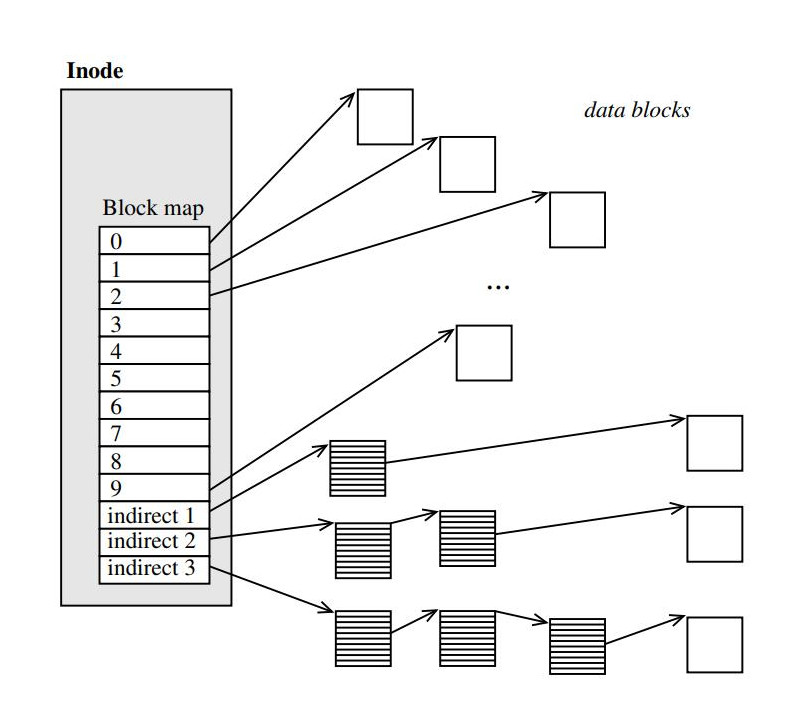
\includegraphics{6.2.2.jpg}}
    \caption{Z prezentace IOS: Souborové systémy, slide 23 -- odkazy v i-uzlech}
\end{figure}

\newpage

\subsubsection{Počty odkazů}
\begin{itemize}
    \item nepřímý odkaz 1. úrovně -- při 4 KiB clusteru je to $1024$ odkazů (1 odkaz = 4 B) = 1024 datových bloků,
    \item nepřímý odkaz 2. úrovně -- při 4 KiB clusteru je to $1024^2$ odkazů = stejný počet datových bloků,
    \item nepřímý odkaz 3. úrovně -- při 4 KiB clusteru je tam $1024^3$ odkazů = stejný počet datových bloků
\end{itemize}

\subsubsection{Limit maximální velikosti souboru}

Počtem přímých odkazů nepřímého odkazu 3. úrovně je dán maximální počet bloků, které je možné v tomto souborovém systému uložit. Teoretický limit velikosti souboru je tak:
\[
10 \cdot D + N \cdot D + N^2 \cdot D + N^3 \cdot D
\]
kde $D$ je velikost bloku v bajtech (běžně 4096~B), $M$ je velikost odkazů na blok v~bajtech (běžně 4~B), $N = D/M$, je počet odkazů v bloku.
 
Toto omezení velikosti je pouze jedním z omezení, která velikosti souboru omezují.
\textbf{Další omezení jsou daná:}
\begin{itemize}
    \item dalšími datovými strukturami a typy, které používá FS (např. datový typ délky souborů v bajtech v i-uzlu),
    \item strukturami VFS (veškerá práce s jakýmkoli FS musí projít přes VFS),
    \item rozhraním jádra,
    \item architekturou systému (32b -- velikost souboru bude 32b číslo + MSB je použit pro indikaci chyby [-1 bit pro data] -- soubory maximálně do 2~GiB, dnes běžná architektura 64b -- 64b velikosti)
\end{itemize}
 
Existuje \textbf{Large File System Support}, kde ve 32b systému se nahradí všechny údaje kde se pracuje s velikostí větším datovým typem -- podpora souborů \textit{větších než 2~GiB}.
 
\textbf{Linux:}

\textit{du [soubor]} vypíše zabrané místo v blocích vč. režie (metadat) \\[0.2em]
\textit{ls -l [soubor]} vypíše velikost souboru v bajtech (pouze užitečná data) \\[0.2em]
\textit{df} vypíše volné místo na discích \\[0.2em]
\textit{ls -i [soubor]} zpřístupní číslo i-uzlu souboru \\[0.2em]
\textit{is -e /dev/\ldots. n} -- výpis i-uzlu n na /dev/\ldots. \\[0.2em]
\textit{dumpe2fs} -- základní informace o souborovém systému ext2,3,4 \\[0.2em]
\textit{/dev/zero} je soubor typu zařízení generující proud nul \\[0.2em]
\textit{dd if=[source] of=[dest]} je nízkoúrovňové kopírování
 
\subsubsection{Výhody a nevýhody architektury FS}
Aneb proč byl navržen FS právě tak, jak byl. Architektura FS je totiž ovlivněna snahou o minimalizaci jejich režie s relativně pomalými disky (HDD, SDD), jedná se zejména o běžné operace se soubory, jako je průchod souborem (otevřu -- procházím od začátku do konce) či přesun (seek), zvětšování či zmenšování (vč. mazání) souborů.

\textbf{Je nutné vzít do úvahy, z jakých (mikro)operací se tyto operace skládají}. Jsou to operace:
\begin{itemize}
 \item vyhledávání adresy prvního nebo určitého bloku souboru,
 \item vyhledávání následujících bloků,
 \item přidání či odebrání bloků,
 \item alokace či dealokace volného souboru (informace o volných oblastech, minimalizace externí fragmentace)
\end{itemize}

FS a jeho následníci UFS, ext2, ext3 (ext4 už není jeho následník!) představují kompromis s ohledem převážně na malé soubory. (Tyto FS fungují skvěle pro malé soubory -- u větších souborů je nutné procházet či měnit větší objem metadat.)

Jistou optimalizací používanou i u klasických FS pro malé soubory je uložení dat přímo do i-uzlu (pokud se tam data vlezou).

\subsection*{Definice:}
\begin{description}
\item[symbolický odkaz] je soubor odkazující na jiný soubor (používá uložení dat přímo do i-uzlu)
\item[rychlé symlinky] mají data v i-uzlu
\item[pomalé symlinky] mají data mimo i-uzel
\end{description}

\subsection{Jiné způsoby organizace souborů}
\subsubsection{Kontinuální uložení}
\begin{itemize}
    \item neboli spojité uložení souboru na disku,
    \item na disku je jeden spojitý úsek dat reprezentující soubor,
    \item výhodami jsou rychlé vyhledání adresy určitého bloku nebo vyhledávání následujících bloků,
    \item nevýhody: soubory nebude možné jednoduše zvětšovat pokud budou příliš blízko u sebe (bude nutné jej přesunout na jiné volné a větší místo, pokud to půjde, či provést defragmentaci a poté zvětšit soubor)
    \item nepoužívá se příliš (kvůli své nevýhodě)
\end{itemize}

\subsubsection{Zřetězené seznamy alokačních bloků}
\begin{itemize}
    \item každý alokační blok obsahuje svá (užitečná) data a na konci obsahuje odkaz na následující alokační blok,
    \item výhodami jsou rychlý přístup na začátek či průchod daty,
    \item nevýhodou je přesun na náhodné místo v souboru -- nutnost přečíst celý soubor až po daný blok (1~GiB soubor, chci poslední blok -- musím přečíst celý),
    \item další nevýhodou je rozprostření metadat po celém disku -- při drobné chybě na disku přijdu o data (tedy i metadata, kde jsou odkazy na následující bloky) a dojde k velké ztrátě dat (všechna data za ztracenými daty jsou nepřístupná),
    \item není příliš vhodný, ale je jednoduchý, používá se v souborových systémech FAT
\end{itemize}

\subsubsection{FAT}
\begin{itemize}
    \item File Allocation Table,
    \item od zřetězených seznamů se liší tím, že seznamy popisující rozložení souborů na disku jsou uloženy v separátní oblasti na disku (tzv. FAT),
    \item data jsou ve FAT koncentrovaná -- rychleji se prohledávají, lze vytvořit více kopií FAT (prevence okamžité ztráty dat při chybě),
    \item stále vznikají problémy s rychlostí při náhodném přístupu (stále jde o zřetězený seznam),
    \item tabulka je pole, které obsahuje pro každý blok na disku 1 položku, každá položka obsahuje odkaz na další blok/položku,
    \item používá se i dodnes (a je to velmi rozšířené), protože je to jednoduché (např. vestavěné systémy)
\end{itemize}

\newpage

\subsubsection{B+ stromy}
\begin{itemize}
    \item jsou datovou strukturou převzatou z databázových systémů,
    \item mají dva typy uzlů -- vnitřní a listové,
    \item vnitřní uzly jsou kořen, jeho následníci (kromě listových) obsahují odkaz na následníka a vyhledávací klíč,
    \item listové uzly také obsahují odkazy a vyhledávací klíče, odkazy vedou na data na disku, poslední odkaz na posledním listu odkazuje na list na stejné úrovni (jsou tak propojeny lineárním seznamem),
    \item používají se za účelem popisu rozložení dat na disku (obsah souboru, poté vyhledávací klíč bude offset -- číslo logického bloku v rámci souboru) nebo se používají pro adresáře (klíče budou jména souborů) nebo pro popis celého obsahu disku (klíč je dvojice i-uzel a posuv souboru)
\end{itemize}
 
\textbf{Vyhledávání v B+ stromu:}
\begin{itemize}
    \item při hledání klíče $k$ se podívám, zda je klíč menší jak klíč $k_0$, pokud ano, půjdu níže, kde je $k_0$, pokud ne, zjistím, jestli je klíč mezi $k_0$ a $k_1$, pokud ano, jdu druhým směrem, opakuji po $k_n$,
    \item pokud jsem níž, opakuji to samé, co výš, dokud nedojdu k listovým uzlům,
    \item zde hledaný klíč najdu nebo zjistím že v této struktuře klíč není,
    \item poté mám odkaz na datový blok,
    \item v případě, že chci číst dál, jdu lineárně po sobě po následujících listových uzlech
\end{itemize}

\begin{figure}[htb]
    \centering
    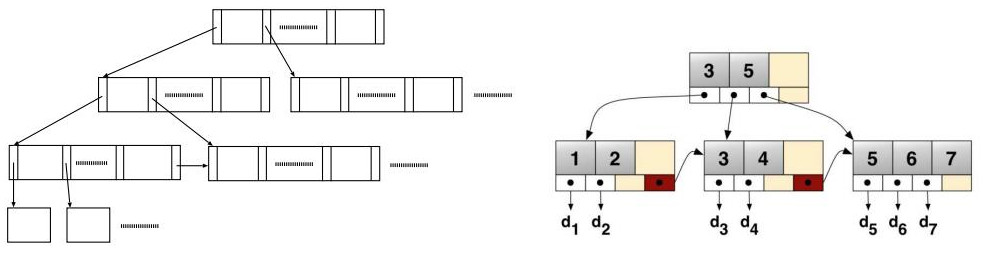
\includegraphics[width=\textwidth]{6.3.4.jpg}
    \caption{Z prezentace IOS: Souborové systémy, slide 27 -- B+ strom}
\end{figure}

\newpage

\textbf{Práce s B+ stromy:}
\begin{itemize}
    \item jsou zde limity, jak moc/málo mají být uzly zaplněné (strom se udržuje vyvážený) -- pro uzly s $m$ odkazy máme klíče $0, 1$, \ldots až $m - 2$ klíčů (odkazů je o 1 méně než klíčů + číslování od 0), 
    \item pokud je strom tvořen jediným kořenem -- nejméně může mít $1$ odkaz, maximálně $m - 1$ odkazů (poslední odkaz je použit jako ukončovač seznamu listů),
    \item pokud to není jediný kořen, tak má nějaké následníky, minimálně jich tak má $2$, maximálně $m$,
    \item vnitřní uzel tak má $\lceil\frac{m}{2}\rceil$ (zaokr. nahoru) až $m$ odkazů, list $\lceil\frac{m}{2}\rceil - 1$ (opět $\frac{m}{2}$ zaokr. nahoru) až $m - 1$ odkazů,
    \item vložení:
    \begin{itemize}
        \item nejprve projdeme stromem od kořene k listům,
        \item najdeme, kam chceme vložit,
        \item podíváme se, zda má list volný odkaz,
        \item pokud ano, použijeme ho, pokud ne, list se rozštěpí na 2 poloviny a podívám se o úroveň výš, zda je možné namísto 1 listu linkovat 2 listy,
        \item pokud ano, přidá se odkaz, pokud ne, nadřazený uzel se musí rozštěpit a postupovat o úroveň výš,
        \item \ldots štěpí se strom až případně se rozštěpí kořen a strom bude mít 2 kořeny
    \end{itemize}
    \item rušení:
    \begin{itemize}
        \item jde se opět od listové úrovně, tak, že se zruší odkaz v listu,
        \item zkontroluje se, zda je uzel zaplněný v rámci daných limitů,
        \item pokud ano, good, pokud ne, podívám se na sousední uzly a pokusím se provést přerozdělení tak, aby byly všechny uzly naplněný v rámci limitů,
        \item pokud se to nepodaří, tak dojde ke sloučení listů,
        \item posunu se o úroveň výš, zruším jeden odkaz, zkontrolují opět limity, zopakuji to samé,
        \item \ldots až se může stát, že se zruší i kořen
    \end{itemize}
\end{itemize}

B+ stromy a jeho varianty jsou používány pro popis diskového prostoru v souborových systémech jako XFS, JFS, ZFS, Btrfs, ReFS, \ldots, v omezené podobě tzv. stromu extentů v ext4, podobna struktura je i v NTFS.

\subsubsection{Extent}
\begin{itemize}
    \item používá se ke zrychlení práce s velkými soubory,
    \item umožňují zmenšit objem metadat (je možné říct, že některé alokační bloky jsou uloženy pospolu = vytváří extent), potom budu popisovat rozložení souborů po extentech (ne po alokačních blocích),
    \item přinese lépe vyvážené indexové struktury,
    \item rychlejší mazání,
    \item jsou použity snad ve všech systémech s B+ stromy,
    \item B+ strom se snadno kombinuje s extenty
    	\begin{itemize}\item neplatí pro klasický UNIXový strom, protože ve stromu jsou explicitně uložené vyhledávací klíče, ale UNIXový nemá v žádných strukturách (i-uzlech) uloženou velikost datových bloků (protože jsou všechny stejné a konstantní)\end{itemize}
\end{itemize}
 
Pokud používáme B+ stromy, tak rychlému spojitému průchodu pomáhá listová úroveň, pokud je prolinkování listů použito. Pro malé soubory může představovat B+ strom zbytečnou režii (data se buď uloží přímo v i-uzlu nebo nebo z něj máme přímé odkazy na extenty z i-uzlu, do max. 4 extentů).
 
\subsection*{Definice:}
\begin{description}
\item[extent] je jednotka vystavená na bloky, posloupnost proměnného počtu alokačních bloků (jdoucích za sebou logicky v souboru i fyzicky na disku).
\end{description}

\newpage

\subsection{ext4}
Používá pro popis rozložení dat na disku strom extentů. Pro „malé soubory“ (myšleno soubory, na které je možné se odkazovat až 4 extenty, pak tyto extenty budou odkazované přímo z i-uzlu; TLDR soubory s malým počtem extentů).
 
\subsection*{Definice:}
\begin{description}
\item[strom extentů] je v principu B+ strom degradovaný na maximálně 5 úrovní, bez používání vyvažování (např. přerozdělování uzlů při mazání) a zřetězení listu
\end{description}

\subsection{NTFS}
Základní datovou strukturou popisující disk je MFT -- Master File Table (má pro každý soubor alespoň 1 řádek, na 0. řádku popisuje samo sebe, 1. řádek případně kopie MFT, případně metadata, poté obsahy souborů).
 
\textbf{Obsah souboru může být reprezentován buď:}
\begin{itemize}
    \item pokud jde o krátký soubor, bude uložen v MFT v jeho řádku (včetně metadat),
    \item soubor je rozdělen na extenty (ty jsou odkazované přímo z řádků souboru v MFT, tak, že v řádce souboru jsou informace o počátečním VCN a LCN a počet clusterů, který daný extent obsahuje) -- vyhledává se v tom stejně jako v B+ stromu
    \item pokud je extentu potřeba více, než se vleze na jeden řádek, alokují se pomocné řádky (z hlavního řádku vedou odkazy na pomocné, z pomocných vedou odkazy na disk) -- procházení je opět ve stylu B+ stromu
\end{itemize}
 
\subsection*{Definice:}
\begin{description}
\item[VCN] -- virtual cluster number, logický blok souboru 
\item[LCN] -- logical cluster number, číslo fyzického bloku (souvisí s tím že je to na logickém disku)
\end{description}

\subsection{Organizace volného prostoru na disku}
V klasickém UNIXovém FS a řadě jeho následovníků (UFS, ext2, ext3), také v NTFS se používají bitové mapy, kde pro každý blok mám 1 bit. V bitové mapě je možné poté vyhledávat pomocí bitových mask -- zrychlí vyhledávání.
 
\textbf{Další možné způsoby organizace volného prostoru:}
\begin{itemize}
    \item použijí se alokační seznamy (zřetězení volných bloků na disku),
    \item zřetězení volných položek v tabulce (FAT),
    \item B+ strom (udržování informací o tom, kde je volné místo, adresace velikosti a/nebo offsetem)
    \item volný prostor může být také organizován po extentech
\end{itemize}

\newpage

\subsection{Deduplikace}
\begin{itemize}
    \item podporovaná ZFS, NTFS, Btrfs, XFS, \ldots (ext4 ne)
    \item snaží se odhalit opakované ukládání stejných dat na disk, uložit je pouze jednou a poté se na ně vícenásobně odkazovat,
    \item systémy s deduplikací se snaží taková data detekovat (sekvence bitů, bloků, extentů, \ldots)
    \item založeno na kryptografickém hashování (hledají se data se stejným popisem, určí se shoda),
    \item může být realizováno při zápisu nebo dodatečně (žádost uživatele),
    \item může uspořit diskový prostor (při virtualizaci, na mail serverech, repozitáře, \ldots), paměťový prostor i čas (zamezí se opakovanému čtení i zápisu),
    \item při menším objemu duplikace může naopak zvýšit spotřebu CPU času, spotřebu paměťového i diskového prostoru
\end{itemize}
 
\textbf{Rozdíl oproti copy-on-write:}
\begin{itemize}
    \item copy-on-write se může uchytit (klony, snímky) pouze tehdy, pokud duplikáty vzniknou činností samotného FS (např. vytvoření virtuálek),
    \item zatímco deduplikace aktivně vyhledává duplikáty (např. uživatel, co stahuje stejné reklamní letáky)
\end{itemize}

\subsection{Typy souborů v UNIXu}
\begin{itemize}
    \item - je obyčejný soubor,
    \item d adresář,
    \item b blokový speciální soubor,
    \item c znakový speciální soubor,
    \item l symbolický odkaz (symlink),
    \item p pojmenovaná roura,
    \item s socket
\end{itemize}

\subsection*{Definice:}
\begin{description}
\item[speciální soubor] je typ souboru reprezentující hardwarové zařízení (disk, paměť, \ldots), se kterým se komunikuje po blocích nebo znacích

\item[symbolický odkaz] je soubor obsahující jméno jiného souboru (odkazuje na něj)
\end{description}

\subsection{Adresář}
Adresář je kolekce jiných souboru na nejvyšší úrovni abstrakce. Soubor obsahuje množinu dvojic jméno a unikátní číselné označení.

\textbf{Jméno souboru:}
\begin{itemize}
\item dříve limit 14 znaků, dnes až 255 (na konci musí být \verb|'\0'|)
\item ve jméně nesmí být \verb|/| nebo '\verb|\0|'
\item platí, že každý adresář v POSIX systému vždy obsahuje minimálně 2 jména: \verb|.| (odkaz na sebe) a \verb|..| (odkaz na rodičovský adresář)
\end{itemize}

\textbf{Číslo souboru:}
\begin{itemize}
\item u klasického souboru UNIXu je to číslo i-uzlu,
\item v jiných případech to slouží jako klíč do dané vyhledávací struktury (B+ strom) \\
\end{itemize}

\textbf{Implementace adresářů:}
\begin{itemize}
\item používají se různé přístupy, liší se jednoduchostí implementace či rychlostí vyhledávání/vkládání,
\item seznam (obsah souboru bude tvořen seznamem),
\item B+ stromy (v NTFS, XFS, JFS, APFS nebo ext3/4 -- ty používají H-stromy: 1--2 úrovně, bez vyvažování a vyhledává se na základě zahashovaného jména)
\item hashovací tabulky v např. ZFS
\end{itemize}

Soubor v UNIXu může mít více jmen. Další jména se vytváří pomocí příkazu \verb|ln|.

\textbf{Linux:}
\tcmd{ln [existující jméno] [nové jméno]} vytvoří další jméno souboru

\subsection{Montování disku}
\textbf{Princip montování (připojování) disku:}
\begin{itemize}
\item v UNIXu není žádné označení disku (A:, C:, \ldots), ale máme jeden adresářový „strom“,
\item v systému je jeden kořenový logický disk,
\item další logické disky se připojují programem \tcmd{mount} do existujícího adresářového stromu (kořenový adresář zařízení se „slepí“ s adresářem v mém stromu)
\end{itemize}

Připojovací volby se mohou zadávat ručně (v terminálu) nebo se mohou předpřipravit do \tcmd{/etc/fstab}. Soubor \tcmd{/etc/mtab} obsahuje tabulku aktuálně připojených disků.

\textbf{Novější technologie umožňující automatické montování nově připojených zařízení:}

Na Linuxu běžně pracuje systém \emph{udev}, který
\begin{itemize}
\item rozpozná, že se připojilo nové zařízení,
\item vytvoří odpovídající soubor typu blokové zařízení (\tcmd{/dev/\ldots}),
\item informuje o tom zbytek systému pomocí sběrnice D-Bus,
\item aplikace typu správce souborů pak může provést automatické montování (a další akce),
\item přednost má vždy \tcmd{/etc/fstab},
\item identifikace se nemusí provádět jen zařízením (\tcmd{/dev/\ldots}), je možné si vygenerovat unikátní identifikátor a používat ten (\emph{UUID})
\end{itemize}

\textbf{Technologie Automounter:}
\begin{itemize}
\item subsystém jádra,
\item připojuje automaticky potřebné disky v situaci, kdy se pokusíme přistoupit na pozici adresářového stromu, kam by takovýto disk měl být připojeny (např. na \texttt{/mnt} má být připojena flashka, nemusí být mounted, uživatel dá \texttt{cd /mnt}, automounter to zjistí a připojí flashku sem),
\item má také nějaký čas, po kterém disk automaticky odpojí, pokud se ním nepracuje
\end{itemize}

\textbf{Union mount:}
\begin{itemize}
\item technologie umožňující sjednocující montování (v UNIXu dostupná pomocí souborového systému UnionFS),
\item umožňuje do jednoho přípojného bodu namontovat více disků,
\item obsah přípojného bodu je sjednocením obsahů disků,
\item v případě, že na více discích jsou soubory se stejnými jmény, vznikají kolize, ty se řeší např. předdefinováním priorit připojovaných FS a zpřístupní se soubor daného jména z logického disku, který má největší prioritu
\item UnionFS má copy-on-write sémantiku, což umožňuje emulaci přepisování nepřepisovatelných médií (v jedné větvi nepřepisovatelné CD, například s Linuxovou distribucí, současně se do stejného bodu připojí běžný disk s vyšší prioritou -- na začátku bude disk prázdný, budou vidět všechny soubory z CD, jakmile se pokusím přepsat něco, UnionFS vytvoří kopii na přepisovatelný disk)
\end{itemize}

\textbf{Linux:}
\tcmd{mount [co-pripojit] [kam-pripojit]} připojí logický disk

\newpage
\section{}
\textbf{Sedmá přednáška:} Pokračování správy souborů, symbolické odkazy.

\subsection{Symbolické odkazy}
\begin{itemize}
    \item symbolické odkazy jsou samostatné soubory odkazující na existující soubor,
    \item systém při otevření automaticky otevře cílový soubor -- vícenásobné zpracování cesty (cesta k symlinku a cesta uvnitř něj),
    \item soubor se smaže, pokud jeho počet jmen klesne na 0,
    \item symlink může odkazovat na neexistující soubor (při otevření dojde k chybě),
    \item může odkazovat i na jiný logický disk,
    \item ze symlinků lze vytvořit cyklus (jeden odkazuje na druhý a druhý na první) -- v systému je předdefinovaný maximální počet na sebe odkazujících symlinků (při překročení dojde k chybě),
    \item symlinky lze využít např. při upgradu systému.
\end{itemize}
 
\textbf{Rozdíl rychlých a pomalých symlinků:}
\begin{itemize}
    \item obsahem symlinku je jméno cílového souboru,
    \item pokud jméno souboru není příliš dlouhé (vleze se do i-uzlu), potom se uloží do i-uzlu = rychlý symlink (stačí otevřít jen i-uzel),
    \item pokud se jméno nevleze do i-uzlu, alokují se normálně alokační bloky na disku = pomalý symlink
\end{itemize}
 
\textbf{Linux:}
\tcmd{ln -s [existující soubor] [symbolický odkaz]} vytvoří symbolický odkaz
 
\subsection{Blokové a znakové speciální soubory} \label{blok-char-hw}
Soubory reprezentující rozhraní souborového systému k fyzickým (opravdový HW) či virtuálním zařízením (terminály, \ldots). Souborový systém vytváří souborové rozhraní, tím umožňuje tyto soubory při určitých operacích identifikovat (jméno souborů, např. \tcmd{/dev/sdX}), s celým zařízením lze také pracovat jako se souborem.
 
Typicky zařízení sídlí v adresáři \tcmd{/dev}.
 
\textbf{Běžné typy zařízení:}
\begin{itemize}
    \item /dev/hda -- (dříve) označení pro první \emph{fyzický} disk na prvním ATA/PATA rozhraní
    \item /dev/hda1 -- (dříve) první \emph{logický} disk na hda
    \item /dev/sda -- první fyzický disk SCSI, navíc i disky SATA/PATA (jádro nad těmito disky emuluje SCSI)
    \item /dev/mem -- obsah paměti (RAM)
    \item /dev/zero -- nekonečný zdroj nul (bajtů 0)
    \item /dev/null -- soubor typu černá díra -- cokoli se do něj zapíše, zahodí se (přesměrování výstupů programů tak, aby nás neotravoval), při čtení se tváří jako prázdný soubor
    \item /dev/random, /dev/urandom -- generátor (pseudo)náhodných čísel
    \item /dev/tty -- terminál
    \item /dev/lp0 -- tiskárny
    \item /dev/mouse -- myš
    \item /dev/dsp -- zvuková karta
    \item /dev/loop -- zařízení typu smyčka, umožňuje připojit \textbf{soubor jako disk} (obraz souborového systému) k adresáři, jako by se jednalo o nový fyzický disk
\end{itemize}
 
Tato označení závisí na použitém systému (Linux, distribuce, \ldots). Výhoda zavedení speciálních souborů je, že umožňují identifikovat zařízení, se kterými chci pracovat.

\newpage

\subsection{Přístupová práva}
V UNIXu jsou typicky rozlišena na práva pro \emph{vlastníka}, \emph{skupinu vlastníků} a \emph{ostatní}. Existuje rozšíření \emph{ACL} (Access Control List).
 
\textbf{Uživatelé:}
\begin{itemize}
    \item jsou definováni administrátorem systému (root) v \tcmd{/etc/passwd},
    \item mají definovaná svá UID -- uživatelská čísla (root UID = 0),
    \item každý soubor má svého vlastníka,
    \item \tcmd{chown} -- změna vlastníka souboru (pouze root)
\end{itemize}
 
\textbf{Skupiny:}
\begin{itemize}
    \item definuje administrátor systému v \tcmd{/etc/group},
    \item mají svá GID -- číslo identifikující skupinu uživatelů,
    \item v každé skupině je uvedeno, kdo do té skupiny patří,
    \item každý uživatel může být členem více skupin,
    \item jedna z nich je aktuální (používá se při vytváření souboru)
\end{itemize}
 
\textbf{Linux:}

\tcmd{groups} -- výpis skupin uživatele \\[0.2em]
\tcmd{chgrp} -- změna skupiny souboru \\[0.2em]
\tcmd{newgrp} -- nový shell s jiným aktuálním GID

\subsection{Typy přístupových práv}
\textbf{Obyčejné soubory:} r, w, x -- právo číst, zapisovat a spustit soubor jako program.
 
\textbf{Adresáře:}
\begin{itemize}
    \item r -- právo číst obsah adresáře,
    \item w -- právo zapisovat (vytvářet a rušit soubory),
    \item x -- právo přistupovat k souborům v adresáři (možnost provést např. \tcmd{cd [adresář]}, \ldots)
\end{itemize}
 
\textbf{Typický výstup přístupových práv je:}
\begin{itemize}
    \item ve formátu: [1:typ souboru] [3:práva vlastníka] [3:práva skupiny] [3:práva ostatních]
    \item např.: -rwx---r-- (číselné vyjádření v osmičkové soustavě: 0704) je obyčejný soubor, vlastník má všechna práva, skupina žádná a ostatní mají práva na čtení
\end{itemize}
 
Změna přístupových práv se děje pomocí \tcmd{chmod}. (Pro nespustitelné soubory je běžný chmod 0644).
 
\textbf{Linux:}
\tcmd{chmod [1:pro koho][nová práva] [soubor/y]} změna přístupových práv

\subsection{Sticky bit}
Příznak, který pokud bude přiřazen nějakému adresáři, tak se vytvoří adresář, ve kterém i přes právo čtení a zápisu souborů mohou uživatele rušit pouze ty soubory, které sami vytvořili. Typickým příkladem je adresář \tcmd{/tmp}. (TLDR: uživatel může mazat, ale pouze to, co vlastní).

\newpage
\subsection{(S|E)UID, (S|E)GID} \label{seuid}
\textbf{S procesy jsou spojeny různé identifikátory, např.:}
\begin{itemize}
    \item UID -- reálná identifikace uživatele (číslo uživatele, který daný proces spustil)
    \item EUID -- efektivní identifikátor používaný pro kontrolu přístupových práv (většinou stejné jako UID)
    \item GID -- reálná identifikace skupiny (kdo spustil proces)
    \item EGID -- efektivní GID (stejné chování jako u EUID)
\end{itemize}
 
Vlastník programu může propůjčit svá práva komukoliv, kdo spustí program s nastaveným SUID bitem. (Běžně se to používá v případech, kdy administrátor propůjčuje svá práva uživatelům, např. \tcmd{passwd} nebo \tcmd{ping}).
 
Při použití SUID bitu bude UID = uživatele, který proces spustil a EUID = identifikace vlastníka (= který práva půjčil). Pokud budou práva propůjčená (použito SUID), místo x se vypíše s, pokud tam x není, vypíše se S.

\subsection{Typická struktura adresářů v UNIXu}
\textbf{FHS -- Filesystem Hierarchy Standard (Linux), (část hierarchie):}
\begin{itemize}
    \item /bin -- programy pro všechny uživatele (spustitelné, mohou být zapotřebí při bootování, musí být dostupné lokálně)
    \item /boot -- soubory pro zavaděč systému (obrazy jádra, počáteční FS)
    \item /dev -- rozhraní zařízení (speciální soubory)
    \item /etc -- konfigurační soubory pro systém i aplikace
    \item /home -- domovské adresáře uživatelů
    \item /lib -- sdílené knihovny a moduly jádra
    \item /media -- přípojný bod pro přenosná zařízení
    \item /mnt -- přípojný bod pro (dočasné) FS
    \item /proc -- informace o procesech a jádru
    \item /root -- domovský adresář superuživatele
    \item /run -- dočasné informace o běžícím systému (démoni)
    \item /sbin -- programy pro superuživatele (nutné pro bootování, ne vše je spustitelné superuživatelem)
    \item /sys -- informace o jádru, zařízeních, modulech, \ldots
    \item /tmp -- dočasné pracovní soubory (obsah se maže při restartu)
    \item /usr -- obsahuje dále adresáře a soubory, které nejsou nutné při zavádění systému, struktura je zde podobná jako u \tcmd{/}
    \begin{itemize}
        \item bin, sbin, lib,
        \item include (hlavičkové soubory),
        \item share (soubory je možné sdílet nezávislé na architektuře),
        \item local (kořen další hierarchie určená pro lokální nestandardní instalace programů),
        \item src (zdrojové texty jádra)
    \end{itemize}
    \item /var -- soubory měnící se za běhu systému
    \begin{itemize}
        \item log (záznamy o činnosti systému), 
        \item spool (pomocné soubory pro tisk),
        \item mail (poštovní přihrádky uživatelů)
    \end{itemize}
\end{itemize}

\newpage

\textbf{Nové téma: Datové struktury a algoritmy pro vstup a výstup}

\subsection{Použití vyrovnávacích pamětí}
Cílem použití cache (vyrovnávacích pamětí) je minimalizace počtu pomalých operací s periferiemi (disky). Hierarchie:
kolekce, sbírka dílčích vyrovnávacích pamětí (s velikostí jednoho alokačního bloku, či násobku), nazývá se buffer-pool, může mít pevnou velikost, ale obvykle se mění.

\subsection{Operace se soubory}
\subsubsection{Čtení}
\textbf{První čtení alokačního bloku:}
\begin{itemize}
    \item zjistí se, zda je blok v paměti,
    \item pokud ne, naalokuje se nový blok, může se využít již nějaký systémem předalokovaný a nevyužitý,
    \item načtou se data z disku, přesunou se do vyrovnávací paměti,
    \item vyrovnávací paměť je v prostoru jádra (běžné procesy zde nemají přístup),
    \item vykousne se z načtených dat ta část, o kterou má uživatel/proces zájem,
    \item nakopíruje se to do adresového prostoru uživatelského prostoru
\end{itemize}
 
\textbf{Při dalším čtení:}
\begin{itemize}
    \item nejprve se opět vyhledá, zda je blok v paměti,
    \item pokud ano, nebude se číst z disku, pouze se z alokačního bloku vykousne část, o kterou má uživatel/proces zájem,
    \item tato část se uživateli předá
\end{itemize}
 
\subsubsection{Zápis}
 
\textbf{Postup při zápisu:}
\begin{itemize}
    \item nejprve se zjistí, zda je blok v paměti,
    \item pokud ne, přidělí se vyrovnávací paměť,
    \item načtou se data z disku do vyrovnávací paměti,
    \item jádro převezme od procesu, který chce zapisovat, data, která chce zapsat,
    \item přepíše jimi danou část alokačního bloku, dirty bit se změní (0 na 1),
    \item operace končí (neprovede se zápis na disk),
    \item časem se provede zpožděný zápis na disk a vynuluje se dirty bit \\
\end{itemize}
 
Systém sám od sebe s periodou přepisuje obsah z caches na disky, lze si to vynutit pomocí sync či fsync.
 
Pokud je známo, že se přepíše celý alokační blok (nebo se jedná o nový blok), buffer se vynuluje a nenačítají se data z disku do cache.

\subsection*{Definice:}
\begin{description}
\item[dirty bit] je indikátor toho, jestli jsou data cache sladěna s obsahem na disku (0 -- data v cache jsou shodná s těmi na disku, 1 -- data cache != data disk -- nuluje se zpožděným zápisem)
\end{description}

\subsubsection{Otevření souboru pro čtení}
Pokud soubor ještě \textbf{nebyl otevřen}:
\begin{itemize}
    \item systém musí vyhodnotit cestu a najít číslo i-uzlu (resp. číslo datové struktury poskytující informace o daném souboru -- přístupová práva, kde jsou uložena data),
    \begin{itemize}
        \item při tom se postupně načítají i-uzly všech adresářů vedoucí na soubor,
        \item poté se načte i-uzel souborů,
        \item systém používá \emph{d-entry cache} (speciální vyrovnávací paměť použitá pro překlad odpovídajících jmen souborů na i-uzel) 
        \item dále alokuje položku v tabulce \textbf{V-uzlu},
        \item z disku se načte i-uzel,
        \item vloží se do nově alokované položky = vzniká rozšířená paměťová kopie i-uzlu,
        \item budou tam i informace navíc (jako je počet odkazů na danou položku -- s daným i-uzlem může pracovat více procesů).
    \end{itemize}
    \item v tabulce popisovačů vytvoříme novou položku,
    \begin{itemize}
        \item tato tabulka je uložena v záznamu o procesu (tabulka procesu v jádře) nebo v uživatelské oblasti,
        \item použije se nejnižší volná položka zde,
        \item naplní se odkazem na položku v tabulce otevřených souborů,
    \end{itemize}
    \item pokud se otevření vydaří, vrátí se číslo popisovače, pokud ne, tak vrací -1.
\end{itemize}
 
Tolik tabulek se používá pro zamezení duplikaci údajů. Během otevírání se provádí kontrola přístupových práv. Soubor je možné otevřít v režimu pro čtení, zápis, nebo čtení i zápis.
 
Další otevření souboru (\textbf{již jednou otevřeného}):
\begin{itemize}
    \item opět se vyhodnotí cesta k souboru a získá se číslo i-uzlu,
    \item systém se podívá do tabulky V-uzlů,
    \item zjistí, že i-uzel už tam je,
    \item nebude se znovu i-uzel načítat z disku, pouze se zvýší čítač použití i-uzlu,
    \item tabulka V-uzlu musí být vyhledávací (typicky vyhledávací struktury jako hash tabulka, strom, \ldots),
    \item naalokuje se nová položka v tabulce otevření (náplní se režimem otevření, pozicí, odkazem na sdílený V-uzel),
    \item naalokuje se nově položka ve file descriptoru ukazující na nové otevření (a ta se vrátí)
\end{itemize}
 
\textbf{Je možné přidávat i další identifikátory, např.:}
\begin{itemize}
    \item příznak, že má být soubor vytvořen, pokud neexistuje,
    \item pokud existuje, má být zkrácen na 0,
    \item otevřít v režimu přidávání (kdekoli je aktuálně ukazovátko v souboru, tak v případě zápisu se automaticky posune na konec a tam se přidá),
    \item synchronní zápis (operace zápisu skončí až tehdy, když se data zapíšou opravdu na disk)
\end{itemize}
 
\textbf{Při chybě:}
\begin{itemize}
    \item \tcmd{open()} vrací -1,
    \item nastaví se chybový kód, který blíže popisuje, co se stalo (do knihovní proměnné \tcmd{errno}),
    \item existují standardní chybové kódy,
    \item lze použít standardní knihovní funkci \tcmd{perror()}
\end{itemize}
 
\subsection*{Definice:}
\begin{description}
\item[V-uzly] je v podstatě tabulkou i-uzlů souborového systému VFS

\item[tabulka popisovačů] je pole s řádky číslovanými od 0 (0: stdin, 1: stdout, 2: stderr)

\item[tabulka procesů v jádře] je část adresového prostoru, ve kterém má jádro uložené pomocné informace k procesům a má sem přístup pouze jádro
\end{description} 
 
\textbf{Linux:} \\
\tcmd{fd = open([jméno souboru], [režim])} otevře soubor

\subsubsection{Čtení a zápis z/do souboru}
\textbf{Čtení:}
\begin{itemize}
    \item zkontroluje se platnost popisovače (otevření popisovače, soubor pro čtení),
    \item pokud se jedná o první přístup, naalokuje se cache, načtou se data do cache a z cache se příslušná data použijí,
    \item pokud už jsou data v cache, načtou se odtud,
    \item předání se děje z cache (RAM, jádro) do pole (RAM, část adresového prostoru procesu),
    \item funkce vrací počet opravdu přečtených bajtů nebo -1 při chybě (+ nastaví errno).
\end{itemize}

\textbf{Zápis:}
\begin{itemize}
    \item funguje podobně jako \tcmd{read()},
    \item před vlastním zápisem kontroluje dostupnost diskového prostoru a tento prostor alokuje (rezervuje),
    \item vrací počet opravdu zapsaných bajtů nebo -1
\end{itemize}
 
\textbf{Linux:}

\tcmd{read}([popisovač], [adresa paměti, kam se má zapsat], [kolik bajtů se má načíst]): přečte soubor \\[0.2em]
\tcmd{write}([popisovač], [adresa paměti, ze které se načtou data], [kolik bajtů se zapíše]): zápis do souboru
 
\subsubsection{Přímý přístup k souboru}
Náhodné přesouvání v souboru. \textbf{Postup:}
\begin{itemize}
    \item zkontroluje, zda je popisovač platný (je soubor otevřen?)
    \item nastaví pozici
    \begin{itemize}
        \item SEEK\_SET -- např. 200 -- posunu se od 200 bajtů od začátku,
        \item SEEK\_CUR -- od aktuální pozice,
        \item SEEK\_END -- od konce souboru,
    \end{itemize}
    \item nelze se posunou před začátek souboru,
    \item je ale možné se posunout za konec souboru (a zapsat),
    \item vrací se výsledná pozice od začátku souboru nebo -1
\end{itemize}
 
Posunem za konec souboru a následným zápisem vznikají tzv. \emph{řídké soubory} (sparse files):
\begin{itemize}
    \item umožňuje na disku o nějaké kapacitě vytvořit soubor, který má zdánlivě větší velikost než samotný disk,
    \item bloky do kterých se nezapisovalo nejsou alokovány a nezabírají diskový prostor (při čtení se považují za 0),
    \item také může vzniknout mazáním uprostřed souboru (hole punching)
\end{itemize}
 
\begin{figure} [ht]
    \centering
    \scalebox{2}{
\includegraphics{7.9.5.jpg}} \\
    \caption{Z prezentace IOS: Správa souborů -- řídké soubory} 
\end{figure}
 
\textbf{Linux:}
\tcmd{lseek}([popisovač souboru], [offset], [oproti čemu se chci posouvat]): přímý přístup k souboru
 
\newpage

\subsubsection{Zavření souboru}
\begin{itemize}
    \item zkontroluje se platnost file descriptoru (je vůbec otevřený?),
    \item uvolní se daná položka v tabulce popisovačů,
    \item systém se podívá na odkazovanou položku v tabulce otevřených souborů,
    \item sníží se počítadlo o 1,
    \item pokud bude počítadlo != 0, uzavírání skončí,
    \item pokud bude počítadlo == 0, pokračuje se do 
    \item příslušné položky tabulky V-uzlu, sníží se zde počítadlo o 1,
    \item pokud bude zde počítadlo != 0, uzavření skončí,
    \item pokud bude zde == 0, soubor se definitivně uzavře,
    \item z tabulky V-uzlu se uvolní z paměti i-uzel (se změněnými údaji -- čas zápisu, přístupů, modifikace i-uzlu, \ldots),
    \item naplánuje se blok, ve kterém je i-uzel uložen,
    \item časem se i-uzel zapíše na disk,
    \item funkce vrací 0 nebo -1 při chybě
\end{itemize}
 
Pokud se proces ukončí, automaticky se zavřou všechny jeho deskriptory. Uzavření souboru nezpůsobí uložení obsahu jeho vyrovnávací paměti na disk.
 
\textbf{Linux:}
\tcmd{close}([popisovač souboru]) zavře soubor

\subsubsection{Duplikace deskriptoru souboru}
\begin{itemize}
    \item zkontroluje se platnost deskriptoru (je soubor otevřen?),
    \item zkopíruje obsah původního popisovače do nového (odkaz ve fd tabulce se zkopíruje do další položky v této tabulce -- oboje ukazují na stejnou položku tabulky otevřených souborů + inkrementuje se počitadlo), 
    \item automaticky se nový deskriptor uzavře (pokud je otevřen),
    \item vrací index nově vytvořené položky nebo -1,
    \item typické použití je u přesměrování (stdin/stdout)
\end{itemize}
 
\textbf{Linux:}
\tcmd{dup}([popisovač]) duplikace deskriptoru (duplikuje existující popisovač do nejvyššího volného nového) \\[0.2em]
\tcmd{dup2}([popisovač], [nový popisovač]) duplikace deskriptoru (do kterého popisovače se duplikuje)

\subsubsection{Rušení souboru}
\begin{itemize}
    \item vyhodnotí se cesta, zkontroluje se platnost jména souboru, přístupová práva (zápis),
    \item odstraní se pevný odkaz (=hard link) mezi jménem souboru a i-uzlem,
    \item zmenší se počet jmen v i-uzlu,
    \item pokud je počet jmen == 0 a i-uzel nikdo nepoužívá, i-uzel může být uvolněn a mohou být uvolněny všechny bloky souborů,
    \item dokud má soubor alespoň 1 jméno nebo nemá žádné jméno ale je alespoň jednou otevřen, nelze soubor z disku opravdu smazat,
    \item funkce vrací 0 nebo -1 při chybě
\end{itemize}
 
Je možné provést unlink na otevřený soubor (smaže se až po jeho uzavření) a pracovat s ním dále -- využití při instalacích nových verzích programů, které aktuálně běží.
 
\textbf{Linux:}
\tcmd{unlink}([jméno souboru, příp. cesta]) ruší soubor \\[0.2em]
\tcmd{shred} -- bezpečné mazání

\subsubsection{Další operace se soubory}

\textbf{Linux:}

\tcmd{creat, open} -- vytvoření souboru \\[0.2em]
\tcmd{rename} -- přejmenování souboru \\[0.2em]
\tcmd{truncate, ftruncate} -- zkrácení souboru \\[0.2em]
\tcmd{fcntl, lock} -- zamykání záznamů \\[0.2em]
\tcmd{chmod, chown} -- změna atributů \\[0.2em]
\tcmd{utime}- -- umožňuje změnit časy práce se soubory (neumožňuje změnit čas modifikace i-uzlu) \\[0.2em]
\tcmd{stat} -- získání atributů (velikost, práva, \ldots) \\[0.2em]
\tcmd{sync, fsync} -- vynucení si zápisu vyrovnávacích pamětí na disk

\subsubsection{Adresářové soubory}
Obsahuje dvojice číslo i-uzlu a jména souborů. Adresáře nelze zapisovat či číst po bajtech.

\textbf{Linux:}

\tcmd{mkdir} -- tvoří se adresáře (vytvoří položky \lpath{.} a \lpath{\ldots}) \\[0.2em]
\tcmd{opendir} -- otevře adresář \\[0.2em]
\tcmd{readdir} -- čte adresář \\[0.2em]
\tcmd{closedir} -- zavře adresář \\[0.2em]
\tcmd{creat, link, unlink} -- modifikace se provádí nepřímo vytvářením a modifikacemi souborů

\subsubsection{Blokové a znakové speciální soubory}
Představují rozhraní k blokovým, či znakovým zařízením (\lpath{/dev/\ldots}, viz \ref{blok-char-hw}).
\begin{itemize}
\item lze je vytvořit pomocí \tcmd{mknod},
\item typicky tyto soubory vytváří jádro či démoni (udev, devd -- při připojení zařízení se vytvoří automaticky příslušný soubor)
\end{itemize}

Při použití běžných souborových operací jádro mapuje operace na odpovídající podprogramy, které ty operace implementují pro daný typ zařízení s využitím \textbf{tabulek}:
\begin{itemize}
\item znakových zařízení,
\item blokových zařízení
\end{itemize}

Tyto tabulky obsahují ukazatele na funkce implementující příslušné operace v ovladačích daných zařízení.

Speciální soubory na disku zabírají \textbf{pouze i-uzel}, kromě běžných údajů mají v i-uzlu typ souboru a 2 dvadaje:
\begin{itemize}
\item hlavní číslo,
\begin{itemize}
\item major number,
\item udává typ zařízení
\item odkazuje do tabulky zařízení (hlavní číslo = $n$-tý řádek tabulky),
\end{itemize}
\item vedlejší číslo 
\begin{itemize}
\item minor number, 
\item udává instanci zařízení
\item používá se jako parametr při volání určité operace -- parametr funkce ovladače (číslo = které zařízení se má přesně použít)
\end{itemize}
\item typ souboru určuje tabulku (blok., znak.)
\end{itemize}

\textbf{Linux:}

\tcmd{mknod} vytvoří speciální soubory \\[0.2em]
\textit{\textbf{ovladač}} je sada podprogramů pro řízení určitého typu zařízení (viz \ref{ovladace} nebo \ref{ovladac})

\subsection{Terminály}
Terminály jsou fyzická či logická zařízení umožňující (primárně) textový vstup a výstup systémů (po řádcích), editaci vstupního řádku či použití speciálních znaků (Ctrl+C vyvolává SIGINT, Ctrl-D značí konec vstupu, \ldots).
 
\textbf{Rozhraní:}
\begin{itemize}
    \item /dev/tty -- pro každý proces, který má řídicí terminál, odkazuje na jeho řídicí terminál
    \item /dev/ttyS1 -- fyzické terminály na sériové lince,
    \item /dev/tty1 -- virtuální terminály (konzole),
    \item pseudoterminály (/dev/ptmx -- master, /dev/pts/1, \ldots) tvořený dvojicí master/slave, po každém otevřením se vytvoří nový slave -- emuluje komunikaci přes sériovou linku (umožňuje pro propojení určitých částí, např. SSH -- propojení klienta se vzdáleným klientem) \\
\end{itemize}
 
\textbf{Různe režimy zpracování znaků} (řádkové disciplíny, line discipline):
\begin{itemize}
    \item raw -- neprovádí se zpracování znaků,
    \item cooked -- zpracování všech řídicích znaků,
    \item cbreak -- provádí zpracování malého počtu znaků (Ctrl+c, mazání, \ldots)
\end{itemize}
 
Nastavení režimu zpracování znaků je možné pomocí \tcmd{stty}. Dále je možné nastavit \textbf{režim terminálu}:
\begin{itemize}
    \item příkazy \tcmd{tset}, \tcmd{tput}, \tcmd{reset}, \ldots
    \item proměnná TERM, ve které je uložen aktuální typ terminálu,
    \item typy terminálů (příkazy \tcmd{terminfo}, \tcmd{termcap})
\end{itemize}
 
Tyto příkazy komunikují s terminálem pomocí \textit{escape sekvencí}. Knihovna \texttt{curses} je standardní knihovna pro řízení terminálů či tvorbu aplikací s terminálovým uživatelským rozhraním.
 
\subsection*{Definice:}
\begin{description}
\item[escape sekvence] jsou sekvence znaků escape, příkaz [parametry], escape, příkaz, \ldots
\end{description}

\newpage

\subsection{Roury}
Roury jsou prostředkem meziprocesové komunikace. Rozlišujeme:
 
\textbf{Nepojmenované roury}
\begin{itemize}
    \item nemají adresářovou položku, tedy neexistují v souborovém systému,
    \item lze s nimi pracovat pouze tak, že se vytvoří pomocí volání \tcmd{pipe} (vrátí čtecí a zápisový deskriptor), jakmile dojde k uzavření, práce s rourou končí,
    \item mohou s ní pracovat běžně pouze příbuzné procesy,
    \item je dostupná pomocí popisovačů z tabulky popisovači (při klonu procesu se naklonuje popisovací tabulka -- proces bude ukazovat na stejné místo v tabulce otevřených souborů),
    \item jediná výjimka, jak je možné odkaz na nepojmenovanou rouru předat, je přes UNIXové sockety (kromě klonování procesu),
    \item vytváří se v kolonách (např. paralelně běžící procesy p1 | p2 | p3 -- na přesměrování se používají nepojmenované roury)
\end{itemize}
 
\textbf{Pojmenované roury}
\begin{itemize}
    \item vytvářejí se pomocí \tcmd{mkfifo},
    \item existují v souborovém systému,
    \item mohou se zavřít, otevřít, apod.
\end{itemize}
 
Roury slouží jako mechanismus meziprocesové komunikace. Implementované jsou jako kruhový buffer s omezenou kapacitou. Procesy komunikující přes rouru jsou synchronizovány.
 
\subsection*{Definice:}
\begin{description}
\item[příbuzné procesy] -- pokud jeden proces otevře rouru a začne se \textit{klonovat} (viz \ref{fork}), všechny tyto procesy mohou s rourou pracovat

\item[konzumenti] -- procesy, které čtou

\item[producenti] -- procesy, které zapisují
\end{description}

\newpage

\section{}
\textbf{Osmá přednáška:} Dokončení souborových systémů: roury, sockety, VFS. Procesy.

\subsection{Sockety}
Umožňují jak síťovou (klient-server, TCP, UDP), tak lokální (souborový systém) komunikaci.
 
Pro vytvoření socketu se používá volání \tcmd{socket}:
\begin{itemize}
    \item následně se čeká na připojení (\tcmd{bind} -- propojit socket s TCP/UDP portem či souborem, \tcmd{listen} -- začínám čekat, \tcmd{accept} -- příjem příchozího spojení),
    \item klient se připojí pomocí \tcmd{connect},
    \item příjem a vysílání zpráv (\tcmd{recv}/\tcmd{send} či \tcmd{read}/\tcmd{write} -- volání vrací popisovače otevřených souborů),
    \item uzavření (\tcmd{close})
\end{itemize}
 
Sokety podporují blokující i neblokující I/O. Při práci s více sockety je možné je obsluhovat více procesy či vlákny (příkaz \tcmd{select}) -- typy souborů, u kterých může nastat potřeba čekat na možnost provedení určité operace. Sokety taky mají výhodu, že je možné vytvořit aplikace, které mohou běžet distribuovaně v síti.
 
\subsection*{Definice:}
\begin{description}
\item[blokující režim] -- pokud chci načítat data ze socketu, budu pozastaven, dokud se nějaká data neobjeví

\item[select] umožňuje testovat, zda na popisovači (či na množině popisovačů) je dostupná nějaká operace 

\item[pasivní čekání] -- nespotřebovává se CPU čas, energie, \ldots
\end{description}
 
\subsection{VFS} \label{VFS-new}
Virtual File System. Definice viz \ref{VFS-old}. Komunikace s různými FS se přenáší z uživatele na autora FS, který pokud chce, aby daný FS byl využitelný, musí ho provázat s VFS (propojení VFS a uživatele řeší vývojáři).
 
Typická datová struktura VFS jsou \textbf{V-uzly} = rozšířené paměťové kopie i-uzlu, které kromě dat i-uzlu obsahují další data:
\begin{itemize}
    \item jako počet odkazů na V-uzel z tabulky otevřených souborů, 
    \item ukazatele na funkce implementující operace nad i-uzlem (v patřičném FS).
\end{itemize}
 
\subsection{NFS} \label{NFS-more}
Network File System. Zpřístupňuje soubory uložené na vzdálených systémech.
 
Jedná se o \textbf{systém klient-server}:
\begin{itemize}
    \item klient požádá např. o čtení ze souboru,
    \item všechny operace prochází přes VFS,
    \item požadavek se z VFS předá na NFS klienta,
    \item NFS klient předá požadavek na NFS server,
    \item NFS server pracuje s lokálním FS již na vzdáleném PC,
    \item ten pracuje také s VFS (ale na serveru), prostřednictvím něj získá data z lokálního FS,
    \item data poté putují přes síť zpět k uživateli.
\end{itemize}
 
Umožňuje \textbf{kaskádování} -- je možné si lokálně do jednoho adresářového stromu připojit vzdálený strom (a do něj připojit další vzdálený souborový systém). \textbf{Autentizujeme se nejčastěji přes UID, GID} (musí existovat důvěra mezi správcem lokálního a vzdáleného systému), může ale používat i jiné mechanismy (kryptografie, \ldots).
 
NFS verze 3:
\begin{itemize}
    \item starší, bezstavová verze -- nepoužívá operace otevírání, uzavírání souborů, každá operace si musí nést veškeré informace o souboru,
    \item na straně klienta nemá cache (složitá implementace), na straně serveru cache,
    \item nemá podporu zamykání (operace pro zamknutí záznamu souboru jsou prázdné).
\end{itemize}
 
NFS verze 4:
\begin{itemize}
    \item stavová,
    \item cache na straně klienta,
    \item podpora zamykání.
\end{itemize}

\subsection{Spooling}
Simulatenous perpiheral operation on-line (simultánní online provádění periferních operací). Jedná se o \textbf{provádění online operací bez čekání periferní operace (výstup) na periferiích, které nemusí online prokládání dat od různých procesů či uživatelů podporovat}. (Příklad: síťová tiskárna -- spousta uživatelů, každý chce, aby tisk se provedl okamžitě.)
 
Výstup se provede do vyrovnávací paměti spool (soubor), systém si vede frontu čekajících úloh, operaci, do fronty se zařadí odkaz na vytvořený soubor, úloha se dokončí po uvolnění periferie.
 
\textbf{Linux:}
\lpath{/var/spool} obsahuje soubory spool
 
\newpage
\textbf{Nové téma:} Správa procesů.
 
Správa procesů (process management) zahrnuje: \label{procesy-detailed}
\begin{itemize}
    \item přepínání kontextu (\emph{dispatcher}, vždy v režimu jádra),
    \item plánovač (nemusí být v jádře),
    \item správu paměti,
    \item podporu meziprocesové komunikace (signály, roury, sockety, synchronizace -. semafory, mutexy, \ldots)
\end{itemize}
 
\subsection*{Definice:}
\begin{description}
\item[přepínáním kontextu] rozumíme fyzické odebírání procesoru jednomu procesu a přidělování jinému procesu (také viz \ref{prepinani-kontextu-jadro})

\item[plánovač] rozhoduje, který proces či procesy poběží a případně jak dlouho
\end{description}

\subsection{Proces}
Definice viz \ref{procesy}. Proces je běžící program, tedy aktivní entita, abstrakce aktivity probíhající v systému. Program je naopak pasivní entita (definice viz \ref{procesy}).
 
\textbf{Proces je v OS definován:}
\begin{itemize}
    \item unikátním identifikátorem (PID -- process identifier),
    \item stavem plánování,
    \item řídicím programem,
    \item obsahem registru (běžných -- EAX, EBX, EIP, \ldots),
    \item zásobníkem (aktivační záznamy -- informace o rozpracovaných funkcích),
    \item daty (statická ne/inicializovaná data, hromady, individuálně alokovaná paměť),
    \item tím, jaké další vazby a zdroje OS využívá (jaké soubory má aktuálně otevřené, signály, obslužné funkce signálů, PPID, UID, GID, semafory, sdílená paměť, sdílené knihovny, \ldots)
\end{itemize}
 
\subsection{Stavy plánování a jejich změny}
Nejzákladnější plánovací diagram (většiny různých OS) -- \textbf{stavy procesu}.
 
\textbf{Stavy plánování procesů (obecně):}
\begin{itemize}
    \item new -- proces je inicializován (vytváří se struktury, co jej popisují, data, proces případně čeká ve vstupní frontě dlouhodobého plánovače, \ldots)
    \item ready -- proces čeká na krátkodobý plánovač na přidělení procesoru, dispatcher provede přepnutí, přepne se do running
    \item running -- proces může být přerušen (preemptivni plánování -- opět stav ready), může požádat o službu jádro (I/O operace, sync) -- stav waiting,
    \item waiting -- proces čeká na dokončení operace (služba jádra), poté půjde do stavu ready,
    \item terminated -- proces skončí (proces se v systému nějakou dobu vyskytuje ve stavu ukončený)
\end{itemize}

% obrazek 5/38, sprava procesu
\begin{figure} [ht]
    \centering
    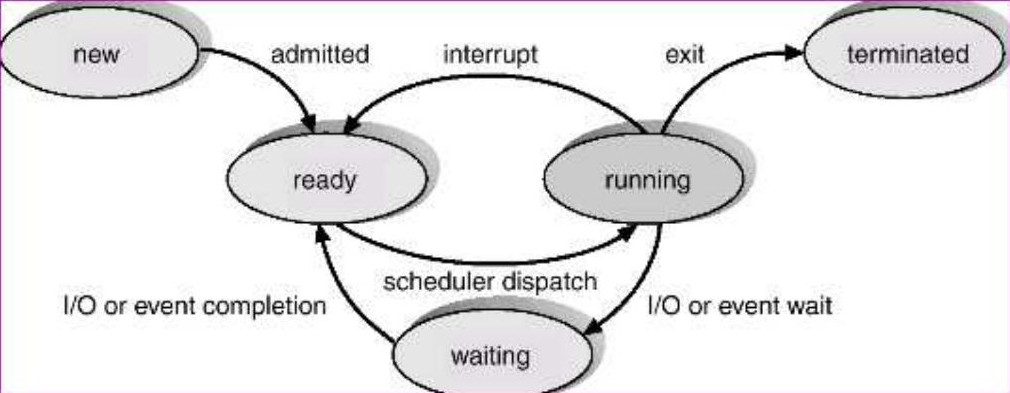
\includegraphics[width=\textwidth]{8.6_1.jpg}
    \caption{Z prezentace IOS: Správa procesu -- stavový diagram obecného plánování procesu}
\end{figure}

\newpage

\textbf{Stavy plánování procesů v UNIXu:}
\begin{itemize}
    \item init -- vytvořený, neinicializovaný,
    \item runnable -- připraven běžet,
    \item running -- proces běží (přidělen procesor), v případě preempce (proces se vzdá CPU) jde do runnable,
    \item sleeping -- proces požádá o I/O či sync akci (čeká na dokonce operace), po realizaci bude runnable
    \item suspended -- pomocí signálu SIGSTOP může být proces zmrazen a čeká čeká na rozmrazení (signál SIGCONT),
    \item zombified -- ukončení procesů a přechod do stavu zombie (mátoha), proces skončil, odebrány všechny zdroje, pouze o něm zůstává záznam v tabulce procesů (zde je jeho návratový kód, dokud si ho někdo nepřevezme)
\end{itemize}
 
% obrázek 6/38, správa procesů
\begin{figure} [ht]
    \centering
    \scalebox{2}{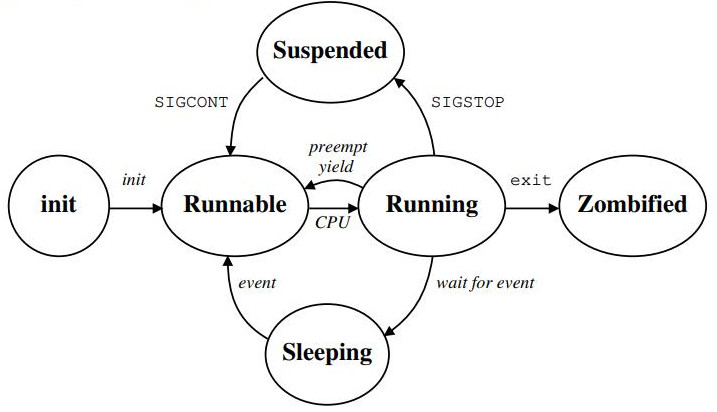
\includegraphics{8.6_2.jpg}}
    \caption{U prezentace IOS: Správa procesů -- stavový diagram plánování procesů v UNIXu}
\end{figure}
 
OS s procesem pracuje tak, že je reprezentován pomocí struktury PCB (process control block), někdy také task control block či task struct. \label{pcb}
 
\textbf{PCB zahrnuje (přímo nebo formou odkazů):}
\begin{itemize}
    \item identifikátory spojené s procesem,
    \item stav plánování,
    \item obsah registru (v okamžiku, kdy je pozastaven),
    \item plánovací informace (priorita, ukazatele na plánovací fronty, \ldots),
    \item informace spojené se správou paměti (tabulky stránek při použití stránkované paměti),
    \item informace spojené s účtováním (sumarizuje informace o běhu procesu -- spotřeba CPU, \ldots),
    \item informace o využití I/O zdrojů (otevřené soubory, tabulka popisovačů, \ldots)
\end{itemize}
 
PCB může být buď jedna struktura nebo může být rozděleno na několik částí.

\subsection{Části procesu v paměti v UNIXu}
První součást paměti využité procesem je \textbf{uživatelský adresový prostor} (user address space) -- je přístupný procesu (může z této části paměti číst a psát do ní), obsahuje:
\begin{itemize}
    \item kód (který je řízen, code area/text segment),
    \item data (ne/inicializovaná, hromada, alokovaná paměť),
    \item zásobník,
    \item soukromá data sdílených knihoven, sdílené knihovny či sdílená paměť
\end{itemize}
 
Další část informací o procesech bývá v některých případech (ne vždy) umístěna v \textbf{uživatelské oblasti} (např. Linux tento koncept nepoužívá, vše má v tabulce procesů):
\begin{itemize}
    \item informace jsou uloženy pro každý proces v části uživatelského adresového prostoru, která \textit{není procesům přístupná},
    \item je to přístupné jádru,
    \item u každého procesu si v této části ukládá informace o procesu,
    \item je tam:
    \begin{itemize}
    \item část PCB, která je používána zejména za běhu procesu,
    \item PID, UID, EID, GID, EGID, PPID (identifikátor rodiče),
    \item obsah registrů,
    \item deskriptory souborů (informace o tom, který deskriptor je použit jako stdin, stdout),
    \item obslužné funkce signálů (funkce, které se budou volat pro obsluhu signálů),
    \item účtování,
    \item pracovní, kořenový adresář
    \end{itemize}
\end{itemize}
 
\textbf{Další záznamy jsou v tabulce procesů:}
\begin{itemize}
    \item uloženo trvale v jádru,
    \item informace o procesu, které jsou důležité, i když proces neběží:
    \item PID, PPID, UID, EID, \ldots,
    \item stav plánování,
    \item událost, na kterou proces čeká,
    \item plánovací informace (pro plánovač -- při rozhodování, který proces dál poběží či ne -- podle priority, spotřeba času, viz \ref{planovani}),
    \item čekající signály (signály, které mohou přijít, i když proces neběží),
    \item odkaz na tabulky dat reprezentující rozložení procesů, dat, kódů, zásobníků, \ldots
\end{itemize}
 
\newpage
 
Poté jsou ještě záznamy v \textbf{tabulce paměťových regionů:}
\begin{itemize}
    \item jak je rozdělen uživatelský adresový prostor na regiony (= souvislý kus paměti použitý pro kód, zásobník, \ldots),
    \item velikost těchto regionů,
    \item globální tabulka regionů (odkaz z této na lokální tabulky regionů),
    \item regiony bývají členěny na stránky (tabulky stránek)
\end{itemize}
 
\subsection*{Definice:}
\begin{description}
\item[logický adresový prostor] je rozsah všech logických adres, které se mapují do fyzické paměti
\item[zásobník jádra] je separátní zásobník, který je někdy používán pro ukládání rozpracovaných funkcí jádra v okamžiku, kdy jádro provádí službu pro daný proces
\end{description}

\subsection{Kontext procesu}
Kontext je jiné označení pro \textbf{stav procesu}. Rozlišujeme:
\begin{itemize}
    \item uživatelský kontext -- část stavu procesu popisující část paměti dostupnou procesu samotnému (kód, zásobník, data),
    \item registrový kontext,
    \item systémový kontext -- část stavu procesu nedostupná samotnému procesu (uživatelská oblast, položky tabulky procesů, paměťové regiony, \ldots)
\end{itemize}

\subsection{Systémová volání nad procesy UNIXu}
= standardní POSIXová volání:
\begin{itemize}
    \item fork, exec, exit, wait, waitpid,
    \item kill, signal -- synchronizace,
    \item getpid, getppid -- získávání identifikátorů, \ldots
\end{itemize}
 
\textbf{Identifikátory spojené s procesy v UNIXu:}
\begin{itemize}
    \item identifikace procesu PID (vlastní identifikátor procesu),
    \item identifikace předka PPID (proces, který daný proces vytvořil, rodič),
    \item uživatel (a skupina), který proces spustil -- UID, GID,
    \item efektivní uživatel či skupina -- EUID, EGID (viz \ref{seuid}),
    \item uložené EUID a EGID -- procesům umožňují dočasně se zbavit vysokých práv, která získal (proces se dobrovolně vzdá vyšších práv --- uloží se a poběží s běžnými právy -- v okamžiku provádění kritických operací si práva zase navýší -- ochrana před chybami v programech),
    \item v Linuxu FSUID, FSGID (filesystem UID/GID -- oddělená zvýšená privilegia pro práci s FS),
    \item PGID, SID (process group identifier, session identifier -- skupina procesů či sezení, do kterých proces patří)
\end{itemize}
 
\subsection*{Definice:}
\begin{description}
\item[sezení] je skupina skupin procesů vytvářející se typicky při práci s terminály
\end{description}

\subsection{Vytváření procesu} \label{fork}
Procesy v UNIXu vznikají \textbf{voláním služby \tcmd{fork}}. Fork je volání, které se \textbf{zavolá jednou}, pokud nedojde k chybě, \textbf{skončí dvakrát}. Na základě volání fork vzniká \textbf{vztah rodič-potomek} (parent-child) a hierarchie procesů. Výsledkem forku je totiž \textbf{duplikace procesu}. Vzniká takřka identická kopie potomka, který dědí:

\begin{itemize}
    \item řídicí kód, data, zásobník, sdílenou paměť, otevřené soubory, obsluhu signálů, většinu synchronizačních prostředků, \ldots
    \item pro efektivitu používá pro práci s pamětí copy-on-write
    \item kopie se liší v návratovém kódu \tcmd{fork}, identifikátorech, údajích spojených s plánováním a účtováním, nedědí se čekající signály, souborové zámky a některé další zdroje či nastavení
\end{itemize}
 
\textbf{Návratové kódy fórků:}
\begin{itemize}
    \item $0$: fork se zdařil, \verb|if (pid == 0) { kód potomka }|
    \item $-1$: fork se nezdařil, \verb|if (pid == -1) { kód rodiče }|
    \item cokoli jiného (PID potomka): \verb|else { kód rodiče }|
\end{itemize}
 
\subsection{Hierarchie procesu v UNIXu}
Prvním procesem, který vzniká a vytváří jej jádro, je \textbf{proces \tcmd{init} s PID=1} (novější a aktuálně často používaná implementace: \tcmd{systemd}). Tento proces je \textbf{předkem všech ostatních uživatelských procesů}. \textbf{PPID initu je 0}.
 
Existují také procesy jádra (kernel threads/processes), jejich předkem \tcmd{init} \textbf{není}:
\begin{itemize}
    \item jejich kód je součástí jádra,
    \item vyskytuje se i proces s PID=0, vzniká úplně jako první, podílí se na inicializaci jádra, následně se mění na swapper (pokud je na systému použit) nebo na čekací smyčku nebo je to používáno jako procesová obálka pro vlákna jádra (na Linuxu se tento proces nevypisuje)
\end{itemize}
 
\tcmd{init} se podílí na \textbf{inicializaci systému}, poté \textbf{přebírá návratové kódy procesů, které osiřely dřív, než skončily} (tedy rodič skončí dřív než potomek) -- teoreticky by byl zombie procesem do nekonečna, proto \tcmd{init} přebírá jeho návratový kód a umožní mu odchod ze systému.
 
\subsection*{Definice:}
\begin{description}
\item[swapper] je proces, který v případě akutního nedostatku paměti některé procesy pozastaví a zcela uloží na disk (veškeré části paměti zabírané procesem)

\item[kthread] je (na Linuxu) „init procesem“ pro procesy jádra, má PID=2 
\end{description}

\textbf{Linux:}
\tcmd{pstree} výpis stromu procesů

\subsection{Změna programu -- \tcmd{exec}}
Umožňuje v rámci existujícího procesu „vyměnit jeho vnitřnosti“ -- \textbf{zahodit existující kód a nahradit ho kódem jiným}. \tcmd{exec} je funkce, která se \textbf{zavolá jednou a neskončí vůbec} (je v nějakém kódu, ten kód přestane běžet) pokud nedojde k chybě.
 
Pokud v procesu zavolám \tcmd{exec}:
\begin{itemize}
    \item dědí řadu rysů svého předka,
    \item zůstává mu řada zdrojů a vazeb s OS (identifikátory, otevřené soubory, \ldots),
    \item zanikají vazby a zdroje vázané na původní kód (obslužné funkce signálů, sdílená paměť, paměťově mapované soubory, semafory).
\end{itemize}
 
Skupina funkcí exec:
\begin{itemize}
    \item \tcmd{execve} (základní volání), \tcmd{execl}, \tcmd{execlp}, \tcmd{execle}, \tcmd{execv}, \ldots
\end{itemize}
 
Ve Windows se procesy vytváří voláním \tcmd{CreateProcess(\ldots)}, které zahrnuje funkčnost \tcmd{fork} i \tcmd{exec}.

\subsection{Čekání na potomka -- \tcmd{wait, waitpid}}
Slouží k tomu, aby mohl \textbf{rodič čekat na dokončení činnosti svých potomků}.

Volání \tcmd{wait}:
\begin{itemize}
 \item čeká na ukončení \emph{jednoho z potomků},
 \item vrací číslo potomka, který skončil (případně $-1$ pokud přijde signál, který čekání přeruší, nebo pokud čekáme na potomka a žádného nemáme),
 \item může to být operace blokující, pokud žádný z potomků ještě neskončil, 
 \item pokud některý potomek skončil dřív před voláním \tcmd{wait}, volání okamžitě skončí a vrátí se návratový kód potomka.
\end{itemize}

Volání \tcmd{waitpid}:
\begin{itemize}
 \item umožňuje čekání na ukončení určitého potomka určité skupiny dle PID,
 \item umožňuje čekání i na pozastavení či probuzení (SIGSTOP, SIGCON).
\end{itemize}

\subsection{Start systému}
\begin{itemize}
 \item (nejprve) dostane se ke slovu firmware PC (UEFI/BIOS),
 \item načtení a spuštění zavaděče OS (někdy se zavaděčů používá několik, např. BIOS využíval základní kód MBR -- série zavaděčů),
 \item načtou se inicializační funkce jádra a samotné jádro, spuštění inicializačních funkcí,
 \item inicializační funkce jádra vytvoří proces 0, další procesy jádra a proces \tcmd{init},
 \item proces \tcmd{init} pokračuje v inicializaci systémy, spouští démony a procesy,
 \item v určitém okamžiku se z něj spustí procesy umožňující práci s X Window System a přihlášení v GUI (GDM, SDDM, LightDDM),
 \item na konzolích se spustí \tcmd{getty} (\textit{Ctrl+Alt+F1, F2, \ldots}) -- umožní uživateli zadat přihlašovací jméno, změní se na \tcmd{login}, načte od uživatele heslo, poté se změní na shell, ze kterého se spouští další procesy, po ukončení se opět spouští \tcmd{getty},
 \item proces \tcmd{init} i po inicializaci nadále běží, přebírá návratové kódy procesů, jejich rodič skončil dřív než příslušný proces, také řeší reinicializaci systému (na přání uživatele či výpadek napájení)
\end{itemize}

\subsection*{Definice:}
\begin{description}
\item[firmware] je program uložený v nevolatilních pamětech, provádějící kontrolu HW a případnou inicializaci HW
\end{description}

\newpage

\subsection{Úrovně běhu}
Systém úrovní běhu byl zaveden již v UNIX System V. Rozlišují se úrovně běhu 0--6: (některé měly předpřipravený standardní význam, některé si definoval administrátor)
\begin{itemize}
    \item 0 = halt -- zastavení systému,
    \item 1/s/S = single user mode -- jednouživatelský režim, používá správce systému pro administrativní úlohy,
    \item 6 = reboot -- automatické restartování systému,
    \item ostatní runlevely (2--5) definovány na různých systémech různě,
    \item je možné změnit úrovně běhu (režimy) pomocí \tcmd{tellinit [N]}.
\end{itemize}
 
Konfigurace úrovní běhu:
\begin{itemize}
    \item v adresáři \lpath{/etc/rcX.d} (X=úroveň běhu) jsou skripty spouštěné při vstupu do dané úrovně,
    \item nejprve se volají skripty začínající písmenem $K$ v pořadí daném číslem za tím $K$ (volají se s argumentem \tcmd{stop}),
    \item poté se volají skripty začínající $S$ (volají se s argumentem \tcmd{start}),
    \item start, stop -- definuje se co se má spustit či jak se co má zastavit,
    \item v adresáři \lpath{/etc/init.d} vytvoříme skript, který požadovanou službu bude umět spouštět, na patřičné místo K a S odkazů se vytvoří symlink na požadovaný skript,
    \item skripty v \lpath{init.d} typicky přijímají parametry \tcmd{start}, \tcmd{stop}, \tcmd{reload}, \tcmd{restart}
    \item tyto skripty se nemusí volat pouze při změně úrovně běhu, ale je možné je volat i ručně -- z \lpath{/etc/init.d}
    \item v souboru \lpath{/etc/inittab} je horní, hlavní úroveň systému, kde se popisuje např. implicitní úroveň běhu či jaké úrovně běhu jsou podporované
\end{itemize}

Existují různé nové implementace procesu \tcmd{init} -- dnes nejběžnější je \tcmd{\textbf{systemd}}:
\begin{itemize}
    \item základní úrovně běhu jsou nahrazeny jednotkami (\emph{units}), které mají různé typy (targets, services, \ldots),
    \item spouští inicializační jednotky paralelně na základě jejich závislostí (výhodou je, že inicializaci systému je možné provádět paralelně, zatímco \tcmd{init} postupuje sekvenčně),
    \item emulují se úrovně běhu (zpětná kompatibilita),
    \item užitečné jsou adresáře \lpath{/lib/systemd} či \lpath{/usr/lib/systemd}
\end{itemize}
 
\subsection{Plánování procesů} \label{planovani}
Procesy plánuje \emph{plánovač}.
 
Rozlišujeme 2 základní \textbf{plánovací algoritmy} (definice viz \ref{ne-preemtive}):
\begin{itemize}
    \item nepreemptivní plánování (typicky I/O operace, konec -- volání \tcmd{exit}, proces se sám musí vzdát CPU -- \tcmd{yield}),
    \item preemptivní plánování (typicky přerušení od časovače, může jít i o jiné, třeba od disku)
\end{itemize}

Rozlišujeme \textbf{3 „typy“ plánování}:
\begin{itemize}
    \item dlouhodobé plánování -- které úlohy budou připuštěny do systému,
    \item střednědobé plánování -- procesy paměť mají, nebo nemají -- jedná se o systém swapování,
    \item krátkodobé plánování -- procesy mají paměť -- přepínání mezi úlohami
\end{itemize}
 
\textbf{Systém swapování} (= střednědobé plánování):
\begin{itemize}
    \item v případě nedostatku paměti některé procesy pozastaví, odebere jim veškerou paměť a uloží je na disk,
    \item tyto procesy jsou vyřazeny z plánování (nemají paměť -- nemohou běžet),
    \item při žádosti o spuštění úlohy úloha pak nebude spuštěna ihned, ale systém čeká na uvolnění systémových zdrojů (služba čeká ve frontě) -- poté už se jedná o dlouhodobé plánování (rozhoduje se o tom, které úlohy budou vůbec připuštěny do systému)
\end{itemize}
 
\subsection*{Definice:}
\begin{description}
\item[plánovač] rozhoduje, který proces či procesy poběží (a případně jak dlouho)
\item[systémy s nepreemptivním plánováním] = systémy s kooperovaným plánováním (procesy musí aktivně spolupracovat, kooperovat)
\end{description}

\subsection{Přepnutí kontextu (procesu)}
Přepnutí kontextu na příkladu -- dispečer na základě rozhodnutí plánovače přepíná mezi procesem A a B:
\begin{itemize}
    \item bude muset uchovat stav registrů (některých, ale včetně řídicích registrů) procesu A do PCB (nebo task struct v Linuxu; viz \ref{pcb}),
    \item dojde k úpravě některých řídicích struktur v jádře (úprava plánovacích struktur, účtovacích struktur, \ldots),
    \item obnova uložených hodnot registrů procesu B,
    \item dojde k předání řízení procesu na adresu, kde bylo dříve přerušeno provádění procesu B,
    \item tato akce se musí provádět v režimu jádra
\end{itemize}
 
Neukládá se a neobnovuje celý stav procesu (při pozastavení procesu není nutné na disk ukládat obsah paměti, ukládají se pouze registry).
 
Přepnutí může trvat \textbf{řádově stovky až tisíce instrukcí/cyklů} -- jádra umožňují měnit interval, v jakém přicházejí přerušení z časovače -- je třeba si dát pozor, aby ten interval nebyl příliš krátký, protože začne poté převažovat režie systému nad užitečným během (neustálé ukládání a obnovování obsahů registrů).

\newpage

\section{}
\textbf{Devátá přednáška:} Dokončení správy procesů.

\subsection{Klasické plánovací algoritmy}
\subsubsection{FCFS}
\begin{itemize}
    \item \emph{first come, first served},
    \item plánovací algoritmus založený na jednoduché FIFO frontě,
    \item proces, který nově vznikne nebo je uvolněn z čekání na nějaké operaci (I/O, sync, \ldots), případně proces, který se vzdá CPU, se zařadí na konec fronty,
    \item procesy, které poběží, se vybírají ze začátku fronty,
    \item jedná se o nepreemptivní algoritmus (k přepnutí kontextu dojde, pouze pokud se běžící proces vzdá CPU či zavolá službu jádra)
\end{itemize}
 
\subsubsection{Round-robin}
\begin{itemize}
    \item preemptivní obdoba FCFS,
    \item pracuje podobně jako FCFS,
    \item každý proces má přiděleno nějaké časové kvantum,
    \item jakmile je mu přidělen CPU, proces běží a poběží nanejvýš po dobu časového kvanta,
    \item po vypršení času je procesu odebrán CPU a je zařazen na konec fronty,
    \item CPU se přidělí procesu ze začátku fronty
\end{itemize}
 
\subsubsection{SJF}
\begin{itemize}
    \item \emph{shortest job first},
    \item nejprve se provede nejkratší úloha,
    \item algoritmus přiděluje CPU tomu procesu, který aktuálně deklaruje nejkratší dobu pro svůj další běh na CPU, po který nebude žádat o žádné I/O operace (tzv. CPU burst),
    \item běh úloh se dělí na výpočetní práce (CPU burst) a poté na periody, kdy se komunikuje s periferiemi (disky, sítě, \ldots),
    \item nepreemptivní algoritmus (nepřerušuje proces před dokončením jeho aktuální výpočetní fáze),
    \item statisticky minimalizuje průměrnou dobu čekání a zvyšuje propustnost systému,
    \item je nutné dopředu znát dobu běhu procesu na CPU v jejích jednotlivých výpočetních fázích, respektive musí existovat možnost tyto doby rozumně odhadnout (na základě předchozího chování těchto úloh),
    \item dává smysl pro opakovaně prováděné úlohy, 
    \item používá se zejména v dávkových (specializovaných) systémech,
    \item nevýhodou algoritmu je náchylnost ke \textbf{stárnutí} při čekání na nějaký zdroj (CPU, zámek, \ldots)
    \begin{itemize}
        \item pokud nějaký proces deklaruje délku CPU burst a v systému budou neustále kratší procesy s touto délkou, tyto procesy ho budou neustále předbíhat (nikdy se tak k CPU nedostane)    
    \end{itemize}
\end{itemize}

\subsection*{Definice:}
\begin{description}
\item[stárnutí] (hladovění, starvation) je situace, kdy některý proces, který žádá o zdroj, na daný zdroj čeká bez záruky, že jej někdy získá.
\end{description}
 
\subsubsection{SRT}
\begin{itemize}
    \item \emph{shortest remaining time},
    \item preemptivní obdoba SJF
\end{itemize}

\subsubsection{Víceúrovňové plánování}
\begin{itemize}
    \item procesy rozdělené do různých skupin (typicky dle priority, ale ne nutně -- např. dle typu procesu),
    \item každá skupina procesu může používat jiný dílčí plánovací algoritmus (FSFS, round-robin, SJF, \ldots) s různými parametry,
    \item kromě toho máme další („hlavní“) algoritmus, který rozhoduje, která skupina procesů dostane CPU čas -- často jednoduše na základě priorit skupin,
    \item poté je další plánovací algoritmus, který plánuje mezi skupinami
\end{itemize}
 
\subsubsection{Víceúrovňové plánování se zpětnou vazbou}
\begin{itemize}
    \item skupiny procesů jsou rozděleny dle priorit,
    \item proces, který se stane nově připraveným běžet (nově vznikne, je uvolněn z čekání, \ldots) je zařazen do skupiny procesů s nejvyšší prioritou,
    \item v této skupině běží a postupně klesá do nižších priorit,
    \item až spadne do nejnižší úrovně (plánován round-robin),
    \item používají se varianty, kdy proces má přednastavenou statickou prioritu a zařadí se do plánovací úrovně této priority, a poté má i dynamickou prioritu, která se může zvyšovat i snižovat, typicky se priority mění tak, že pokud nějaký proces spotřebovává mnoho CPU času, priorita se sníží; pokud proces čeká na mnoho I/O operací, priorita se zvýší,
    \item cílem je zajistit rychlou reakci interaktivních procesů (=komunikujících s uživatelem),
\end{itemize}

\subsection{Plánovač v Linuxu (od verze 2.6.23)}
Používá se \textbf{víceúrovňové prioritní plánování se 100 základními statickými prioritními úrovněmi}:
\begin{itemize}
    \item priority 1-99 jsou vyhrazeny pro procesy reálného času (algoritmy FCFS s preempcí na základě priorit nebo round-robin),
    \item priorita 0 jsou běžné procesy plánované \emph{CFS} plánovačem (viz níže),
    \item v rámci úrovně 0 se používají \emph{podúrovně} v rozmezí -20 až 19, nejvyšší podúroveň je -20 (je možné běžně uživatelsky nastavovat příkazy \tcmd{nice} a \tcmd{renice}),
    \item v rámci úrovně 0 se rozlišují 3 typů procesů: běžné, dávkové a idle,
    \item základní prioritní úroveň (RT proces v 1-99, běžný proces) a typ plánování (round-robin, FCFS, \ldots) je možné nastavit pomocí služby \tcmd{sched\_setscheduler},
    \item později přidáno plánování pro sporadické periodické úlohy -- založeno na strategii \emph{earliest deadline first} (převzato z realtimových OS) \\
\end{itemize}
 
\subsection*{Definice:}
\begin{description}
\item[FCFS s preempcí na základě priorit] --  pokud během běhu procesu doběhne I/O operace či \tcmd{sync} operace, která způsobí proveditelnost procesů s vyšší prioritou, dojde k přepnutí kontextu  (nedochází k přepnutí kontextu na základě časových kvant s procesy s stejnou prioritou)

\item[dávkové procesy] mají mírnou penalizaci z hlediska priorit, mají ale delší kvantum

\item[idle procesy] mají nízkou prioritu, předpokládá se, že se dostanou ke slovu až v okamžik, když v systému nic užitečnějšího není

\item[sporadické periodické úlohy] jsou úlohy, které běží, mají periodické výpočetní fáze (očekávaná fáze -- známe dobu jak dlouho trvají + máme časový limit, dokdy se mají výpočty provést), které se provádějí čas od času
\end{description}

\subsection{Completely Fair Scheduler}
CFS plánovač:
\begin{itemize}
    \item snaží se explicitně každému procesu poskytnout odpovídající procento strojového času s ohledem na jeho priority (4 procesy, stejná priorita $\Rightarrow$ všechny 25 \% CPU času),
    \item u každého procesu si vede údaje o tom, kolik virtuálního CPU času už ten proces na CPU strávil,
    \item vede si údaj o minimálním stráveném CPU čase (dává nově připraveným procesům),
    \item procesy udržuje ve vyhledávací struktuře (red-black tree) podle využitého CPU času,
    \item při rozhodování, který proces poběží, ze struktury vezme ten, který aktuálně strávil nejméně času na CPU,
    \item proces nechá běžet po časové kvantum, které spočítá na základě priorit,
    \item \textbf{virtuální procesorový čas}: situace: 2 procesy běžící celý den (každý půl dne), přijde nový proces, fyzicky na CPU běžel 0 s (nejvyšší priorita, běžel by půl dne a ty 2 by byly off), proto virtuální CPU čas -- nový proces dostane čas menší než minimální strávený čas všemi procesy (ne 0),
    \item algoritmus má podporu pro skupinová plánování, umí rozdělovat čas spravedlivě pro skupiny procesů (spouštěné z různých terminálů, od různých uživatelů, \ldots)
\end{itemize}

\subsection{Plánování ve Windows NT a novějších}
\begin{itemize}
    \item Používá se víceúrovňové prioritní plánování se zpětnou vazbou na základě interaktivity:
    \item 32 prioritních úrovní: 
    \begin{itemize}
        \item 0: nulování volných stránek paměti (aby se nedostaly informace od jednoho uživatele/procesu k jinému)
        \item 1--15: běžné procesy
        \item 16--31: procesy reálného času
    \end{itemize}
    \item základní priorita procesu je dána kombinací plánovací třídy a plánovací úrovně (v rámci třídy),
    \item priorita se dynamicky snižuje či zvyšuje:
    \item zvýší se priorita procesů spojených s oknem, které je v popředí,
    \item zvýší se priorita procesů spojených s oknem, do kterého přichází vstupní zprávy (myš, časovač, klávesnice, \ldots),
    \item zvýší se priorita procesů uvolněných z čekání (I/O operace),
    \item zvýšená priorita se po každém vyčerpání kvanta sníží o jednu úroveň (až do dosažení základní priority)
\end{itemize}
 
\subsection{Inverze priorit}
Jedná se o \textbf{problém, nežádoucí stav}, který je nutné řešit!
\begin{itemize}
    \item jedná se o situaci, kdy v OS máme různé prioritní procesy, málo prioritní proces si naalokuje si nějaký zdroj, zamkne si přístup k nějakému sdílenému zdroji (soubor, adresa v paměti, síťový port, \ldots),
    \item procesy s vyšší prioritou tyto procesy předbíhají, 
    \item proces s nižší prioritou se čas od času dostane ke slovu, provede pár instrukcí, musí čekat,
    \item (má naalokovaný zdroj, chce s ním něco provést, to ale trvá dlouho, protože ho pořád někdo předbíhá),
    \item může nastat, že některý z prioritních procesů potřebuje právě ten zdroj, který si zamkl tento nízkoprioritní proces,
    \item proces s vyšší prioritou bude muset čekat -- \emph{virtuálně} se zvýší (rapidně) priorita nízkoprioritíiho procesu (= je to vedlejší efekt, reálně má prioritu pořád stejnou!),
    \item v systému je možné mít procesy se střední prioritou, které tento zdroj nepotřebují, ty budou předbíhat dále nízkoprioritní proces,
    \item proces s vysokou prioritou musí čekat, zatímco procesy se střední a nižší prioritou mají najednou „pomyslně vyšší prioritu“,
    \item tento jev může a nemusí vadit -- může způsobit sníženou odezvu systému, nicméně můžou se zablokovat i některé kritické procesy reálného času (ovládání hardware, \ldots)
\end{itemize}

\textbf{Možnosti řešení inverze priorit:}
\begin{itemize}
    \item prioritní strop (priority ceiling -- procesy v kritické sekci získávají nejvyšší prioritu,
    \item priority inheritance -- procesy v kritické sekci, které blokují procesy s vyšší prioritou, po dobu běhu v kritické sekci dědí prioritu čekajícího procesu (s nejvyšší prioritou),
    \item na jednoprocesorových systémech se používá technika, kdy se po dobu běhu v kritické sekci zakáže přerušení
\end{itemize}

Další komplikace během plánování:
\begin{itemize}
 \item víceprocesorové systémy -- nutné vyvažovat výkon (aby na jednom jádru CPU neběžely 4 procesy a na zbytku 0), respektovat obsah cache CPU, lokalitu paměti (neuniformní přístup do paměti)
 \item hard real-time systémy -- nutnost zajistit garantovanou odezvu některých akcí
\end{itemize}

\subsection*{Definice:}
\begin{description}
\item[kritická sekce] je sekce v kódu, kde se pracuje výlučným způsobem se sdílenými prostředky

\item[neuniformní přístup do paměti] -- paměť je dělena na paměťové jednotky, každá připojená k jinému CPU, ale všechny procesy mohou přistupovat do všech paměťových jednotek (za různou dobu)
\end{description}

\subsection{Vlákna, úlohy, skupiny procesů}
Vlákna, neboli threads:
\begin{itemize}
 \item označovaná jako odlehčené procesy (LWP -- lightweight process),
 \item výpočty (odpovídají vláknům) běží paralelně v jednom procesu,
 \item vlákna mají vlastní obsah registrů, vlastní zásobník,
 \item všechna vlákna sdílí stejný řídicí kód, data, další zdroje (otevřené soubory, signály),
 \item výhody: rychleji se spouští, přepíná, efektivnější práce (dle systému -- v UNIXu je díky principu forkování rozdíl mezi vlákny a procesy menší než jiných OS)
\end{itemize}

\subsection{Úlohy, skupiny procesů, sezení}
\textbf{Úloha (job)} se pojí se shellem, je to skupina skupina paralelně běžících procesů spuštěných jedním příkazem, příkazy propojené do kolony (p1 | p2 | p3 -- pipeline).
 
\textbf{Skupina procesů (process group) v UNIXu:}
\begin{itemize}
    \item množina paralelně běžících procesů, se kterými je možné provádět operace jako s celkem,
    \item skupině je možné poslat signál jako jedné jednotce,
    \item předek také může čekat na libovolného potomka z určité skupiny,
    \item každý proces je právě v jedné skupině procesů, po vytvoření vždy je to skupina jeho předka,
    \item skupina může a nemusí mít vedoucího -- běžně její první proces, dokud neskončí; pokud skončí, skupina je bez vedoucího,
    \item skupina je identifikována vedoucím skupiny; pokud vedoucí skupiny skončí, není možné jeho číslo recyklovat a použít pro ID skupiny
\end{itemize}
 
\textbf{Sezení v UNIXu:}
\begin{itemize}
    \item množina skupin procesů,
    \item každá skupina procesů je v jednom sezení,
    \item sezení může a nemusí mít vedoucího,
    \item může mít řídicí terminál (\lpath{/dev/tty}),
    \item v rámci sezení platí, že jedna skupina je na popředí (čte z terminálu), ostatní jsou na pozadí,
    \item pokud terminál končí, signálem je SIGHUP, informován je vedoucí sezení (typicky shell), standardně se všem procesům, na které nebyl užit příkaz \tcmd{nohup}/\tcmd{disown}, pošle navíc SIGHUP, pokud jsou procesy pozastaveny, pošle se signál SIGCONT
\end{itemize}

\subsection{Komunikace procesu}
Používají se prostředky \textbf{IPC -- inter-process communication}:
\begin{itemize}
    \item signály (umožňují zasílat mezi procesy číselnou informaci),
    \item roury,
    \item zasílání zpráv (umožňují posílat řetězcová data),
    \item sdílená paměť,
    \item sockety,
    \item RPC (remote procedure call)
\end{itemize}

\subsection{Signály}
V základní verzi je číslo (int), které je procesu zasláno prostřednictvím pro to zvlášť definovaného rozhraní (= signály zajišťuje OS). Jsou generovány:
\begin{itemize}
    \item při chybách (aritmetická chyba, chyby sběrnic, \ldots),
    \item externích událostech (dostupnost I/O, vypršení časovače, \ldots),
    \item na žádost procesu -- IPC (procesy si mohou navzájem posílat signály, ale jádru signál nelze zaslat, jádro není proces),
    \item vznikají obvykle asynchronně k činnosti programu (program něco provádí, v okamžiku, který nelze předpovědět, přijde signál) \\
\end{itemize}
 
Je nutné pečlivě zvažovat obsluhu signálů, aby aplikaci \textbf{signál neshodil} -- vznikají chyby, které se objevují jen zřídka a špatně se ladí (tzv. race conditions). Je tak třeba využívat technik \textbf{pokročilého testování}: vkládání šumu (uměle v náhodných okamžicích se snažíme programy zpozdit, enumerace proložení akcí programu), \textbf{nástroje pro verifikaci s formálními základy} (statická analýza, model checking).
 
Mezi běžně používané signály patří:
\begin{itemize}
    \item SIGHUP -- odpojení, ukončení terminálu,
    \item SIGINT -- přerušení z klávesnice (Ctrl+C),
    \item SIGKILL -- signál č. 9, tvrdé ukončení
    \item SIGSEGV (chyba segmentace, mimo přidělenou paměť -- špatný ukazatel, střelba do nohy)
    \item SIGBUS -- chybná práce s pamětí,
    \item SIGPIPE -- zápis do roury bez čtenáře,
    \item SIGALRM -- signál od časovače,
    \item SIGTERM -- měkké ukončení (lze vyvrátit),
    \item SIGUSR1, SIGUSR2 -- uživatelské signály (uživatel si je může nadefinovat)
    \item SIGCHLD -- pozastavení či ukončení potomka,
    \item SIGCONT -- dochází při uvolnění z čekání,
    \item SIGSTOP, SIGSTP (Ctrl+Z) -- tvrdé / měkké pozastavení,
    \item další viz \tcmd{man 7 signal}
\end{itemize}
 
\subsection*{Definice:}
\begin{description}
\item[race conditions] jsou časově závislé chyby (závisí na tom, jak se v čase zpracovávají paralelní operace)
\end{description}

\subsubsection{Předefinování obsluhy signálu}
Mezi implicitní reakce na signál patří \textbf{ukončení procesu} (případně s generováním \emph{core dump}), \textbf{ignorování signálu, zmražení či rozmrazení procesu}. 
 
Předefinovat obsluhu lze u všech signálů \textbf{mimo SIGKILL, SIGSTOP}. U SIGCONT vždy dojde k odblokování procesu (a následně se provede nadefinovaná akce).
 
Vlastní předefinování obsluhy:
\begin{itemize}
    \item použijí se funkce \tcmd{signal} (základní použití: jaký signál chci obsluhovat a jakou funkcí jej chci obsloužit; funkce má jediný parametr -- číslo signálu)
    \item nebo \tcmd{sigaction} (určí se, jaká funkce bude obslužná + možnost nastavení blokování signálu během obsluhy, další speciální režimy, \ldots) 
    \item vice viz \tcmd{man signal} nebo \tcmd{man sigaction}
\end{itemize}
 
Přednastavené konstanty:
\begin{itemize}
    \item SIG\_DFL -- přednastavený signál má být obsluhován implicitním způsobem
    \item SIG\_IGN -- signál má být ignorován
\end{itemize}
 
Z obslužné funkce je možné volat pouze bezpečné knihovní funkce (viz \tcmd{man 7 signal}, na konci seznam funkcí, které se mohou použít při obsluze signálů).
 
\subsubsection{Blokování signálů}
Je možné nastavit masku blokování signálu, volání:
\begin{itemize}
    \item \tcmd{sigprocmask} (řekneme, jaké nastavení signálů měníme),
    \item pomocí SIG\_BLOCK (co chceme blokovat), SIG\_UNBLOCK (odblokovat), SIG\_SETMASK (natvrdo nastavit masku blokovaných signálů).
\end{itemize}
 
Blokování se řeší pomocí \textbf{bitových masek}, které jsou typu \tcmd{sigset\_t}. K vytváření masek je možné použít předdefinovaná makra \tcmd{sigemptyset}, \tcmd{sigfillset}, \tcmd{segaddset}, \tcmd{sigdelset}. Nelze blokovat signály \textbf{SIGKILL, SIGSTOP, SIGCONT}.
 
\textbf{Nastavení blokování se dědí.} (Proces si nastaví blokování -- \tcmd{fork} -- zdědí to i potomci; při \tcmd{exec} obslužné funkce zanikají!). Pokud chceme zjistit, zda nějaké signály čekají, zavoláme \tcmd{sigpending} (předá se ukazatel na masku signálů). Pokud nějaký signál je zablokován, ale přijde vícekrát, zapamatuje se jeho \textbf{výskyt pouze jednou} (neplatí pro \textit{realtime signály}).

\subsubsection{Zasílání signálů}
Slouží k tomu volání \tcmd{kill} (s parametry \tcmd{pid}, komu chceme signál poslat, a číslo signálu, který zasíláme). Umožňuje zasílat signály:
\begin{itemize}
    \item jednomu konkrétnímu procesu (\tcmd{pid} kladné),
    \item skupině procesů (0 -- ve skupině, ve které proces je),
    \item všem procesům, kterým proces může signál poslat (pid = $-1$ nebo zápornější číslo -- pošle se dané skupině: pid = $-10 \Rightarrow$ všem v skupině 10). \\
\end{itemize}
 
Aby mohl proces zaslat signál jinému procesu, musí odpovídat \textbf{jeho UID, EUID či saved set-user-ID cílového procesu} (nelze posílat signály někomu jinému), případně se musí jednat o privilegovaného odesílatele (např. EUID=0 nebo CAP\_KILL).
 
Může se použít i \tcmd{sigqueue} pro volání s realtime signály.
 
\subsubsection{Čekání na signál}
Měli bychom na signály čekat \textbf{pasivně} (nikoli se aktivně neustále dokola ptát, zda signál už přišel). Buďto:
\begin{itemize}
    \item jednoduché čekání \tcmd{pause},
    \item obvykle lepší zabezpečené čekání \tcmd{sigsuspend} -- je možné specifikovat masku signálů, které mají být blokovány po dobu čekání, a atomicky přepnout mezi signály, které jsou blokovány do začátku čekání a od začátku čekání (může se stát, že proběhne test, zda přišel nějaký signál a zjistí se, že nepřišel -- začne se čekat, signál přijde mezi testem a začátkem čekání -- čekání do nekonečna)
\end{itemize}

\newpage

\section{}
\textbf{Desátá přednáška:} Nové téma -- synchronizace procesů.

\subsection{Synchronizace procesů} \label{synchronizace-procesu}
Synchronizace slouží k tomu, aby procesy navzájem \textbf{nekolidovaly a v systému nedocházelo k nekonzistentním stavům či poruchám dat.} Aby při běhu procesu nedošlo k nekonzistenci dat, používá se synchronizace procesů, která zajišťuje správné pořadí provádění spolupracujících procesů.
 
Když jádro dává \textbf{časové kvantum nějakému procesu, znamená to, že dává procesu nějaký časovač}, a když doběhne, \textbf{spustí se přerušení}.
 
\textbf{Race condition:} \\
\emph{Časově závislá chyba} (\emph{race condition} nebo \emph{souběh}) je chyba, která může vzniknout při přístupu ke sdíleným zdrojům, datům -- vzniká při přístupu ke sdíleným zdrojům kvůli různému pořadí provádění jednotlivých paralelních výpočtů v systému.

\subsection{Kritické sekce}
Kritické sekce jsou \textbf{úseky kódu napříč různými procesy}, ve kterých \textbf{nesmí dojít k přepnutí kontextu} (nebo v nich nesmí být několik procesů zároveň), \textbf{aby nedošlo k chybě souběhu dat} (např. více procesů pracuje se stejnými [globálními] proměnnými). V programu může být více různých kritických sekcí.
 
Problémem kritické sekce rozumíme \textbf{problém zajištění konkrétní synchronizace procesů na množině sdílených kritických sekcí}, což zahrnuje:
\begin{itemize}
    \item \textbf{vzájemné vyloučení} -- nanejvýš 1 (či $k$) proces/ů může do kritické sekce vstoupit (nebo: nanejvýš 1 proces je v daném okamžiku v dané množině sdílených kritických sekcí),
    \item dostupnost kritických sekcí:
    \item pokud je kritická sekce volná, chceme do ní vstoupit (nebo: opakovaně volná v alespoň určitých okamžicích, proces nemůže neomezeně čekat na přístup k ní),
    \item je potřeba se totiž vyhnout:
    \begin{itemize}
        \item \textbf{uváznutí} -- deadlock, viz níže a později, \textit{brace yourselves},
        \item \textbf{blokování} -- situace, kdy sdílený prostředek je volný, proces na něj ale musí dlouho čekat,
        \item \textbf{stárnutí} (hladovění) -- proces se snaží vstoupit do kritické sekce, ale nikdy k tomu nedojde, protože ho plánovač nikdy nevybere ve správný okamžik.
    \end{itemize}
\end{itemize}
 
\subsection{Problémy vznikající na kritické sekci}
\emph{Data race} -- \textbf{dochází k závodu mezi daty} -- situace, kdy nastanou dva přístupy ke zdroji s výlučným přístupem ze dvou procesů bez synchronizace, alespoň jeden přístup je zápis.

\begin{itemize}
	\item \textbf{Deadlock} viz \ref{deadlock}, \textit{wait for it\ldots}
    \item \textbf{Stárnutí} je situace, kdy proces čeká na podmínku, která nemusí nastat -- v případě kritické sekce je touto podmínkou umožnění vstupu do kritické sekce
    \item \textbf{Livelock} -- speciální případ stárnutí -- každý proces z určité neprázdné množiny procesů běží a vykonává nějaký kus kódu, ale opakovaně v něm žádá o nějaký zdroj s výlučným přístupem, který vlastní nějaký z procesů dané množiny, nikdy se nedostanou k tomu, aby udělaly, co chtěly (nikdy nedojde ke vstupu do kritické sekce) -- podobné deadlocku, ale s aktivním čekáním (ten kód něco dělá),
    
    \item \textbf{Blokování při přístupu do kritické sekce} je situace, kdy proces, který žádá o vstup do kritické sekce, musí čekat, přestože je kritická sekce volná a ani o žádnou z dané množiny sdílených kritických sekcí žádný další proces nežádá.
\end{itemize}
 
\subsection{Způsoby řešení problému kritické sekce}
Musí dojít k \textbf{vzájemnému vyloučení} (nesmí dojít k data race) a musí zajišťovat \textbf{dostupnost kritické sekce} (minimálně nesmí dojít k deadlocku) a zároveň synchronizační prostředky musí být efektivní.
 
\textbf{Petersonův algoritmus (krátký popis):}
\begin{itemize}
    \item omezen pro 2 procesy (existují i rozšíření pro více procesů),
    \item řeší synchronizace kritické sekce bez hardwaru,
    \item nebere ohled na to, jaká ta kritická sekce je,
    \item v kritické sekci může být maximálně 1 proces,
    \item procesy o sobě vzájemně neví (neví, co druhý proces dělá, pouze vědí, že druhý proces existuje),
    \item pracuje s sdílenými poli booleovských proměnných (na začátku \tfalse,\ \tfalse) a sdílenou proměnnou \texttt{turn = 0},
    \item pole nám říká, který z procesů chce přistoupit do kritické sekce,
    \item \texttt{turn} nám říká, kdo je zrovna na tahu (před vstupem do kritické sekce),
    \item první proces chce přistoupit do kritické sekce -- nastaví \texttt{turn} na \texttt{1-i} ($i$ je index v bool poli), na tahu je druhý proces,
    \item začne se provádět prázdný cyklus (cyklí -- aktivně čeká -- dokud je nastaven flag \texttt{1-i} a zároveň je na tahu ten druhý proces),
    \item proces 1 provede kritickou sekci a nastaví svůj bool na \tfalse
\end{itemize}

\textbf{Bakery algoritmus L. Lamporta:}
\begin{itemize}
    \item vyloučení pro $n$ procesů ($n$ znám dopředu),
    \item přijdeš do pekařství (nebo spíš na poštu), vezmeš si lístek s číslem a čekáš, až na tebe dojde řada,
    \item před vstupem do kritické sekce získá proces přístupový lístek, jehož hodnota je větší než čísla přidělená již čekajícím procesům,
    \item pracuje s sdíleným booleovským polem příznaků (jestli hledám hodnotu maximálního ticketu), sdílenou int hodnotou ticketu a lokálními int hodnotami,
    \item v první fázi se snaží algoritmus zjistit, jaké je největší číslo ticketu, a poté si vzít ticket s hodnotou $max+1$,
    \item dva (nebo) více procesů může mít stejnou hodnotu ticketu,
    \item poté se nastaví bool na falše,
    \item ve druhé fázi proces čeká, až na něj přijde řada,
    \item nejprve počká, až jiný proces (od 0) dohledá svoje maximum,
    \item poté se čeká, až bude na mě řada (ticket kladný, ostatní procesy nebudou chtít přistoupit do kritické sekce),
    \item až proces projde do kritické sekce, hodnota jeho ticketu se nastaví na 0,
    \item v okamžiku, kdy mají procesy stejné číslo ticketu, přednost má proces s nižším číslem procesu (PID),
    \item jedním problémem algoritmu je neustálé zvyšování čísel (nutnost si dávat pozor na přetečení)
\end{itemize}
 
Ani jeden z předešlých algoritmů nemusí na dnešních CPU fungovat, protože jsou \textbf{silně závislé na pořadí přístupu do paměti}.

\newpage

\subsection{Využití atomických instrukcí pro synchronizaci}
Některé přístupy k synchronizaci jsou založené na využití atomických instrukcí. To jsou instrukce, které jsou vždy provedeny najednou a nemohou být uprostřed své činnost přerušeny. Jejich atomicita je zajištěna HW. 
 
\textbf{TestAndSet:}
\begin{itemize}
    \item v Intelu \tcmd{lock bts}, atomická instrukce,
    \item lze si ji představit jako funkci, co vrací bool a potřebuje odkaz na \tcmd{target} (bool),
    \item nejdřív si uloží to, co je v paměti, do pomocné proměnné,
    \item poté na místo v paměti uloží \ttrue, 
    \item vrátí, co tam bylo předtím (původní hodnotu),
    \item při synchronizaci se to dá využít například tak, 
    \item že proces čeká, až na daném paměťovém místě bude hodnota \tfalse,
    \item projde do kritické sekce,
    \item nastaví proměnnou na \tfalse\ a může do ní přistoupit někdo jiný,
    \item kritická sekce je chráněna tzv. zámkem
\end{itemize}
 
\textbf{Swap:}
\begin{itemize}
    \item v Intelu \tcmd{lock xchg}, atomická instrukce,
    \item nic nevrací, vymění atomicky hodnoty ve dvou místech v paměti,
    \item při syncu se dá využít tak, že se zamkne kritická sekce prohozením hodnot dvou proměnných,
    \item vstoupíme do kritické sekce, a poté zámek odemkneme
\end{itemize}
 
Uvedená řešení zahrnují možnost \textbf{aktivního čekání}, a proto se také označují často jako \textbf{spinlock} (neustále se točí dokola a ptají se na platnost podmínky). Obecně jsou příliš drahé -- procesy provádějí neužitečný kód, pouze berou CPU čas. 
 
Lze je však využít \textbf{na krátkých, neblokujících kritických sekcích bez preempce} (tam, kde není přepnutí CPU).
 
Přístup do paměti (RAM) od CPU trvá kolem 100--150 cyklů. Opakovaný zápis sdíleného paměťového místa je problematický z hlediska \textbf{zajištění konzistence cache v multiprocesorových systémech} (zatěžuje se sdílená paměťová sběrnice) -- řešením je při aktivním čekání \textbf{pouze číst}.

\subsection{Semafory}
Semafor je synchronizační nástroj nevyžadující aktivní čekání (nebo alespoň minimalizující- -- může se vyskytnout uvnitř implementace operací nad semaforem). Jedná se o \textbf{celočíselnou proměnnou dostupnou pouze dvěma základními atomickými operacemi}: 
\begin{itemize}
    \item \tcmd{lock} (také \tcmd{decrement}, \tcmd{wait} nebo \tcmd{P}) -- zamknutí semaforu, proces čeká než může vstoupit do kritické sekce, vstoupí do ní, ostatní procesy budou čekat,
    \item \tcmd{unlock} (také \tcmd{increment}, \tcmd{signal} nebo \tcmd{V}, v POSIXu \tcmd{sem\_post}) -- odemknutí semaforu, jeden (či více) z čekajících procesů se probudí a dostane se do kritické sekce.
\end{itemize}

Aktuální hodnota $S$ semaforu značí, kolik procesu do něj ještě může vstoupit.
\begin{itemize}
    \item $S$ je kladné -- odemknuto (hodnota = kolik procesu ještě může vstoupit do kritické sekce),
    \item $S$ je záporné -- zamknuto (absolutní hodnota $S$ udává počet čekajících procesů) 
\end{itemize}

\newpage
Dále je možné mít rozšíření semaforu o:
\begin{itemize}
    \item neblokující zamknutí -- pokud je možné zamknout semafor, tak se to provede, jinak se nebude čekat a provede se jiná akce,
    \item zamknutí s horní mezí na dobu čekání -- maximální čekací doba (poté se proces probudí a bude dělat něco jiného),
    \item současné zamknutí více semaforů
\end{itemize}
 
Semafory spolu s OS zabezpečují sdílený přístup do kritické sekce tak, že \textbf{se čekající procesy uspí} (místo aktivního čekání) a po uvolnění se opět probudí. (Pozn.: \textbf{pořadí přístupů procesů není garantováno}, tzn. při uspání procesů se netvoří fronta, ale spíše nějaká množina procesů.)

\textbf{Práce se semafory:}
\begin{itemize}
    \item vytvoření proměnné typu \tcmd{semaphore} (sdílený semafor),
    \item inicializace semaforů,
    \item před vstupem do kritické sekce zámek semaforů,
    \item po výstupu z kritické sekce odemčení semaforu
\end{itemize}
 
Provádění locku a unlocku \textbf{musí být atomické} (jejich tělo představuje taky kritickou sekci). Atomicita lock a unlock se řeší:
\begin{itemize}
    \item zákazem přerušení,
    \item vzájemným vyloučením s využitím atomických instrukcí a aktivního čekáním -- s využitím spinlocku (používá se u multiprocesorových systémů, čeká se pouze na vstup do lock/unlock -- krátkou dobu)
\end{itemize}
 
Používají se také:
\begin{itemize}
    \item read-write zámky -- pro čtení lze zamknout vícenásobně,
    \item reentrantní zámky -- proces může stejný zámek zamknout vícekrát,
    \item mutexy -- binární semafory, mohou být odemknuty pouze tím, kdo ho zamkl,
    \item futexy -- rychlé mutexy používané v Linuxu v user-space (při detekci konfliktu se volá služba jádra)
\end{itemize}
 
\textbf{Implementace semaforu:}
Implementace semaforu (konkrétně \tcmd{lock} a \tcmd{unlock}) tvoří další kritické sekce, které se také musí zabezpečit (zamknout) \textbf{jiným synchronizačním prostředkem}. Používá se spinlock na začátku obou funkcí, následně odemknutí spinlocku před výstupem z nich.
 
U zkoušky se implementuje semafor doplněný o kód spinlocku (TestAndSet nebo swap). Zde spinlock (na začátku) pouze chrání kritickou sekci lock a unlock -- aktivní čekání se zde dá tolerovat.

\begin{figure} [ht]
    \centering
    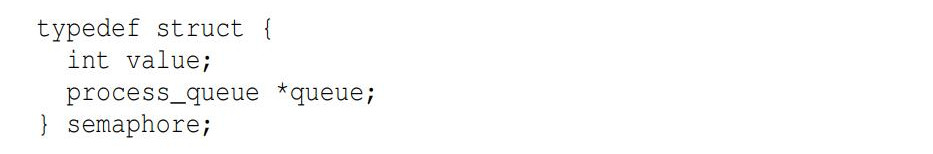
\includegraphics[width=\textwidth]{10.6_1.jpg}
    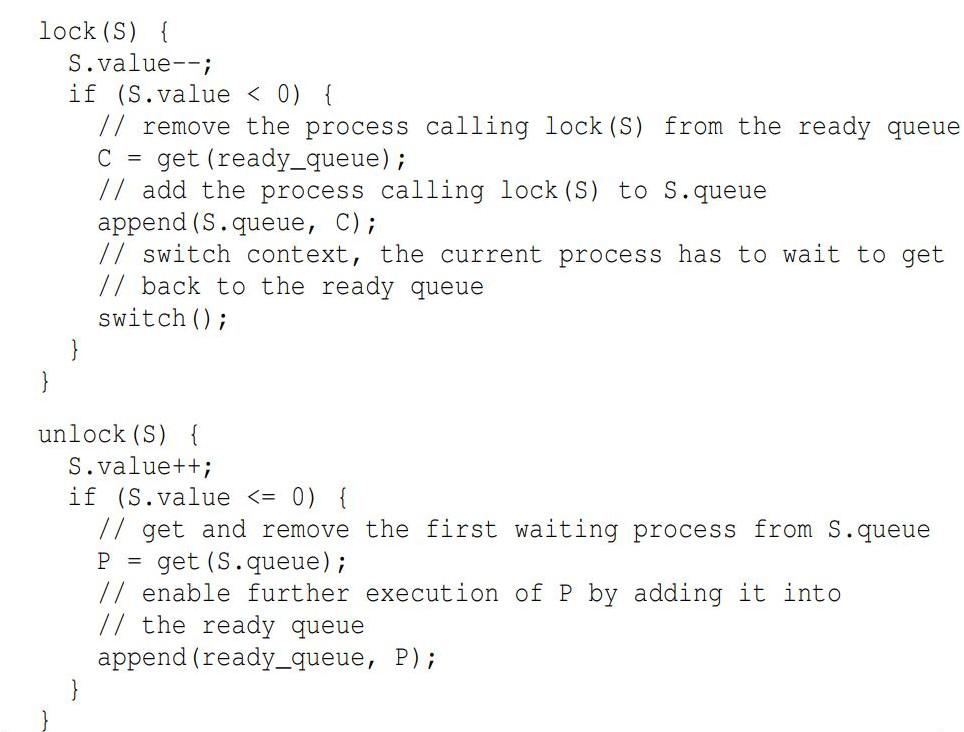
\includegraphics[width=\textwidth]{10.6_2.jpg}
    \caption{Z prezentace IOS: Synchronizace procesů -- kod implementace semaforu}
\end{figure}

\clearpage
\section{}
\textbf{Jedenáctá přednáška:} Pokračování a dokončení synchronizace procesů, monitory, deadlock.
 
\subsection{Monitory}
Synchronizační prostředky (ještě) vyšší úrovně (než semafory). Problém semaforů v reálném kódu je, že \textbf{je zde spousta sdílených dat, která se budou vzájemně vylučovat} -- nechceme mít celý program zamknutý -- bude zde snaha zamknutí minimalizovat -- může se stát, že se někde v nějaké větvi \textbf{zapomene lock/unlock a nastane problém} (v reálném kódu tak semafory jednoduché nejsou).
 
Proto vznikl komfortnější synchronizační mechanismus -- monitory. V syntaktické podobě vypadají takto (jazyk Ada, běžně se takto nepoužívají):
 
\begin{figure}[ht]
    \centering
    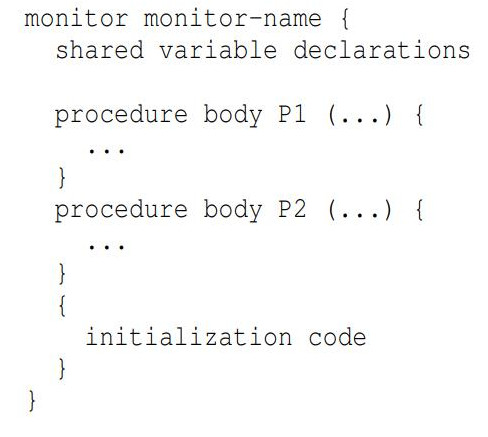
\includegraphics[scale=2]{11.1_1.jpg}
    \caption{Z prezentace IOS: Synchronizace procesů -- kód monitoru}
\end{figure}
 
\textbf{Monitor:}
\begin{itemize}
    \item je možné si představit jako datovou strukturu podobné třídě se sdílenými proměnnými,
    \item ty jsou sdíleny různými procesy pracující s monitorem,
    \item procesy se mohou k proměnným dostat přes procedury (metody monitoru),
    \item automatický monitor zajišťuje, že na něm v daném okamžiku poběží nejvýše 1 metoda,
    \item kdokoli chce pracovat se sdílenými zdroji, musí používat tyto metody, a tak se automaticky zajistí zamykání a odemykání zdrojů,
    \item použití -- do monitoru se nadefinují sdílené zdroje, dále mechanismy, jak se s nimi má pracovat (procedury), dále konstruktor (inicializační kód)
\end{itemize}

\newpage
\textbf{Popis monitoru:}
\begin{itemize}
    \item slupka (okraje) představují ochrannou bariéru monitoru,
    \item do monitoru je možné vstoupit definovanými operacemi (dveře),
    \item pokaždé, když do monitoru někdo vstoupí, tak se dveře uzamknou,
    \item další „zájemci o vstup“ jsou zařazení do čekací fronty vně monitoru (zařazování tím, že volají dané operace v okamžiku zamknutého monitoru),
    \item pokud se chtějí synchronizovat, použijí buď předdefinované podmínky programátorem, s každou z těch podmínek se pojí další čekací fronta (chci se sync pomocí podmínky x -- wait\_x() -- zařazení do fronty x -- současně bude vybrán někdo, kdo čeká na vstup monitoru a bude možnost v něm běžet -- já čekám ve frontě x na někoho, kdo se do monitoru dostane a provede \tcmd{signal} či \tcmd{notify} -- může mě uvolnit z fronty x)
\end{itemize}

\begin{figure} [h]
    \centering
    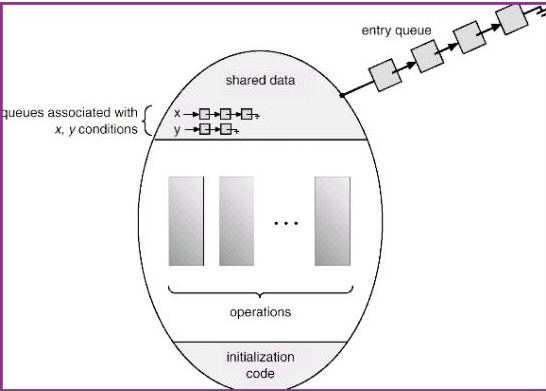
\includegraphics[scale=2]{11.1_2.jpg}
    \caption{Z prezentace IOS: Synchronizace procesů -- grafické ztvárnění monitoru}
\end{figure}

\textbf{Co když se procesy chtějí synchronizovat uvnitř monitoru?}
\begin{itemize}
    \item používá se mechanismus podmínek -- conditions,
    \item speciální datová struktura s definovanými operacemi nad ní, pomocí nich se procesy synchronizují,
    \item je možné volat \tcmd{wait()} -- synchronizovat se s někým na nějaké podmínce,
    \item je možné někomu, kdo na podmínce čeká, poslat uvolňující signál (operace \tcmd{signal()} nebo \tcmd{notify()})
\end{itemize}
 
\textbf{\tcmd{signal} a \tcmd{notify}:}
\begin{itemize}
    \item v monitoru může běžet jen jeden proces,
    \item pokud v něm jsou dva (z toho jeden ve frontě dané podmínky -- např. proces ve frontě x, druhý v monitoru a volá signal/notify):
    \begin{itemize}
        \item \tcmd{signal()} -- po zavolání pokračuje ten, kdo signál dostane (ten kdo je ve frontě, např. x) a běží v monitoru, druhý proces se buď zařadí do čekací fronty, nebo se zařadí do další fronty uvnitř monitoru, kde takovéto procesy čekají (a mají přednost před procesy ve frontě venku)
        \item \tcmd{notify()} -- po zavolání pokračuje volající, resp. ten, kdo signál dostal (ten, co byl ve frontě, se přesune buď do fronty mimo monitor, či do jiné fronty uvolněných, ale čekajících procesů)
    \end{itemize}
    
    \item čeká se, až bude proces odejde z monitoru nebo začne čekat (zařadí se do fronty podmínky)
    \item pokud nikdo na podmínce nečeká a někdo na ni použije \tcmd{signal} či \tcmd{notify}, jedná se o prázdnou operaci (nic se neprovede)
\end{itemize}

Monitory je možné implementovat \textbf{s využitím semaforu} (vstupní semafory, semafory ke každé podmínce, pro prioritní procesy -- pozastavené procesy ve frontě uvnitř monitoru). Monitory jsou dostupné v Javě či C\#. V POSIXu (C, C++, \ldots) jsou k dispozici alespoň podmínky (kombinace semaforů a podmínek) -- \tcmd{pthread\_cont\_t} a funkce \tcmd{pthread\_cond\_wait/signal/broadcast}.

\subsection{Některé klasické synchronizační problémy}
\subsubsection{Problém producenta a konzumenta}
\begin{itemize}
    \item máme smečku procesů, předem rozdělených, či se dynamicky dělí na producenty a konzumenty, komunikují spolu přes vyrovnávací paměť (např. pole s kruhovým bufferem),
    \item nutné procesy synchronizovat pro správnou práci s pamětí,
    \item řešením jsou tři semafory (full, empty, mutex),
    \item full -- říká, kolik položek je aktuálně v cache k dispozici, zamykáním si rezervují položku v paměti ke spotřebě,
    \item empty -- říká, kolik je volných slotů v cache, zamykáním se rezervuje kapacita pro zápis do cache,
    \item mutex -- pomocný semafor, který se zamkne při práci s ukazovátky do cache,
    \item \textbf{semafory je nutné vhodně inicializovat} (full=0, empty=max. hodnota cache, mutex=1)
\end{itemize}

\begin{figure}[ht]
    \centering
    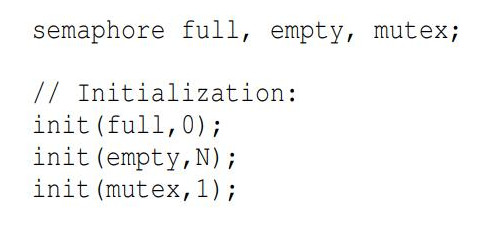
\includegraphics[scale=2]{11.2.1_1.jpg}
    \caption{Z prezentace IOS: Synchronizace procesů -- synchronizační prostředky producentů a konzumentů}
\end{figure}

\textbf{Pseudokód producenta:}
\begin{itemize}
    \item pracují tak, že vyprodukují položku, kterou chtějí zapsat do cache,
    \item nejprve zamknou empty (pokud se to podaří -- je tam volné místo a rezervují si ho pro sebe),
    \item zamknou mutex,
    \item začnou zapisovat do cache (posunou ukazovátko),
    \item odemkne se přístup do cache -- odemknutí mutex a full (konzumentům se dá najevo, že je zde položka ke konzumaci),
    \item pracuje v nekonečném cyklu \tcmd{do() \{\ldots\} while(1)}
\end{itemize}
 
\textbf{Pseudokod konzumenta:}
\begin{itemize}
    \item nejprve zamknou full (při úspěchu -- ve vyrovnávací paměti je něco ke konzumaci, položku si alokovali),
    \item zamknou si přístup k cache (zamkne se mutex),
    \item z vyrovnávací paměti se odstraní 1 položka,
    \item odemkne se přístup k cache (mutex) a následně se odemkne empty (dá se najevo producentům, že se v cache uvolnila položka),
    \item zkonzumuje se položka,
    \item pracuje v nekonečném cyklu \tcmd{do() \{\ldots\} while(1)}
\end{itemize}

\begin{figure} [h]
    \centering
    \scalebox{2}{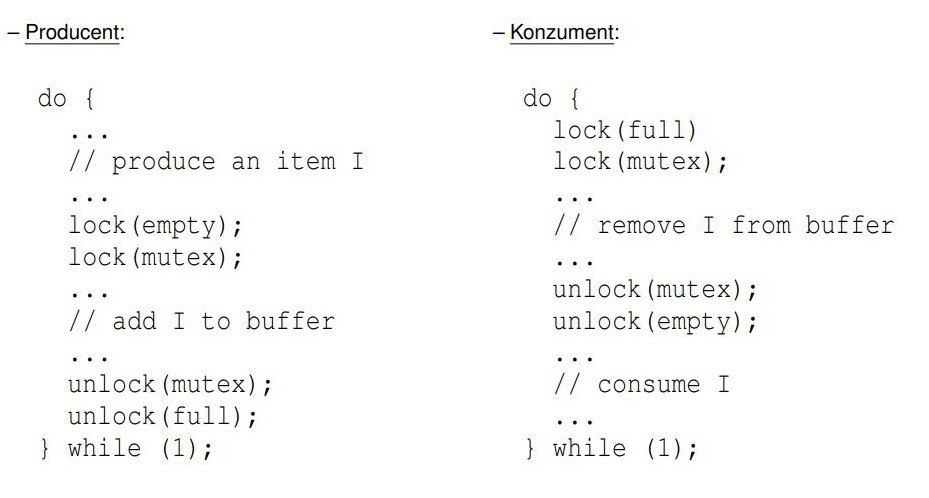
\includegraphics{11.2.1_2.jpg}}
    \caption{Z prezentace IOS: Synchronizace procesů -- pseudokód producenta a konzumenta}
\end{figure}

\newpage

\subsubsection{Problém čtenářů a písařů}
\begin{itemize}
    \item dva typy procesů -- čtenáři a písaři,
    \item pracují se sdílenou pamětí -- čtenáři ji mohou pouze číst, písaři jen měnit,
    \item může současně číst libovolný počet čtenářů (nemění se obsah paměti),
    \item pokud zapisuje nějaký písař, nesmí nikdo ani číst, ani psát,
    \item používá se sdílená proměnná readcount -- počet čtenářů,
    \item nutné použít semafor mutex (chránící přístup k readcount) a semafor wrt (semafor písařů),
    \item opět je nutná inicializace (počet čtenářů=0, oba semafory=1)
\end{itemize}

\begin{figure} [ht]
    \centering
    \scalebox{2}{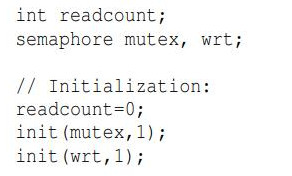
\includegraphics{11.2.2_1.jpg}}
    \caption{Z prezentace IOS: Synchronizace procesů -- synchronizační prostředky čtenářů a písařů}
\end{figure}

\textbf{Pseudokód písaře:}
\begin{itemize}
 \item pokud chce zapisovat, zamkne semafor wrt,
 \item až se mu to podaří, zapisuje,
 \item po dopsání odemkne wrt,
 \item pracuje v \tcmd{do() \{\ldots\} while(1)}
\end{itemize}

\textbf{Pseudokód čtenáře:}
\begin{itemize}
 \item v okamžiku, kdy chce číst, je nutné zamknout přístup k proměnné readcount (mutex), poté ji inkrementovat (zjistí tak, jestli je první),
 \item pokud readcount==1, tak se jedná o prvního čtenáře,
 \item potom se zamkne wrt a odemkne se mutex (readcount),
 \item začne číst (pokud přijde další čtenář, pouze readcount inkrementuje a čte),
 \item jakmile čtenář dočte, zamkne mutex,
 \item dekrementuje se readcount, pokd je ==0, znamená to, že je posledním čtenářem a musí odemknout přístup písařům (wrt),
 \item odemkne se přístup k readcount (mutex),
 \item pracuje v \tcmd{do() \{\ldots\} while(1)}
\end{itemize}

\begin{figure} [ht]
    \centering
    \scalebox{2}{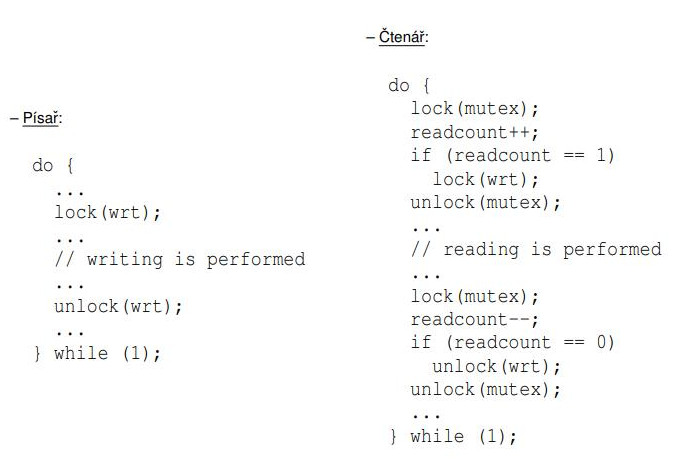
\includegraphics{11.2.2_2.jpg}}
    \caption{Z prezentace IOS: Synchronizace procesů -- pseudokód čtenářů a písařů}
\end{figure}

Toto řešení má nevýhodu -- \textbf{hrozí vyhladovění písařů} -- pokud do kritické sekce vejde 1 čtenář, přijde písař a začne čekat, přijde další čtenář, vejde do kritické sekce, první odejde, druhý taky, ale opět vejde první čtenář -- do nekonečna se tu střídají a písař nikdy nezapíše. Vyhladovění je někdy tolerováno, ale je dobré se mu vyhnout (malá pravděpodobnost, že se čtenáři budou do nekonečna střídat).
 
\textbf{Řešení vyhladovění:}
\begin{itemize}
    \item použije se další semafor -- wrt\_waiting -- čekající písař,
    \item písař nejprve zamkne wrt\_waiting, poté wrt, po zamknutí wrt odemkne wrt\_waiting,
    \item čtenáři na začátku provedou lock wrt\_waiting, unlock wrt\_waiting a poté pokračují dál (zajistí, že pokud nějaký písař začne čekat, tak všichni čtenáři dočtou, a po návratu na začátek nebudou schopni provést lock a unlock) \\
\end{itemize}

\subsubsection{Problém večeřících filozofů}
\begin{itemize}
    \item 5 filozofů, kteří reprezentují procesy,
    \item sesednou se kolem kulatého stolu, chtějí jíst a přemýšlet; jedí pomocí asijských hůlek, které budou mít rozděleny tak, že mezi každými filosofy je jedna hůlka, přičemž k jezení potřebují dvě -- 5 hůlek pro 5 filozofů,
    \item cyklus: získá si svojí levou a pravou hůlku, může se najíst, položí hůlky zpět, přemýšlí, poté opět jí,
    \item reprezentuje situaci, kdy mezi synchronizovanými procesy je cyklická závislost
\end{itemize}
 
\textbf{Možnost řešení:}
\begin{itemize}
    \item ne dokonalé řešení, možnost uváznutí (=špatné) a
    \item je možné, že dva filozofové budou jíst současně 1 hůlkou,
    \item zavede se 5 binárních semaforů (pole semaforů),
    \item všechny inicializované tak, že jsou odemknuté
\end{itemize}
 
\textbf{Filozof I:}
\begin{itemize}
    \item $i$ = ID, hodnota 0--4,
    \item zamkne hůlku $i$, následně zamkne hůlku $(i+1)\ mod\ 5$,
    \item pokud se podaří zámek obou hůlek, nají se,
    \item následně odemkne obě hůlky,
    \item může přemýšlet,
    \item \tcmd{do() \{\ldots\} while(1)}
\end{itemize}

\begin{figure} [htb]
    \centering
    \scalebox{1.6}{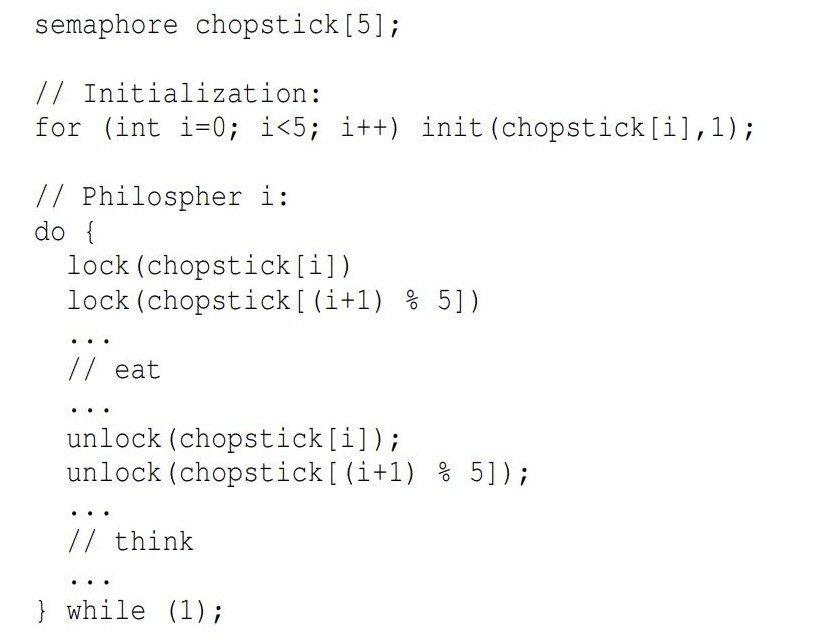
\includegraphics{11.2.3.jpg}}
    \caption{Z prezentace IOS: Synchronizace procesu -- pseudokód (špatného) řešení problému večeřících filozofů}
\end{figure}

\textbf{Gde deadlock?}
\begin{itemize}
    \item procesy se při plánování se mohou naskládat tak,
    \item že si každý vezme svou levou hůlku (každý hůlku se stejným číslem jako jeho ID),
    \item následně si každý z nich bude chtít získat tu druhou,
    \item každý bude trvat na tom, že si svoji nechá a chce tu druhou,
    \item celý systém se zastaví -- deadlock
\end{itemize}
 
\textbf{Řešení:}
\begin{itemize}
    \item jednou z možností je získávat obě hůlky současně,
    \item např. pomocí SysV semaforů, umožňují zamknout pole semaforů,
    \item další možností je získávat hůlky asymetricky -- alespoň 1 z filozofů bude brát hůlky v obráceném pořadí (např. každý lichý filozof bude brát hůlky nejprve $i$ a poté $(i+1)\ mod\ 5$ a sudí nejprve $(i+1)\ mod\ 5$ a potom $i$)
\end{itemize}

\subsection{Deadlock (uváznutí)} \label{deadlock}
\subsubsection{Definice}
\setstretch{1.3}
\textbf{Uváznutím (deadlockem) při přístupu ke zdrojům s výlučným (omezeným) přístupem rozumíme situaci, kdy \underline{každý} proces z určité \underline{neprázdné} množiny procesů je \underline{pozastaven} a čeká na uvolnění \underline{nějakého zdroje} s výlučným (omezeným) přístupem vlastněného \underline{nějakým procesem z dané množiny}, který \underline{jediný} může tento zdroj uvolnit, a to až \underline{po dokončení práce s ním}}.\vspace*{-1.5em}

\setstretch{1.1}
\begin{multline*}
  \exists \textcolor{orange}{P} \subseteq \mathds{P} : (\textcolor{orange}{P} \neq \emptyset \wedge \forall \textcolor{red}{p} \in \textcolor{orange}{P}\ (\text{pozastaven}(\textcolor{red}{p}) \wedge \exists \textcolor{blue}{r} \in \mathds{R} : (\text{čeká}(\textcolor{red}{p}, \textcolor{blue}{r})\ \wedge \\ \exists p' \in \textcolor{orange}{P} : (\text{vlastní}(p', \textcolor{blue}{r}) \wedge \text{uvolnitelný\_pouze\_vlastníkem\_po\_dokončení\_práce}(\textcolor{blue}{r})))))
\end{multline*}

\textbf{Vysvětlení definice:}
\begin{itemize}
    \item neprázdná množina procesů = \{1, 2, 1000, \ldots\}, aspoň jeden, ale ne nula! -- používáme tuto definici, jiné používají množinu procesů, kde jsou alespoň dva\footnote{Za deadlock se může považovat i situaci vzniklou při \emph{doublelockingu} -- self deadlock, proces zamkne zdroj a pak se jej pokusí zamknout ještě jednou.},
    \item výlučný přístup = zdroj, který používá v daném okamžiku nanejvýš 1 proces,
    \item omezený přístup = zobecněné kritické sekce, kde zdroj může používat určitý počet procesů, ale ne neomezený počet,
    \item pozastaven = není tam aktivní čekání, neběží (pokud to tam nebude, nebylo by možné rozlišit deadlock a livelock),
    \item zdroj vlastněný nějakým procesem z dané množiny = obvykle jiný, může to být i stejný proces,
    \item jediný \ldots po dokončení jeho použití = pracujeme s tím, že se používá zámek, který se používá neomezeně (žádný časový zámek), nikdo nemůže zdroj vzít, odemknout, nikde není žádný časovač
\end{itemize}

\textbf{Obecnější definice} (s možností uváznutí i bez prostředků s výlučným přístupem -- např. zasílání zpráv): \\
Uváznutím rozumíme situaci, kdy každý proces z nějaké neprázdné množiny procesů je pozastaven a čeká na nějakou událost, která by mohla nastat pouze tehdy, pokud by mohl pokračovat některý z procesů z dané množiny. (Je to např. situace, kdy proces 1 čeká na zprávu od procesu 2, ten čeká na zprávu od 3, 3 čeká na 4, \ldots proces 5 čeká na zprávu od 1.)

\subsubsection{Typický příklad deadlocku}
\begin{itemize}
    \item při přístupu ke zdrojům s výlučným omezeným přístupem,
    \item v praxi mohou být jednotlivá volání v kódu velmi daleko od sebe a zamykány mohou být jen za určitých podmínek,
    \item uváznutí se tak projeví jen zřídka a špatně se odhaluje a ladí
\end{itemize}

\newpage

\begin{figure} [htb]
    \centering
    \scalebox{2}{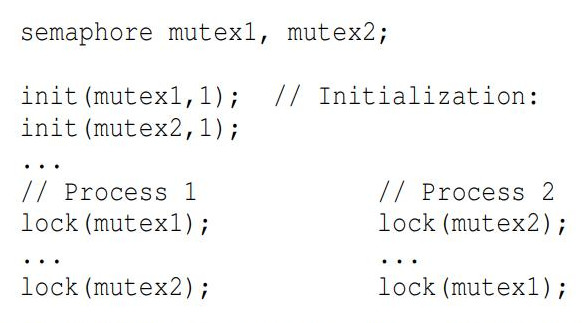
\includegraphics{11.3.jpg}}
    \caption{Z prezentace IOS: Synchronizace procesů -- příklad uváznutí}
\end{figure}

\textbf{Popis:}
\begin{itemize}
    \item dva semafory, oba na začátku odemknuté,
    \item za předpokladu použití standardních semaforů se standardní sémantikou, není zde jádro, které např. hlídá situaci a jeden z procesů by zabilo, \ldots
    \item jeden proces zamkne první mutex (semafor), něco provede, pokusí se zamknout druhý,
    \item druhý proces zamkne druhý mutex, něco provede a zamkne první,
    \item nastane deadlock
\end{itemize}

\subsubsection{Coffmanovy podmínky}

\textbf{K tomu, aby uváznutí nastalo (mohlo nastat), je nutné a postačující splnění čtyř podmínek:}
\begin{itemize}
    \item vzájemné vyloučení při používání prostředků,
    \item vlastnictví alespoň jednoho zdroje, pozastavení a čekání na další,
    \item prostředky může vrátit (pouze) ten proces, který je vlastní, a to po dokončení jejich využití (zdroj je vlastněn procesem, pouze ten proces ho může vrátit a to po dokončení využití toho zdroje),
    \item cyklická závislost na sebe (navzájem) čekajících procesů (rozumí se tím to, že jeden proces čeká na druhý -- žádné aktivní čekání v cyklu)
\end{itemize}

\subsubsection{Řešení uváznutí}
\begin{itemize}
    \item prevence uváznutí,
    \item vyhýbání se uváznutí,
    \item detekce a zotavení
\end{itemize}
 
Základní společná myšlenka všech řešení je \textbf{princip, kterým se snaží zrušit platnost alespoň jedné z nutných podmínek k uváznutí} -- když se jedna z Coffmanovych podmínek zneplatní, nemůže dojít k uváznutí.

\subsubsection{Prevence uváznutí}
\textbf{Řeší, jak tyto podmínky zneplatnit:}
\begin{itemize}
    \item první (vyloučení)
    \begin{itemize}
        \item nepoužívat žádné sdílené prostředky, nebo 
        \item užívat pouze takové sdílené prostředky, které umožňují skutečně současný sdílený přístup
        \item a u kterých není nutné vzájemné vyloučení procesu;
        \item ne vždy problém půjde vyřešit tímto způsobem.
    \end{itemize}
    
    \item druhá (vlastnictví)
    \begin{itemize}
        \item proces může žádat o prostředky pouze tehdy, pokud žádné nevlastní,
        \item (když chce proces používat současně 5 zdrojů v jednom okamžiku, musí zamknout všechny současně -- získá, nebo čeká -- systematicky v kódu zamykám všechny zdroje, nebo žádný zdroj -- kontrola zámku: pokud proces již něco zamkl, nemůže znovu zamykat -- musí vše uvolnit a teprve poté může zamknout),
        \item nevýhodou je nutnost zamknutí všech zdrojů, které se používají současně (např. 30 min se používá 1 zdroj, poté 1 min se používá další zdroj současně s prvním, ale musí se zamknout na 30 min oba zdroje),
    \end{itemize}
    
    \item třetí (návrat)
    \begin{itemize}
        \item nebudu vyžadovat, aby proces vždy získal všechny zdroje, které chce používat současně v 1 okamžik,
        \item ale umožním mu získávat postupně další a další zdroje, postupně přizamykat tyto zdroje,
        \item ale jen v situaci, kdy je opravdu možné tyto zdroje získat,
        \item pokud se proces pokusí něco přizamknout a ono se to nepovede, bude to řešeno speciálním způsobem
        \item (např. tak, že proces bude zabit a všechny zdroje mu budou odebrány),
        \item nevýhodou je situace, kdy v okamžiku, kdy se proces zabije, už mohl s některými zdroji něco dělat, zdroje mohou být v nekonzistentním stavu (ideálně se pokusit vrátit zdroje do konzistentního stavu),
    \end{itemize}
    
    \item čtvrtá (cyklická závislost)
    \begin{itemize}
        \item zavedením uspořádáním nad zdroji (očíslování),
        \item je možné tyto zdroje získávat pouze od určitého pořadí (např. od nejmenšího k největšímu -- začnu 1, pak 2, pak 3, \ldots -- pokud zamknu 5, můžu zamknout 5+, ale 3 už ne), 
        \item buď se konstrukcí programu zajistí, aby se vždy zamykalo v tomto pořadí, a poté analýzou, auditem se ověří, zda opravdu má program takovou zamykací disciplínu,
        \item anebo budu mít systém zamykání, který toto bude kontrolovat
    \end{itemize}
\end{itemize}

Ke všem bodům se dá říct, že buď bude program navrhován tak, aby byl konformní s použitou strategií, nebo se vynucení strategie kontrolovat až při běhu (což ale není jednoduché a spolehlivé).

\subsubsection{Vyhýbání se uváznutí}
Dalo by se to se chápat jako prevence 4. Coffmanovy podmínky. 

\textbf{Obecný princip:}
\begin{itemize}
    \item procesy musí předem deklarovat (jádru, systému správy zdrojů) informace o tom, jaké zdroje a jak budou používat, resp. které zdroje se budou používat a kolik jednotek zdroje se bude používat -- každý proces musí říct, kolik jednotek kterého zdroje bude používat (a další informace, např. „budu používat zdroje 1, 2, 3, 4, nikdy nebudu používat současně 1 a 2, apod.“),
    \item systém přidělování zdrojů si vede informace, co ty procesy deklarovaly,
    \item o jejich možných požadavcích,
    \item současně si vede informace o aktuálním stavu přidělování (ví, kdo co vlastní a kdo o co požádal),
    \item v okamžiku, kdy systém má neuspokojené žádosti, je uspokojí tehdy, pokud nemůže vzniknout žádná cyklická závislost na sebe čekajících procesů, ani v tom nejhorším možném případu, který by mohl nastat s ohledem na to, co procesy deklarovaly
\end{itemize}
 
\textbf{Příklad:}
\begin{itemize}
    \item situace v bance,
    \item od klientů mám svěřené peníze na termínované vklady, vím, kdy si klienti mohou své vklady vybrat,
    \item přijde někdo a bude chtít půjčku,
    \item je nutné se zamyslet, kolik zdrojů mám a kdy si to klienti mohou vybrat,
    \item půjčku mohu dát jen tehdy, když v nejhorším možném případě (všichni klienti si půjdou vybrat, co mohou) se nedostanu do dluhů
\end{itemize}

\textbf{Algoritmus založený na grafu alokace zdrojů:}
\begin{itemize}
    \item řeší problém vyhýbání se uváznutí,
    \item pouze systémy, kde má každý zdroj pouze jednu instanci,
    \item je veden systémem, který zdroje přiděluje, ten si průběžně udržuje graf vztahů mezi procesy a zdroji: dva typy uzlů (procesy a zdroje) a tři typy hran -- hrany od zdroje k procesu (který zdroj je kým vlastněn), hrany od procesu ke zdroji (kdo o který proces \emph{žádá} a kdo o který zdroj \emph{může požádat}),
    \item zdroj je přidělen pouze tehdy, pokud systém posoudí, že v budoucnu nemůže nastat cyklická závislost procesů, jednoduše tím, že „cvičně“ provede otočení žádostí na hranu vlastnictví (z P2 do R2 udělá R2 do P2), pokud v té situaci vznikne v grafu cyklus, znamená to, že v budoucnu by mohl vzniknout deadlock,
    \item v takovém okamžiku systém nepovolí přidělení zdroje (proces bude muset dál čekat na uvolnění zdroje, i když je volný)
\end{itemize}
 
Pokud by se používaly obecně zdroje se zobecněnou kapacitou, použil by se tzv. bankéřův algoritmus.

\subsubsection{Detekce uváznutí a zotavení z něj}
Systém přidělování zdrojů \textbf{umožní případný vznik uváznutí} (pokud pomineme to, že externě k množině uváznutých procesů máme \textit{strážného anděla}, který uváznutí vyřeší), \textbf{ale periodicky se detekuje, jestli k uváznutí nedošlo} (běží speciální proces, zajišťující, že nebude přebit prioritami jiných procesů), a pokud ano, provede se zotavení.
 
\textbf{Detekce uváznutí:}
\begin{itemize}
    \item vedení grafu vlastnictví zdrojů a čekání na zdroje (obdobný jako u vyhýbání se uváznutí) -- stejný počet uzlů, 2 typy hran (někdo žádá o zdroj, někdo vlastní zdroj),
    \item pokud vznikne v grafu cyklus, vím, že uváznutí nastalo
\end{itemize}
 
\textbf{Zotavení z uváznutí:}
\begin{itemize}
    \item alespoň některým procesům, které uvázly, odeberu zdroje,
    \item proces se buď zruší, nebo se pozastaví s tím, že může pokračovat, až bude moci získat všechny zdroje, které potřebuje,
    \item může nastat problém -- procesy zabiju, mohou mít ve zdrojích rozpracované nějaké operace -- zdroje mohou být v nekonzistentním stavu -- nutnost buď nechat systém uváznutý, nebo se spokojit s nekonzistencemi, nebo systém navrhnout tak, že při zabití procesu se nezabije ihned, ale prvně provede zotavení (rollback -- anuluje své operace a dostane zdroje do konzistentního stavu)
\end{itemize}

\subsection{Formální verifikace, verifikace s formálními kořeny}
Možnosti odhalování nežádoucího chování systému (uváznutí, stárnutí):
\begin{itemize}
    \item inspekce systému -- než se kód nasadí, kromě vývojáře kód musí projít i někdo další (či skupina), kteří schválí, že kód pochopili a je podle nich bezchybný,
    \item simulace, testování
    \begin{itemize}
        \item vestavěné systémy -- vytvoří si model systému a z něj se generuje kód, na modelu ověřují chování systému -- nevýhodou testování na jedné jednotce (modelu) je to, že se chyba nemusí projevit (nedeterminismus se nemusí projevit)
        
        \item paralelní programy -- vkládání šumu do plánování (na kritická místa před ně se vloží náhodná zpoždění, přepnutí kontextu), zvýší se tím množství proložených aktivit a šance, že se projeví nějaká chyba,
        
        \item dynamická analýza -- sleduje se, co se děje v systému, poté je snaha extrapolovat (=odhadovat), co by se mohlo stát,
        
        \item formální verifikace či verifikace s formálními kořeny -- pokud se řekne, že program nemá chybu či určitou vlastnost, tak ji má s platností matematického důkazu
    \end{itemize}
    
    \item obvykle se používají kombinace výše uvedených přístupů
\end{itemize}
 
Experimentuje se i s automatickými opravami -- je zde \textbf{běhový systém, který monitoruje, co se děje}; pokud uvidí, že nastala chyba, \textbf{pokusí se ji opravit automaticky} (např. sledování data race conditions: při porušení vzájemného vyloučení při přístupu ke sdílené proměnné se automaticky přidá zámek -- mohu ale tzv. pacienta zabít -- způsobit uváznutí, proto se například místo toho před prací s danou proměnnou místo vkládání zámku vynutí přepnutí kontextu -- zvýší se šance, že se projde kritickou sekci bez přepnutí kontextu)

\textbf{Proces formální verifikace:}
\begin{itemize}
    \item vytvoření modelu -- vytvoří se zdrojový kód či model, který se bude verifikovat (či kombinace, např. část jádra OS a model OS, odlehčená implementace),
    \item specifikace vlastností, které mají být ověřeny -- mohou to být generické vlastnosti, např. v systému nesmí být deadlock, nebo složitější vlastnosti, např. v cache není nikdy více než 10 položek,
    \item kontrola (automatická), zda model splňuje specifikaci
\end{itemize}
 
\textbf{Ověřování se provádí metodami:}
\begin{itemize}
    \item model checking (kontrola modelů),
    \item theorem proving (dokazování teorémů),
    \item static analysis (statická analýza)
\end{itemize}
 
Nad rámec verifikace se také provádí automatická analýza dle dané specifikace -- dodá se specifikace, jaké vlastnosti systém má mít, pro určité třídy systému je možné automaticky vysyntetizovat korektní implementaci.
 
\subsubsection{Theorem proving}
\begin{itemize}
 \item teorémem je zde věta, která říká: „Můj program XXX splňuje specifikaci YYY.“,
 \item používají se poloautomatické dokazovací prostředky (evidují, co už jste dokázali, mají databázi standardně platných skutečnosti z logiky, znají pravidla správného odvozování),
 \item vyžaduje se expert, který určuje, jak se důkaz má vést (přesto se to používá, např. mikrojádra ProvenCore či seL4),
 \item existují i plně automatické dokazovače (rozhodovací procedury, umí automaticky říct, zda platí, či ne) -- obvykle pro omezené fragmenty logik, spíše se používají jako pomocné
\end{itemize}

\subsubsection{Model checking}
\begin{itemize}
 \item obvykle plně automatizovaný přístup, prostředek,
 \item založen na systematickém generování stavu systému a stavového prostoru (systematicky se hledá, zda někde není chyba),
 \item nevýhodou je obrovský počet stavů -- např. při $N$ dvoustavových procesech (procesy začnou a skončí) může vygenerovat $2^N$ stavů -- problém stavové exploze
\end{itemize}

\subsubsection{Static analysis}
\begin{itemize}
 \item snaha analyzovat a verifikovat systém na základě jeho zdrojového kódu, aniž by se tento kód prováděl (nebo alespoň ne v původní sémantice -- např. celočíselné proměnné 0--1235, pamatuji si, jen jestli je hodnota záporná, 0, či kladná),
 \item nejjednodušší statický analyzátor je \tcmd{grep} (znají se syntaktické vzory chyb a grepem se vyhledávají),
 \item má různé podoby: data flow analysis, constraint analysis, type analysis, abstract interpretation, symbolic execution, \ldots
 \item nástroje: Facebook Infer, Frama-C, Microsoft SDV, SpotBugs, cppcheck, \ldots
\end{itemize}

\newpage

\section{}
\textbf{Dvanáctá přednáška:} Začátek správy paměti.
\subsection{Správa paměti}
Aby program mohl byt proveden, musí být spuštěn -- musí být nad ním vytvořen proces, musí mu být přidělen procesor a také paměť (a případně další zdroje -- soubory, \ldots).

\textbf{Rozlišujeme:}
\begin{itemize}
    \item logický adresový prostor -- LAP -- je virtuální adresový prostor, se kterým pracuje CPU při provádění kódu (uživatelského či jádra -- každý proces i jádro mají své logické adresové prostory),
    \item fyzický adresový prostor -- FAP -- adresový prostor fyzických adres paměti (obsahuje adresy, které se umisťují na adresové sběrnici, chceme-li z paměti načíst nebo do ní zapsat -- je společný pro všechny procesy i jádro)
\end{itemize}
 
Často logický adresový prostor \textbf{jádra bývá podprostorem logického adresového prostoru jednotlivých procesů}. Všechny logické adresové prostory procesu (v Linuxu) se překrývají ve stejné části -- \textbf{v části, kde je LAP jádra}. LAP jádra \textbf{není} procesům přístupný. Výhodou je, že při přechodu z režimu procesu na režim jádra se \textbf{pouze zpřístupní tento LAP} nebo při přepínání procesů (kromě změn mapování části LAP procesu) se \textbf{nemusí měnit mapování pro část LAP jádra}.
 
\textbf{Proces pracuje s logickými adresami, ale na adresovou sběrnici se umisťují fyzické adresy}. Toto mapování provádí \textbf{MMU (Memory Management Unit):}
\begin{itemize}
    \item HW jednotka specializovaná na překlad logických adres na fyzické, 
    \item dnes běžnou součástí čipu CPU,
    \item provádí překlad na základě datových struktur,
    \item obsah struktur je částečně uložen ve speciálních registrech, částečně v hlavní paměti systému,
    \item součástí MMU je cache, obvykle tzv. \textbf{TLB}, pro urychlení překladu
\end{itemize}
 
\textbf{Komunikace CPU a paměti:}
\begin{itemize}
    \item na CPU běží programy (CPU pracuje s logickými adresami),
    \item při čtení nebo zápisu z/na logickou adresu se adresa předá do MMU,
    \item MMU provede překlad logické adresy na fyzickou,
    \item MMU umístí fyzickou adresu na sběrnici a po ní se přenesou data mezi pamětí a CPU
\end{itemize}

\subsection{Přidělování paměti}
Existuje více úrovní přidělování paměti. V nejnižších (z hlediska blízkosti k HW) se přiděluje FAP pro zamapování do LAP; vyšší vrstvou je např. přidělování paměti přes knihovní funkce (\tcmd{malloc}, mimo režim jádra, či \tcmd{kmalloc}, \tcmd{vmalloc} v jádře); ještě na vyšší úrovni pak např. přidělování v rámci aplikací. 
 
Nejnižší úroveň přidělování je \textbf{implementována v jádře a jedná se o přidělování FAP pro zamapování LAP}. Běžné způsoby přidělování paměti (a mapování LAP na FAP):
\begin{itemize}
    \item přidělování po spojitých blocích (contiguous memory allocation),
    \item segmentech,
    \item stránkách,
    \item kombinace výše uvedeného (Intel -- segmenty a stránky)
\end{itemize}
 
\newpage
\textbf{Funkce malloc:}
\begin{itemize}
    \item při žádosti o alokaci nějakého kusu paměti (počtu bajtů)
    \item musí malloc požádat jádro o přidělení FAP,
    \item požaduje od jádra větší blok paměti (segment, stránka),
    \item z bloku paměti se vykousne požadovaný počet bajtů,
    \item ty dostane k dispozici uživatel,
    \item při volání dalších mallocu, dokud požadovaný počet bajtů nebude větší než přidělený blok, nepůjdou požadavky do jádra, ale bude se čerpat již přidělený prostor
\end{itemize}

\subsection{Contiguous Memory Allocation}
Mechanismus mapování logických adres na fyzické a přidělování paměti po spojitých blocích. Jedná se o \textbf{nejjednodušší mechanismus jak z hlediska HW, tak obsluhy OS}. V běžných výpočetních systémech se příliš \textbf{nepoužívá}, nicméně je vhodný pro jednoduché a vestavěné aplikace, které mají běžet na jednoduchém HW.
 
\textbf{Popis:}
\begin{itemize}
    \item je to po spojitých blocích (něco jako spojité ukládání dat),
    \item k popisu takového mapování je třeba znát, ve kterém FAP je zamapován počátek LAP,
    \item je nutné vědět, jak je úsek paměti velký (pro odchycení přístupu mimo meze tohoto prostoru)
\end{itemize}
 
\textbf{Překlad adresy:}
\begin{itemize}
    \item MMU si pro aktuálně běžící proces pamatuje 2 údaje,
    \item v limitním registru si pamatuje, kolik proces paměti dostal,
    \item v relokačním registru si pamatuje, na jakou fyzickou adresu byl zamapován LAP procesů,
    \item když dostane logickou adresu,
    \item zjistí, zda je adresa v rámci naalokovaného prostoru,
    \item pokud ne -- chyba při přístupu do paměti, pošle se přerušení typu trap, obvykle je proces předčasně ukončen,
    \item pokud ano -- mapování se provede tak, že se použije bázová adresa, na kterou je zamapován FAP procesů, sečte se s logickou adresou prostoru = mám adresu ve FAP (fyzickou adresu)
\end{itemize}
 
\textbf{Příklad překladu LA na FA:}
\begin{itemize}
    \item proces 1 má začátek LAP na začátku FAP (konec na FAP 100 000), proces 2 někde uprostřed (LA 0 = FA 1 mil.),
    \item překlad LA 10 procesu 1,
    \item zkontroluje se, zda 10 je menší než 100 000 (= konec LAP procesu 1),
    \item bázová adresa 0 se přičte s LA, tedy 0 + 10 = 10,
    \item překlad LA 10 procesu 2,
    \item zkontroluje se, zda 10 je v rámci rozmezí (ano),
    \item bázová adresa 1 000 000 se přičte k 10, tedy 1 000 010
\end{itemize}
 
\textbf{Tento mechanismus má řadu nevýhod:}
\begin{itemize}
    \item výrazně se zde projevuje externí fragmentace paměti (FAP),
    \item přidělováním a uvolňováním úseků paměti vzniká posloupnost obsazených a neobsazených úseku paměti, úseky mohou být obsazeny různými procesy,
    \item nejhorším dopadem je, že při sčítání volných úseků paměti může být prostor pro přidělení paměti procesu dostatečný, ale tyto volné úseky nejsou (nemusí být) spojité, takže zde zdánlivě není dostatek paměti pro daný proces (není možné provést alokaci),
    \item problémy se zvětšováním prostoru daného procesu,
    \item snaha o minimalizace dopadů externí fragmentace pomocí různých strategií (first fit se nepoužívá, namísto toho například best fit, worst fit či binary buddy, \ldots),
    \item provádí se dynamická reorganizace paměti (nákladné)
    \item není možné rozumně řídit přístupová práva v rámci přidělené paměti (nelze: část paměti pro čtení, část pro zápis, \ldots),
    \item není možné také sdílet část adresového prostoru (vše nebo nic),
    \item při virtualizaci paměti (swapování) je nutné odložit veškerou paměť na disk a poté ji vrátit zpět -- pomalé, může být zbytečné.
\end{itemize}

\subsection*{Definice:}
\begin{description}
\item[bázová adresa] -- počátek LAP (tj. adresa 0 v LAP) ve FAP (nebo: počáteční adresa LAP procesů ve FAP)

\item[first fit] -- prochází se volnými úseky a použije se první volný úsek

\item[best fit] -- podívám se na seznam volných úseků a vybere se ten, který je dostatečně velký, ale vyberu ten nejmenší z dostatečně velkých

\item[worst fit] -- paradoxně lepší jak best fit, opak best fit, hledá se úsek dostatečně velký a použije se ten největší (zbyde nepoužitý velký kus, který se využije později, např. při dalším zvětšování)

\item[binary buddy] -- udržuje se seznam volných úseků paměti, najdu si úsek paměti, který odpovídá nejlépe, a pokud přesahuje, resp. je 2x větší než požaduji, rozdělím ho na polovinu a opět zjistím, zda je úsek 2x větší, pokud ano, dělím úseky tak dlouho, až dojdu k úseku paměti, který nelze rozdělit na poloviny tak, aby byl uspokojen daný požadavek, a paměť se přidělí
\end{description}

\subsection{Segmentace paměti}
\begin{itemize}
    \item LAP je rozdělen na kolekci segmentů,
    \item segmenty mohou být přiděleny překladačem/programátorem jednotlivým částem procesu (částem dat, procedurám, zásobníku, \ldots),
    \item každý segment má číslo a velikost,
    \item LA je číslo segmentu a posun v něm,
    \item jednotlivé segmenty patřící jednomu procesu nemusí být zamapovány spojitě (jeden segment bude zamapován spojitě, ale různé segmenty nemusí)
\end{itemize}
 
\textbf{Překlad adresy LA na FA:}
\begin{itemize}
    \item MMU potřebuje pracovat s tabulkou segmentů, která je uložená v RAM -- v MMU je odkaz na začátek tabulky (= pole),
    \item logická adresa je dělena na číslo segmentu $s$ a posuv v rámci segmentu $d$ (displacement),
    \item při překladu se vezme číslo segmentu $s$, např. při práci s $s=10$ se podívá do řádku tabulky 10,
    \item na příslušném řádku se najde, jakou má segment velikost, jakou má bázovou adresu,
    \item pokud bude např. $d=1000$, podívá se, jestli je d v rámci paměťového prostoru, který je přidělen,
    \item pokud ne -- výjimka, chyba,
    \item pokud ano -- vezme se bázová adresa segmentu, sečte se to s posuvem a mám FA
\end{itemize}

\textbf{Příklad překladu:}
\begin{itemize}
    \item mám LA se segmentem $s=10$ a posuvem $d=1000$,
    \item přistoupím na 10. řádek tabulky segmentu,
    \item zde budu mít limit (velikost segmentu, zde např. 100 000) a jeho bázi (odpovídající počáteční adresu ve FAP),
    \item pokud $d$ je v limitu (1000 < 100 000?),
    \item vezmu bázi (např. 1 000 000), sečtu ji s $d$,
    \item tzn. 1 000 000 + 1000 a dostanu fyzickou adresu (1 001 000)
\end{itemize}

\textbf{Výhody:}
\begin{itemize}
 \item mohou být použity jako jemnější jednotka ochrany při přístupu do paměti (některé mohou označeny jako pro čtení, některé pro zápis, některé v režimu jádra, \ldots),
 \item jemnější jednotka pro odkládání paměti na disk (odložit se mohou segmenty, ne celá paměť procesu),
 \item jemnější jednotka pro sdílení,
 \item implementace je jednoduchá,
 \item paměť je přidělována nespojitě, zmírňují se dopad externí fragmentace
\end{itemize}

\textbf{Nevýhody:}
\begin{itemize}
 \item při zvětšování opět dopad externí fragmentace,
 \item možný zdroj chyb, segmentace je viditelná procesu
\end{itemize}

\subsection{Stránkování}
Je aktuálně nejpoužívanějším mechanismem mapování LAP na FAP. LAP je rozdělen na \textbf{jednotky pevné velikosti -- stránky}, FAP je rozdělen na odpovídající \textbf{jednotky stejné velikosti -- rámce}. (Nejčastěji bývá velikost stránky 4~KiB.)
 
\subsubsection{Vlastnosti}
\textbf{Výhody:}
\begin{itemize}
    \item paměť je přidělována po rámcích (ty se zamapují do stránek),
    \item neviditelné pro uživatelské procesy,
    \item minimalizují se problémy s externí fragmentaci (podobně jako clustery u disků):
    \begin{itemize}
        \item pořád vznikají úseky volných a využitých, nicméně nejmenší nevyužitá „díra“ v paměti je 1 rámec, ten se vždy dá využít (nespojité přidělování paměti),

        \item je snaha přidělovat paměti po spojitých posloupnostech rámců (pokud je to možné), např. pomocí algoritmu binary buddy
    \end{itemize}
    \item jemná jednotka ochrany přístupu do paměti (každá jednotlivá stránka může být r, rw, v uživatelském režimu či v režimu jádra, NX bit -- jestli je možné obsah stránky spouštět jako kód),
    \item jemná jednotka sdílení (paměť sdílená mezi procesy lze sdílet pro stránkách),
    \item při nedostatku paměti se odkládá po jednotlivých stránkách
\end{itemize}
 
\textbf{Nevýhody:}
\begin{itemize}
    \item složitější implementace,
    \item větší režie,
    \item interní fragmentace (podobně jako u disků),
    \item možné snížení rychlosti přístupu do paměti -- nespojitá alokace, projeví se větším počtem kolizí v caches,
    \item zpomalování alokace a dealokace paměti (delší práce se strukturami, které popisují aktuální obsah paměti),
    \item jsou vnímány jako výrazně menší než výhody systému -- proto jsou používány nejvíce
\end{itemize}

\subsubsection{Mapování logických adres na fyzické}
V nejjednodušším případě se používají \textbf{jednoduché -- jednoúrovňové tabulky stránek}. OS udržuje \textbf{informaci o volných rámcích} (záleží na OS, HW nezajímá), pro každý \textbf{proces si udržuje tabulku stránek} (musí být strukturovaná tak, aby tomu daná architektura rozuměla).
 
\subsubsection{Tabulky stránek}
\begin{itemize}
    \item logická adresa je rozdělena na číslo stránky ($p$ -- place) a na posuv stránky ($d$ -- displacement),
    \item číslo stránky se použije jako index do tabulky stránek (= pole v paměti),
    \item v MMU je registr, který bude ukazovat na to, kde má daný proces uloženou tabulku stránek,
    \item číslo stránky se vezme jako index do tabulky stránek ($p=10 \Rightarrow$ přistoupím na 10. položku),
    \item pokud byla stránka alokována (= má přidělen rámec), na daném řádku najdu číslo rámce,
    \item číslo rámce se spojí s posuvem a dostanu FA
\end{itemize}
 
Na řádku tabulky stránek, který odpovídá dané stránce, kde je uloženo odpovídající číslo rámce, \textbf{jsou uložené řídicí příznaky mapování -- platnosti mapování, přístupů, modifikace, přístupová práva} (r, rw, user režim, jádro režim, možnost provádění), \textbf{globality}.
 
Tabulky stránek jsou udržovány v \textbf{hlavní paměti (RAM)}, \textbf{zvlášť} pro každý proces, MMU mají ve speciálním registru \textbf{pouze ukazatel na začátek tabulky stránek}, při přepínání kontextu se \textbf{mění pouze ukazatel} na začátek tabulky stránek. (Konkrétně u Intelu se ten registr jmenuje \emph{CR3}.)
 
Neprovedeme-li žádnou další optimalizaci, tak každý jednotlivý přístup do paměti (pro data či instrukce) se změní \textbf{z jednoho přístupu na 2} (při načtení dat z RAM -- nejprve musím jít do tabulky stránek, poté načíst vlastní data -- obojí jsou v RAM) -- zpomalení o 100 procent. Používá se tak \textbf{vyrovnávací paměť TLB -- Translation Look-aside Buffer} pro urychlení práce s pamětí.

\textbf{Příklad překladu LA na FA:}
\begin{itemize}
    \item LA, tvořená číslem stránky $p=10$, posuvem $d=1000$,
    \item MMU bude mít v paměti umístěnou tabulku stránek, v registru bude odkaz na adresu, kde se nachází tabulka stránek,
    \item MMU použije $p=10$ jako index do tabulky stránek, přistoupí na řádek 10 tabulky stránek,
    \item součástí obsahu řádku je odpovídající číslo rámce (např. 500),
    \item dostaneme fyzickou adresu, tvořena rámcem $f=500$ a posuvem $d=1000$
\end{itemize}

\subsection*{Definice:}
\begin{description}
\item[příznak platnosti mapování] --  zda daný adresový blok je, nebo není použit (ne všechny tabulky stránek v daném okamžiku musí být využity)

\item[příznak přístupu] -- byla stránka od okamžiku zavedení paměti zpřístupněna? (dále slouží jako informace, zda je stránka vhodná na odložení do paměti -- jádro čas od času prochází bity a přístupové bity nuluje, při hledání kandidáta na odložení se zjišťuje, zda v několika periodách bylo ke stránce přistoupeno nebo ne -- pokud delší dobu ne, bude odložena)

\item[příznak modifikace] -- byla, nebo nebyla stránka modifikována? (Při odložení stránky a poté znovuzavedení do paměti -- aby se nemodifikovaná stránka neodložila znovu.)

\item[příznak globality] -- když je stránka globální, je sdílená za běhu různých procesů, typicky se používá pro stránky jádra
\end{description}

\subsubsection{TLB}
\begin{itemize}
    \item obsahuje dvojice číslo stránky a číslo rámce + jsou tam některé řídicí příznaky spojené s mapováním (oprávnění, modifikace),
    \item v TLB nejsou celé stránky či rámce -- je to cache pro mapování čísla stránky na číslo rámce),
    \item typicky implementovaná jako (částečně) asociativní paměť,
\end{itemize}
 
\textbf{Někdy je operace částečně asociativní:}
\begin{itemize}
    \item několik bytů z LA je použito klasickým způsobem adresování,
    \item zbytek je použit pro asociativní vyhledávání,
    \item např. pokud se vymezí pro klasické adresování 2 byty, TLB se rozdělí na 4 části/bloky (00,01,10,11), v rámci bloku se bude hledat asociativně
\end{itemize}

\textbf{Překlad:}
\begin{itemize}
    \item obdobně jako bez TLB,
    \item místo přístupu do paměti na určitý řádek tabulky bude HW hledat, zda někde v TLB je položka s číslem 10 a pokud ano, vezme k tomu odpovídající číslo rámce,
    \item pokud takové vyhledání nastane, říká se tomu TLB hit, použije se okamžitý překlad -- číslo rámce a posuv a jsem v FAP,
    \item pokud se nepodaří úspěšně vyhledat položku, použije se stejný postup jako bez TLB (přes paměť) -- TLB miss
\end{itemize}
 
\textbf{Příklad překladu s TLB:}
\begin{itemize}
    \item architektura s jednoúrovňovou tabulkou stránek, k dispozici TLB, který je částečně asociativní, 2 bity se použijí pro rozlišení částí TLB a zbytek se prohledává asociativně,
    \item LA, rozdělená na číslo stránky $p$ -- to na rozděleno na horní 2 bity (adresování v rámci TLB), zbytek bude číslo stránky (p=01 a zbytek 10), posuv $d=1\ 000$,
    \item TLB rozděleno na 4 bloky, jeden z nich adresován bity 00, další 01, další 10, a poslední 11,
    \item p=01 10 mi říká, že mám jíst do 2. části,
    \item v bloku budou čísla stránek, odpovídající rámce,
    \item všechny řádky se prohledají paralelně -- je v některém z těch řádků číslo 10 ?,
    \item ano -- vezmu odpovídající rámec (např. 1 000 000) -- TLB hit,
    \item FA bude $f=1\ 000\ 000$ a posuv $d=1\ 000$,
    \item ne -- nastane TLB miss, je nutné jít do klasické tabulky stránek a tam hledat
\end{itemize}

K neúspěšnému vyhledání může dojít \textbf{při přístupu k instrukčnímu kódu} (čtení instrukce, operandů), \textbf{u každého čtení může dojít k neúspěšnému vyhledání opakovaně} (např. 32b architektura, 4B instrukce, nesprávně zarovnaná instrukce, 2 B na začátku 1. stránky, 2 B na začátku 2. stránky -- je nutné provést překlad čísel na odpovídající rámec u obou stránek -- může dojít 2x k TLB miss) -- pro instrukci velkou 4 B, která načítá 4 B z paměti, jsou nutné 4 překlady a $4\times$ může nastat TLB miss.

\textbf{Pokud dojde k TLB miss:}
\begin{itemize}
 \item HW bude hledat automaticky v tabulce stránek -- platí u architektur, kde je TLB  řízený hardwarem (většina architektur),
 \item jsou i softwarově řízené TLB; pokud nastane TLB miss, nastane přerušení od MMU k CPU, jádro si tento překlad provede, specializovanými instrukcemi se naplní překlad do TLB a překlad adresy se opakuje (CPU jako MIPS, SPARC)
\end{itemize}

Někdy může být použito více TLB, např. 64b architektury obvykle mají překlad náročnější -- je potřeba více TLB (např. dvouúrovňová TLB -- jedna pro překlad kódových adres, druhá pro adresy dat).

\textbf{Při přepnutí kontextu} (mění se hodnota ukazatele tabulky stránek v MMU registru) \textbf{je nutné invalidovat obsah TLB a znovu naplnit jej naplnit; používají se optimalizace:}
\begin{itemize}
 \item používají se globální stránky (stránky používané jádrem -- jsou na stejném místě),
 \item na některých CPU se ještě do řádku TLB doplňuje identifikátor procesu, pro který je mapování platné (vyhledává se na základě čísla procesů a čísla stránky),
 \item při změnu obsahu tabulek stránek je také nutná invalidace obsahu TLB (neprojevily by se změny v tabulce stránek)
\end{itemize}

Údaje se do (HW řízených) TLB dostávají tak, že \textbf{se překlad nahrává do TLB při prvním přístupu na stránku}, při nedostatku překladů se nějaký překlad odstraní. HW také \textbf{počítá s tím, že budeme s pamětí pracovat spojitě}, tak si může někdy nahrát do TLB překlady následujících adres \textbf{dopředu}. \textbf{V případě SW řízených TLB může být obsah nahráván speciálními instrukcemi jádrem}.

\subsection*{Definice:}
\begin{description}
\item[asociativní paměť] -- také obsahem adresovatelná paměť; nefunguje jako pole, vyhledává podle (části) obsahu paralelním porovnáváním se všemi položkami
\end{description}

\subsubsection{Efektivita stránkování s TLB}
Efektivní přístupová doba je:

$$(\tau + \epsilon) \alpha + (2 \tau + \epsilon)(1 - \alpha)$$

\begin{itemize}
    \item kde $\tau$ je vybavovací doba RAM,
    \item $\epsilon$ je vybavovacídoba TLB,
    \item $\alpha$ je pravděpodobnost úspěšného vyhledání v TLB (TLB hit ratio, $1 - \alpha$ je tedy pravděpodobnost neúspěchu),
    \item jedna se vážený průměr, kde se spočítá doba přístupu do paměti, pokud se zadaří vyhledání $(\tau + \epsilon) \alpha$,
    \item pokud se nezadaří vyhledání, počítá se doba \emph{dvou} přístupů do paměti $2\tau + \epsilon$
\end{itemize}

Tento vztah je sestaven za předpokladu, že poté, co se neúspěšně vyhledá v TLB, půjdu do RAM, najdu překlad v RAM, a poté půjdu do RAM pro data -- v praxi to funguje tak, že pokud \textbf{MMU nalezne překlad v RAM, automaticky ho ihned doplní do TLB, provede opakovaný překlad pro TLB, a až poté jde pro data do paměti}. (V praxi by přístupová doba při TLB miss byla $2\tau + 2\epsilon + \delta$, kde $\delta$ je čas pro provedení úpravy TLB.)
 
Je \textbf{důležité, aby bylo vyhledávání TLB úspěšné, jinak se přístupová doba do paměti bude výrazně zpomalovat}. Úspěšnost TLB ovlivňuje:
\begin{itemize}
    \item velikost TLB (to ovlivní výrobce čipu),
    \item dobrá lokalita odkazů programu (může ovlivnit programátor)
\end{itemize}
 
\textbf{Příklad:}
\begin{itemize}
    \item inicializace čtvercové matice, NxN prvků,
    \item v paměti linearizována, ukládají se typicky \emph{po řádcích},
    \item inicializace 2 způsoby,
    \item první způsob inicializuje matici po sloupcích, druhý po řádcích,
    \item v případě přístupu po řádcích je v souladu s uložením paměti po řádcích -- bude výrazně efektivnější z hlediska možného počtu neúspěšného vyhledání TLB; přístup po sloupcích bude méně efektivní,
    \item v případě TLB s jednou položkou a 2x2 matice, kde prvek zabírá půlku stránky, nastane při přístupu po řádcích 2x TLB miss, po sloupcích nastane 4x TLB miss
\end{itemize}
 
\subsection*{Definice:}
\begin{description}
\item[lokalita odkazů] udává, s kolika různými shluky adres (adresy blízko sebe, shluk = 1 stránka) pracuje v daném procesu za krátký časový okamžik program (pokud shluků adres není mnoho, program má dobrou lokalitu adres)
\end{description}

\subsubsection{Implementace tabulek stránek}
Kdyby se tabulky stránek implementovaly jako jednoúrovňové, zabraly by příliš moc paměti. 

Pro 32b systémy (Intel) se stránkami o velikosti 4 KiB (12 bitů se odkousne na posuv stránky), zbývá 20 bitů LA, udávají číslo stránky a počet řádků v tabulce stránek (odpovídá počtu stránek), odpovídá to >1 milionu položek. Má-li mít 1 položka tabulky stránek 4~B (je tam číslo stránky, rámce -- 20 bitové, k tomu řídicí příznaky -- celkem potřeba 27 bitů + zarovnání na bajty -- 32 bitů), dostáváme tak 4~MiB pro jednu tabulku stránek pro každý proces (běžně může běžet 100 procesů -- jen na tabulky stránek by bylo potřeba 400~MiB)
 
Pro 64b systémy je problém ještě horší -- také se používají 4KiB stránky, teoreticky by šlo použít až 52 bitů na adresu stránky -- pro položku bude potřeba 8~B.
 
\subsubsection{Hierarchické tabulky stránek}
Nebude zde 1 tabulka stránek pro 1 proces, ale pro \textbf{1 proces bude více tabulek v hierarchické struktuře}, ne všechny dílčí tabulky musí být v daném okamžiku alokované (vznikají \textit{tabulky tabulek tabulek\ldots stránek}).
 
\textbf{Princip fungování} hierarchické tabulky na příkladu \textbf{dvouúrovňové tabulky stránek (používané u i386)}:
\begin{itemize}
    \item 32b logická adresa, 12 dolních bitů je vymezeno na posuv v rámci stránky ($2^{12}$ = 4KiB velikost stránky),
    \item zbývajících 20 bitů je pro číslo stránky (rozděleno na horní a dolní část po 10b), používají se jako indexy do dílčí tabulky stránek 2. úrovně a následné dílčí tabulky stránek 1. úrovně,
    \item dílčí tabulka 2. úrovně je pro daný proces právě jedna -- označuje se jako \emph{adresář stránek},
    \item v registru CR3 (v MMU na Intelu) je uložen odkaz na začátek adresáře stránek (= tabulka 2. úrovně, forma pole) pro aktuálně běžící proces,
    \item první úroveň tabulek stránek nemusí být použita příslušným příznakem v adresáři stránek (je možné říct, že příslušná položka adresáře stránek nepoužívá 1. úroveň -- pracujeme s velkými stránkami -- zde s posuvem 22 bitů = 4MiB stránky)
\end{itemize}

\textbf{Překlad LA na FA (na příkladu výše):}
\begin{itemize}
    \item vezme se obsah tech horních 10 bitů (31--22), je to 10b číslo, které se použije jako \emph{index} do adresáře stránek (tabulky 2. úrovně),
    \item index = číslo řádku,
    \item na této položce najdu \emph{odkaz, čili adresu} začátku dílčí tabulky stránek 1. úrovně (těch může být víc),
    \item vezmu číslo uložené v dalších 10 bitech (21--12), použiju ho opět jako index do této tabulky,
    \item zde bude odpovídající číslo rámce,
    \item za předpokladu, že v části, kde jsou řídicí příznaky, je uvedeno, že mapování je platné,
    \item číslo rámce se vezme, přidá se k tomu posuv a mám FA
\end{itemize}

\textbf{Efektivita přístupu do paměti dvouúrovňové tabulky stránek:}
\begin{itemize}
    \item z jednoho přístupu se stanou 3 přístupy,
    \item nejprve musím do adresáře stránek (první přístup),
    \item poté do dílčí tabulky stránek (druhý přístup),
    \item až poté mohu do paměti (třetí přístup),
    \item pokud nebude pracovat TLB, zpomalení bude o 200 procent
\end{itemize}
 
\textbf{Tabulky stránek na x86-64 systémech (čtyřúrovňové tabulky):}
\begin{itemize}
    \item 64 bitové adresy, dvouúrovňové tabulky stránek nestačí,
    \item dolních 12 bitů je použito jako offset stránky ($\Rightarrow$ 4KiB stránky),
    \item číslo stránky má (47--12) 36 bitů,
    \item tedy máme 48 bitů logické adresy (+ je vyžadováno znaménkové rozšíření do 64 bitů, bit 47 se tedy musí opakovat až po bit 63),
    \item číslo stránky je rozděleno na 4 indexy (odspodu po 9 bitech index do 1. úrovně, 2. úrovně, 3., 4.),
    \item 1. úrovni se říká \emph{dílčí tabulka stránek} (page table, PT),
    \item 2. úrovni se říká \emph{adresář stránek} (page-directory table, PD),
    \item 3. úroveň je \emph{tabulka ukazatelů} (page-directory-pointer table, PDP),
    \item 4. úroveň žádné extra jméno nemá (page-map-level-4 table, PML4)
\end{itemize}

\textbf{Překlad LA na FA ve čtyřúrovňové tabulce stránek na x86-64 systémech:}
\begin{itemize}
    \item opět se používá registr CR3, ve kterém je uložen odkaz na začátek tabulky 4. úrovně. Adresa PML4 je v CR3 uložená mezi bity 51--12, protože fyzické adresy mohou mít maximálně 52 bitů (limit architektury) a PML4 má velikost jedné stránky ($2^{12}$ B, 4~KiB), spodních 12 bitů se tak používá na indexaci v ní,
    \item mezi bity 47--39 se vezme index do tabulky 4. úrovně, tam se najde odkaz na začátek tabulky 3. úrovně,    
    \item použije se další index (bity 38--30), dostaneme odkaz na začátek tabulky 2. úrovně, 
    \item použije se poslední index (20--12), dostaneme odkaz na dílčí tabulku stránek, tam dostaneme číslo rámce, k němu se přičte posuv,
    \item dostáváme fyzickou adresu,
    \item jeden řádek v tabulce zabírá zde 8~B, při 4KiB tabulce na adresaci jednoho řádku stačí 9 bitů (proto tady 9, ne 10 jako u 32b)
\end{itemize}
 
V x86-64 dojde \textbf{bez TLB ke zpomalení o 400 procent} -- 5 přístupů do paměti. Konečná adresa nemusí být nutně až v poslední PT, s použitím nějakých příznaků je opět možné adresovat „velké stránky“, pak může být adresování:
\begin{itemize}
    \item čtyřúrovňové -- stránky o velikosti 4 KiB,
    \item tříúrovňové -- stránky velké 2 MiB,
    \item dvouúrovňové -- stránky velké 1 GiB (u některých procesorů)
\end{itemize}
 
\subsubsection{Hierarchické tabulky stránek a TLB}
Při použití hierarchických tabulek stránek zásadně \textbf{roste význam TLB}:

\begin{itemize}
    \item na 64b CPU jsou větší, mají složitější organizaci,
    \item mají víceúrovňové TLB, bývá oddělena zvlášť pro datové stránky a instrukční stránky (i7 -- dvě úrovně TLB, zvlášť je úroveň datová a instrukční, poté je společná TLB úrovně 2)
\end{itemize}

\newpage
Další možnosti \textbf{optimalizace práce s TLB:}
\begin{itemize}
    \item globální stránky -- stránky jádra, které jsou sdílené mezi jednotlivými procesy, jsou označené jako globální a nemusí se vyhazovat při přepnutí kontextu,
    \item vstupy TLB spojené s identifikátory procesů -- kromě čísla stránky, rámce bude na jednotlivých řádcích TLB také ID procesu,
    \item používá se spekulativní dopředné nahrávání překladu TLB,
    \item používají se specializované cache (kromě TLB) pro ukládání položek (úrovní) tabulek stránek
\end{itemize}
 
\textbf{Zanořené hierarchické tabulky stránek (Intel/AMD):}
\begin{itemize}
    \item při virtualizaci vznikají zanořené tabulky stránek (tabulky stránek host OS, tabulky stránek virtuálního OS),
    \item v případě 64b procesorů se bude používat 8 úrovní tabulek stránek (4 pro VM, další 4 pro hosta),
    \item používá se tak odlišení položek v TLB používané na fyzickém stroji pro různé virtuální stromy -- je zde identifikátor pro virtuální PC (VPID na Intelu nebo ASID na AMD)
\end{itemize}
 
\subsubsection{Příklad na čtyřúrovňové tabulce stránek}
Chci provést 8B instrukci, která bude načítat 8 B z paměti. \textbf{Kolik přístupů do paměti se v nejhorším případě provede?}
\begin{itemize}
    \item instrukce a data mohou být na jiných stránkách, oboje samostatně mohou být na rozmezí 2 stránek (4 B 1. stránka, 4 B 2.), navíc každou stránku nemusím mít fyzicky v prostoru za sebou (nelze to načíst jedním čtením -- čtu že 2 rámců),
    \item jen pro načtení instrukce a dat budou potřeba 4 přístupy do paměti (pouze jde o samotné čtení instrukce a dat! -- nutný ještě překlad),
    \item překlad se provádí pro každou stránku zvlášť přes 4úrovňovou tabulku stránek,
    \item provádět se budou $4\cdot4$ přístupy (4 stránky, 4 úrovně) pro překlad adres, tzn. dalších 16 přístupů,
    \item celkem tak $16 + 4 = 20$ přístupů do paměti
\end{itemize}

\subsubsection{Hashované tabulky stránek}
\begin{itemize}
    \item logická adresa členěna na číslo stránky $p$, posuv stránky $d$,
    \item MMU si vede překladovou tabulku, která má charakter \emph{hash tabulky}, ve speciálním registru bude odkaz na začátek hash tabulky,
    \item vezme se číslo stránky, prožene se hashovací funkci (ta je implementována v HW, MMU) -- vypadne odkaz do hashovací tabulky (číslo řádku hash tabulky),
    \item problém -- více různých stránek se může namapovat na stejnou položku v hashovací tabulce,
    \item není zde tak přímo umístěn překlad, ale odkaz na zřetězený seznam překladových položek (číslo stránky, rámce), 
    \item tento seznam MMU musí projít a dohledat případný překlad,
    \item až najdeme odpovídající položku, najdeme rámec, ten umístíme do adresy místo čísla stránky, přidá se posuv -- dostaneme FA,
    \item efektivita závisí na délce zřetězených seznamů -- pokud bude hash funkce špatná, efektivita bude špatná.
\end{itemize}

\subsubsection{Modifikace hashovaných tabulek stránek}
\begin{itemize}
    \item nemusí se používat celé číslo stránky pro hashování,
    \item je možné použít jen několik bitů stránek pro rozlišení různých hashovacích tabulek
\end{itemize}

\textbf{Fixní počet překladových položek:}
\begin{itemize}
    \item zřetězený seznam překladových položek bývá nahrazen fixním počtem překladových položek, které se ukládají do hashovací tabulky na daný řádek (namísto aby v tabulce byl odkaz na seznam, tabulka bude „širší“ a na 1 řádku bude 4--8 překladových položek a hledá se v rámci řádku),
    \item pokud překlad nebude nalezen, neznamená to, že stránka není mapována, pouze se pošle přerušení, jádro zjistí, že se nepodařilo dohledat na daném řádku, proto musí jít do tabulek stránek, které si vede ve vlastní režii (SW tabulka stránek),
    \item zde si dohledá, jestli překlad existuje (pokud ne, nastane \emph{výpadek stránky}),
    \item pokud existuje, upraví se tabulka stránek tak, aby tam dané číslo bylo,
    \item používá se např. u CPU PowerPC nebo na CPU Itanium (položky mohou být zřetězeny, ale HW zřetězený seznam nepoužívá -- pokud je první položka překlad, použije se, pokud ne -- přerušení, jádro se podívá, jestli má nějaký další seznam překladových položek a čistě v SW se dohledá překlad, pokud ho najde, provede se úprava tabulky stránek a nový překlad)
\end{itemize}
 
\textbf{Může být sdílena všemi procesy:}
\begin{itemize}
    \item je nutné do překladových položek umisťovat číslo stránky, ale i odpovídající číslo procesu,
    \item hashovací funkcí se prožene číslo stránky i číslo procesu,
    \item dohledává se tak dle čísla stránky i procesu,
    \item namísto čísla procesu se může ještě pracovat s čísly paměťového regionu, každý proces má svá čísla regionu, lokální čísla regionu se mapují na čísla globální -- umožňuje sdílení regionů (lokální regiony procesu se můžou namapovat na 1 fyzický region -- sdílený), adresa je dána číslem regionu a číslem stránky,
    \item kromě čísla stránky mám ještě lokální region v LA, region se převede na globální číslo regionu, číslo stránky se prožene hash funkcí a bude se vyhledávat -- používá se u PowerPC a Itanium
\end{itemize}
 
\subsection*{Definice:}
\begin{description}
\item[paměťové regiony] -- LAP je dělen na stránky a na vyšší úrovni je dělen na regiony -- skupiny stránek, které následují za sebou, jsou proměnné velikosti (něco jako extenty), jsou použity za určitým účelem (datový, kódový, \ldots)
\end{description}

\subsubsection{Příklad na sdílené hashovací tabulce stránek s regiony}
LAP je rozdělen na stránky, ty jsou \textbf{děleny na regiony} (např. 6 stránek -- region 1 má první 3 stránky, region 2 ostatní),
\begin{itemize}
    \item LA = lok. číslo regionu, číslo stránky, posuv v rámci stránky,
    \item lokální číslo regionu se přeloží přes tabulku na globální číslo regionů, to se spojí s číslem stránky,
    \item posuv se nemění,
    \item glob. číslo regionu a číslo stránky se prožene hashovací funkci,
    \item dostanu odkaz do hash tabulky, na určitý řádek,
    \item rozdělena na určitý (pevný) počet záznamů, 
    \item vždy je tam číslo regionu, číslo stránky, odpovídající rámec, potom další číslo regionu, stránky, rámec atd.,
    \item prohledávám, jestli se někde v příslušné položce nachází dvojice globální číslo regionu a číslo stránky,
    \item k tomu najdu odpovídající rámec
\end{itemize}

\subsubsection{Invertovaná tabulka stránek}
\begin{itemize}
    \item nepřekládá číslo stránek na číslo rámce, ale obráceně -- číslo rámce na číslo stránky,
    \item mapuje rámce na stránky,
    \item její řádky odpovídají rámcům, je zde tolik položek, kolik mám rámců,
    \item tabulka je nutné sdílená -- pro všechny procesy,
    \item je to pole,
    \item hashování je řešené hardwarově
\end{itemize}
 
\textbf{Překlad:}
\begin{itemize}
    \item v položkách tabulky se kromě čísla stránky ukládá i PID procesu,
    \item vezmu PID, číslo stránky,
    \item prohledávám \emph{od začátku do konce},
    \item zjišťuji, jestli některý řádek odpovídá PID a stránce, které mě zajímá,
    \item nalezl jsem překlad,
    \item odpovídající rámec má hodnotu $i$, kde $i$ je řádek tabulky, na kterém jsem odpovídající překlad našel.
\end{itemize}
 
\textbf{Výhody:}
\begin{itemize}
    \item úspora paměti (1 tabulka pro všechny)
\end{itemize}
 
\textbf{Nevýhody:}
\begin{itemize}
    \item prohledávání od začátku do konce je neakceptovatelné -- příliš pomalé -- řeší se kombinaci s hashováním,
    \item není moc používaná,
    \item komplikace s tím, jak implementovat sdílení stránek -- pokud více procesů bude sdílet nějaký rámec, stejné položce bude odpovídat více dvojic PID a číslo stránky, jenže může zde být jen jedna dvojice -- neustále bude docházet k výpadkům,
    \item jádro si musí (paralelně) tak vést klasické tabulky stránek, těmi projde, zjistí že překlad je možný, opraví ho, bude chtít první překlad a jedna položka se bude vyhazovat,
    \item ještě kromě stránek jsou zde regiony, indexovat se pomocí čísla regionu a čísla stránky
\end{itemize}

\textbf{Kombinace s hashováním:}
\begin{itemize}
    \item místo hledání od začátku do konce,
    \item se vezme PID a číslo stránky, proženu hashovací funkci,
    \item dostanu odkaz do tabulky,
    \item prohledávám od tohoto místa,
    \item typicky je uvnitř tabulky zřetězení
\end{itemize}
 
\subsubsection{Příklad na invertované tabulce stránek s hashováním}
\begin{itemize}
    \item mám PID procesu, jeho LA = číslo stránky a posuv v rámci stránky,
    \item vezmu PID a číslo stránky, proženu hashovací funkci,
    \item dostanu odkaz na nějaký řádek invertované tabulky stránek (v MMU je odkaz na začátek),
    \item na daném řádku bude uloženo, pro jaký proces je mapování, pro jakou stránku je mapování, a odkaz na další stránku procesu,
    \item pokud PID a číslo stránky nesouhlasí s daným řádkem, je zde odkaz na jiný řádek, kde má daný proces jinou stránku,
    \item pokud najdu odpovídající PID a číslo stránky,
    \item nalezli jsme odpovídající rámec,
    \item číslo rámce je číslo položky -- řádek v tabulce
\end{itemize}

\newpage

\section{}
\textbf{Třináctá přednáška:} Dokončení správy paměti.
\subsection{Virtualizace paměti}
\textbf{PAE -- page address extension} -- Intel, rozšíření na $2^{36}$ bitů fyzické adresy, kde 4 horní bity nastavoval OS. To umožnilo \textbf{využít až 64~GiB paměti na 32b systémech} (z hlediska procesu ale bylo možné použít maximálně 4~GiB).
 
Virtualizace paměti umožňuje procesu a jádru pracovat \textbf{s oddělenými lineárními logickými adresovými prostory}. Každý proces vidí svůj prostor, mezi sebou nekolidují. Pro jednotlivé procesy jsou přístupy \textbf{transparentní -- neví o tom, že v jeden okamžik část používaného FAP využívá např. jiný proces}.
 
Výhodou je \textbf{mensi spotřeba paměti, rychlejší odkládání na disk, zavádění do paměti} (není nutné odložit či zavést celý adresový prostor procesu).
 
Část paměti \textbf{lze odložit na disk a v případě potřeby opět nahrát do PC}. Z disku se části LAP zavádí do FAP pouze tehdy, pokud je to nutné.
 
Hovoříme pak o:
\begin{itemize}
    \item stránkování na žádost,
    \item segmentování na žádost.
\end{itemize}
 
\subsection{Stránkování na žádost} \label{strankovani-na-zadost}
Stránky \textbf{jsou zaváděny do paměti, jen pokud k nim přistupujeme}. OS uchovává informace o tom, které stránky jsou využité, a které ne (resp. v tabulce stránek udržuje bit, který určuje, jestli je stránka v paměti, nebo na disku).
 
Pokud po vyhledání čísla stránky (a příslušného rámce) \textbf{je stránka uložena v paměti}, postupuje se normálně (přeloží se na FA). Pokud ne, \textbf{pošle se přerušení OS (trap) -- jedná se o výpadek stránky} (page fault).
 
U jiných tabulek stránek (hash, invertovaných) se HW podívá do seznamu stránek, pokud tam stránka nebude, OS se podívá ještě do svých SW tabulek stránek. Pokud však zjistí, že se přistupuje na LA, která není namapována v paměti, dojde k \textbf{výpadku stránky}.
 
Výpadek stránky \textbf{je přerušení od MMU, které udává, že nelze převést adresu}, čili že není definováno mapování v tabulce stránek.
 
\subsection{Obsluha výpadku stránky}
\begin{itemize}
    \item kontrola, zda proces neodkazuje mimo přidělený adresový prostor (pokud ano, \textbf{segfault}, jádro proces ukončí),
    \item alokace rámce,
    
    \begin{itemize}
        \item proces přistupuje do paměti, která není v FA namapovaná,
        \item použije se volný rámec, pokud nějaký volný je,
        \item pokud není, vybereme si stránku v paměti, která má již přidělený rámec (\emph{victim page} -- oběť), odložíme oběť na disk (pokud byla stránka změněna), uvolníme rámec a použijeme uvolněný rámec 
    \end{itemize}
    
    \item inicializace stránky (po alokaci závislá na předchozím stavu stránky),
    \begin{itemize}
        \item pokud jde o první odkaz na stránku: pokud je to kód či inicializovaná data, načte se z programu, u všech ostatních se data \textbf{vynulují} (kvůli bezpečnosti),
        \item pokud to nebyl první přístup (stránka už byla v minulosti uvolněna z FAP): pokud to je kód či konstantní data, načtou se z programu, ostatní: pokud byla modifikovaná, ze swapu se stránka vrátí zpět do FAP, jinak se obsah opět vynuluje
    \end{itemize}
    
    \item úprava tabulky stránek -- upravit odkaz, kam vede LA (rámec se změní),
    \item proces je připraven na opakováni instrukce, která výpadek způsobila (je ve stavu připravený)
\end{itemize}

\subsection{Výkonnost stránkování na žádost}
Efektivní doba přístupu do paměti:
$$(1 - p)T + pD$$

\begin{itemize}
    \item kde $p$ je \emph{page fault rate} = pravděpodobnost výpadku stránky; $(1 - p)$ je pravděpodobnost, že k výpadku nedojde,
    \item $T$ doba přístup bez výpadku,
    \item $D$ doba přístup s výpadkem.
\end{itemize}

Doba přístupu bez výpadků je mnohem menší než doba přístupu s výpadkem. Závisí na \textbf{dostatku paměti a přiměřeném počtu procesů, lokalitě odkazů v procesech, vhodném výběru zaváděných či odkládaných stránek} (algoritmus výběru „oběti“) -- snaha mít $p$ co nejmenší.

\subsection{Počet výpadků stránek}
Máme 1 instrukci, kolik výpadků při jejím zpracování může nastat? Může k němu dojít při \textbf{čtení instrukce, při práci s každým z jejích operandů}, u obou může dojít k výpadku \textbf{vícenásobně}.
 
Vícenásobné výpadky mohou být způsobeny:
\begin{itemize}
    \item nezarovnáním instrukce (půlka instrukce v 1. stránce, druhá půlka ve 2. stránce),
    \item nezarovnáním dat (jako instrukce výše),
    \item data jsou delší než 1 stránka (instrukce pracující s mnoho daty, např. na Intelu MOVSB),
    \item výpadky tabulek stránek na různých úrovních -- např. hierarchická tabulka stránek, kdy tabulky mohou být velké, proto se odkládají do paměti a může opět docházet k výpadkům -- obvykle alespoň část tabulek stránek je chráněna před výpadkem stránek (zejména tabulka stránek nejvyšší úrovně)
\end{itemize}

\textbf{Příklad (podobný bude u zkoušky):}

Jaký je maximální počet výpadků stránek v systému se stránkami o velikosti 4~KiB, čtyřúrovňovou tabulkou stránek, u které pouze dílčí tabulka nejvyšší úrovně je chráněna proti výpadku, při provádění nenačtené instrukce o délce 4 B, která přesouvá 8~KiB z jedné adresy paměti na jinou?
\begin{itemize}
    \item instrukce bude na rozmezí dvou stránek
    \begin{itemize}
    \item při přístupu na 1 stránku je nutné projít celou hierarchickou tabulku stránek (máme 4 úrovně, 1 chráněná),
    \item v tab 1. úrovně je odkaz na tab. 2. úrovně, zde k výpadku může dojít (+1), tu je odkaz na tab 3. úrovně (+1), stejně u 4. úrovně (+1), to, kam ukazuje tab. 4. úrovně (na FAP) opět nemusí být v paměti (+1),
    \item pro zpracování 1. části instrukce může dojít ke 4 výpadkům stránek,
    \item zpracování 2. části: 1. stránka bude úplně na konci všech tabulek stránek -- při inkrementaci se musí
    \item načíst úplně nové 4 úrovně tabulek stránek -- opět může dojít k 4 výpadkům jako předtím,
    \item celkem 4 + 4 = 8 výpadků po načtení instrukce
    \end{itemize}
    \item instrukce se musí spustit, přesouvá 8~KiB dat (při 4~KiB stránkách), 
    \begin{itemize}
        \item nejhorší případ: zdrojová data o velikosti 8~KiB jsou rozložena na 3 stránkách (2~KiB první stránka, 4~KiB druhá, 2~KiB třetí),
    \item cílová data budou na tom obdobně,
    \item abych dostal první stránku zdroje, může opět dojít ke 4 výpadkům,
    \item při práci s druhou stránkou -- opět první je na konci seznamu, tedy +1 bude úplně v jiných tabulkách -- další +4 výpadky,
    \item poslední stránka -- protože LA následují za sebou, první dvě stránky byly na rozmezí (konec -- začátek tabulek), nyní bude ve stejných tabulkách stránek jako předchozí -- tedy +1 výpadku stránek (je možný pouze výpadek na úrovni rámce)
    \item celkem +9 výpadků
    \item u cíle úplně stejný případ jako u zdroje, tedy +9 výpadků,
    \item provádění instrukce zabere 9 + 9 = 18 výpadků,
    \end{itemize}
    
    \item tedy dohromady při vykonání jedné této instrukce může dojít celkem k 8 + 18 = 26 výpadkům stránek (maximální možný počet, nejhorší případ)
\end{itemize}

\subsection{Odkládání stránek}
K tomuto může dojít při výpadku stránky. Může být odložení:
\begin{itemize}
    \item lokální -- v rámci procesu (u kterého došlo k výpadku),
    \item globální -- bez ohledu na to, kterému procesu patří která stránka.
\end{itemize}
 
Typicky je neustále udržován \textbf{určitý počet volných rámců}:
\begin{itemize}
    \item pokud počet volných rámců klesne pod určitou mez, aktivuje se page daemon (zloděj stránek), který běží tak dlouho, dokud neuvolní dostatečný počet stránek,
    \item při výpadku stránky se použije rámec z množiny volných rámců,
    \item lze doplnit heuristikou, která uvolené stránky okamžitě nepřiděluje, ale zjišťuje, jestli nebyla vybraná oběť, která není správná
\end{itemize}

\subsection{Algoritmy výběru odkládaných stránek (obětí)}

\subsubsection{FIFO}
\begin{itemize}
    \item \emph{first in, first out},
    \item odstraňuje stránku, která byla zavedena do paměti před nejdelší dobou (a nebyla dosud odstraněna),
    \item např. proces pracuje se 4 stránkami (1, 2, 3, 4), chce pátou, není dost paměti -- uvolní se stránka 1, rámec, kde byla 1, se použije pro 5,
    \item výhody -- jednoduchá implementace,
    \item problémy:
    \begin{itemize}
        \item může odstranit starou stránku, která se ale často používá,
        \item trpí \emph{Beladyho anomálii} -- očekáváme, že v systému, ve kterém často dochází k odkládání a zvětší se paměť systému, tak k odkládání bude docházet méně často -- to zde pravda být nemusí -- počet výpadků vzroste při zvětšení paměti,
    \end{itemize}
    \item dá se trochu změnit -- omezit problém s odstraňováním starých, ale používaných rámců: umístíme takový rámec do množiny volných rámců, přidělíme jiný volný rámec, pokud bychom chtěli rámec použit, ihned se získá tento uvolněný rámec (signál -- špatná oběť, vybere se jiná), pokud ne, odloží se
\end{itemize}
 
\subsubsection{LRU}
\begin{itemize}
    \item \emph{least recently used},
    \item snaží se odkládat nejdéle nepoužitou stránku,
    \item dobrá aproximace hypotetického ideálního algoritmu (znal by budoucnost a podle požadavků z budoucnosti by rozhodoval, co aktuálně odložit tak, aby byl počet výpadků minimální -- zatím to nejde)
    \item problémy:
    \begin{itemize}
        \item při cyklických průchodech polí se algoritmus může chovat velmi neefektivně -- např. systém se 4 rámci, dělám bubble sort na 5 paměťových blocích (první 4 bloky budou na všech rámcích, zpracují poslední, první vyhodím a dám na první rámec, poté potřebují něco pro první blok, vyhodím druhý rámec, \ldots pořád dokola)
    \item řeší se to například strategii odstranění naposledy použité stránky (MRU -- \emph{most recently used})
    \item další problém je problematická implementace -- je nutné umět detekovat použitou stránku (nutná HW podpora, např. časové razítko)
    \end{itemize}
    \item používají se aproximace LRU
\end{itemize}
 
Aproximace LRU \textbf{pomoci omezené historie referenčního bitu stránek} (page aging):
\begin{itemize}
    \item použije se jeden bit -- referenční bít,
    \item tento bit HW nastaví na 1 při každém přístupu,
    \item jádro si vede omezenou historii tohoto bitu (pro jednotlivé stránky),
    \item periodicky se posouvá obsah historie doprava (shiftuje se referenční bit doprava),
    \item poté se referenční bit v tabulce stránek vynuluje,
    \item poté při výběru obětí jádro projde všechny historie a vybere z nich nejmenší hodnotu (zn. používala se stránka před nejdelší dobou)
\end{itemize}
 
Aproximace LRU \textbf{algoritmem druhé šance}:
\begin{itemize}
    \item stránky jsou uloženy v kruhovém seznamu,
    \item máme jeden ukazatel, tím seznam procházíme,
    \item vynulujeme referenční bit dané stránky,
    \item pokud už bude 0, použijeme danou stránku jako oběť,
    \item také se tomu říká clock algorithm \\
\end{itemize}
 
\textbf{Modifikace algoritmu druhé šance:}
\begin{itemize}
    \item upřednostňují se jako oběti nemodifikované stránky (ušetří se 1 zápis na disk) -- modifikované se zapíší na disk a dostanou další šanci,
    \item dva ukazatele, které prostupují frontou -- jeden nuluje referenční bit, druhý odstraňuje oběti (double-handed clock algorithm),
    \item Linux:
    \begin{itemize}
        \item fronty aktivních a neaktivních stránek -- pokud nějaká stránka je během 1 periody zpřístupněna $2\times$, tak se přesune do fronty aktivních stránek, pokud ne, přehodí se do fronty neaktivních stránek (z té se vybírají oběti),
    \item systém se snaží odkládat stránky, které jsou použité jako různé vyrovnávací paměti
    \item pokud má proces namapován určitý počet stránek, OS se snaží odstraňovat jeho neaktivní stránky,
    \item odkládání se provádí po určitých počtech (najednou), čím více je paměť zaplněna, tím více se rámců uvolní,
    \item je možné nastavit procesu příznak, aby se jeho stránky neodkládaly (nebyly oběti),
    \item při kritickém nedostatku paměti jádro ukončuje některé procesy (většinou: pokud dojde RAM i swap zároveň) -- obvykle to ale bývá příliš pozdě,
    \item v Linuxu existuje služba EarlyOOM (není služba jádra!) -- začne tyto procesy ukončovat dřív při nedostatku paměti
    \end{itemize}
\end{itemize}

\subsection{Alokace rámců procesům (resp. jádru)}
\begin{itemize}
    \item důležité hlavně u lokálního výběru,
    \item u globálního výběru lze použít pro řízení výběru obětí,
    \item je třeba mít vždy přidělen minimální počet rámců pro provedení jedné instrukce -- jinak dojde k nekonečnému vyměňování stránek potřebných k provedení instrukce,
    \item dále se používají různé heuristiky pro určení počtu rámců pro procesy:
    \begin{itemize}
        \item podle velikost programu, priority, objemu fyzické paměti, \ldots,
        \item na základě pracovní množiny stránek -- množina stránek, které používá proces za nějakou určitou dobu (aproximace pomocí referenčního bitu),
        \item sledování frekvence výpadku procesu (více výpadků, častěji $\Rightarrow$ proces dostane více fyzické paměti)
    \end{itemize}
\end{itemize}
 
Přidělování rámců \textbf{s využitím pracovní množiny, kombinace lokální a globální výměny, využívá např. Windows}:
\begin{itemize}
    \item procesy a jádro mají jistý minimální a maximální počet rámců,
    \item pokud je dost paměti, rámce se jim dodávají až do dosažení maxima (může se i zvětšit),
    \item pokud se dosáhne maxima a není dost paměti, provede se lokální výměna,
    \item pokud je volných rámců výrazný nedostatek, OS začne procházet běžící procesy a začne jim odebírat určitý počet stránek na základě omezené historie přístupů,
    \item při výběru obětí se dává přednost procesům běžícím méně často,
    \item snaží se vyhýbat těm procesům, které běží na popředí, a těm procesům, které měly v poslední době mnoho výpadků,
    \item počáteční pracovní meze se zjistí při startu systému dle velikosti fyzické paměti,
    \item při odkládání na disk vybrané oběti jí dá ještě 2. šanci -- nechá si ji ještě chvíli v paměti, přidělí jí jiný rámec, aby bylo možné korigovat chyby při volbách oběti,
    \item umí swapovat všechna data procesu na disk (typicky dlouho neaktivní proces)
\end{itemize}

\subsection{Trashing}
Trashing je problém, který může nastat při odkládání stránek na disk. Vznikne, pokud máme \textbf{systém s vysokou mírou paralelismu} (resp. mnoho spuštěných procesů) -- procesy potřebují nějaký \textbf{minimální počet rámců, se kterými musí pracovat}. Pokud je počet procesů velký, paměti \textbf{je málo a často může docházet k odkládání na disk}. Potom může dojít k tomu, že \textbf{proces stráví více času náhradou stránek než užitečným výpočtem}.

Občas v nějakých OS existuje \textbf{swapper} (služba OS), ten pozastaví některé procesy a odloží veškerou paměť na disk. Možností je také ukončit některé procesy.
 
\subsection{Poznámky}
\textbf{Prepaging} -- do fyzické paměti zavádí více stránek zároveň (start procesu, po odswapováni, \ldots -- zrychlení).
 
\textbf{Zamykání stránek:}
\begin{itemize}
    \item zabraňuje se odložení,
    \item užívá se např. u stránek, do nichž probíhá I/O (stránky se mohou mapovat do zařízení -- nechceme tyto stránky ukládat na disk), u (části) tabulek stránek (např. nejvyšší úroveň), u (některých) stránek jádra, na přání uživatele (např. v paměti pracujeme s citlivými daty)
\end{itemize}

\textbf{Sdílení stránek}
Dá se sdílet:
\begin{itemize}
    \item kód programu (proces vícekrát spuštěný, není třeba mít stejný kód v paměti několikrát; nebo sdílené knihovny),
    \item konstantní data či doposud nemodifikovaná data u kopií procesů (copy-on-write technika),
    \item mechanismus IPC (2 procesy mohou sdílet stejnou paměť, používají ji třeba pro synchronizaci),
    \item sdílení paměťově mapovaných souborů
\end{itemize}
 
\textbf{Sdílené (dynamicky linkované) knihovny}
\begin{itemize}
    \item uložené ve FAP pouze jednou,
    \item .dll či .so,
    \item výhody: menší programy (není nutné do programu dát všechny funkce, část může být v knihovně), lepší využití prostoru na disku, možnost aktualizovat knihovny,
    \item nevýhody: závislost programů na dalších souborech a verzích knihoven, možný pomalejší start programu (ale knihovna může být již v paměti), možné pomalejší volání funkcí (kompilátor zde nemůže provádět optimalizace, navíc volání musí jít přes sestavovací tabulky)
\end{itemize}
 
\textbf{Copy-on-write}
\begin{itemize}
    \item při spuštění \tcmd{fork} se nevytvoří kopie veškeré paměti procesu,
    \item tedy mám dva LAP, ale oba procesy sdílejí stejné rámce v FAP, ty jsou označeny jako copy-on-write,
    \item znamená, že stránky se sdílí mezi procesy, dokud do nich jeden z procesů nezapíše
\end{itemize}

\textbf{Sdílená paměť}
\begin{itemize}
    \item shared memory,
    \item forma IPC, více procesů má mapovány stejné fyzické stránky do LAP
\end{itemize}

\textbf{Paměťově mapované soubory}
\begin{itemize}
    \item celý soubor se namapuje do LAP,
    \item procesy si soubor namapují do svého LAP, pracují s ním, jako by přistupovaly do paměti,
    \item využití stránkování na žádost pro práci se soubory,
    \item použití např. při práci s databázemi,
    \item dostupné např. prostřednictvím \tcmd{mmap()}
\end{itemize}
 
\textbf{Paměťové regiony}
\begin{itemize}
    \item jednotka vyššího strukturování paměti v UNIXu,
    \item v rámci paměťového regionu je každá adresa (region pro kód, haldu, zásobník, data, \ldots),
    \item používají segmentové registry, neukazují na počátky segmentu, ale o jaký region jde (pro zásobník, kód, \ldots),
    \item umožňuje jistý druh práce s danou pamětí,
    \item např. region s kódem -- je možné zakázat zápis
\end{itemize}
 
\textbf{Standardní rozložení adresového prostoru procesu v Linuxu (i386):}
\begin{itemize}
    \item region na adrese 0 -- nepoužitý (\tcmd{NULL}),
    \item nad ním je text segment -- kód programu (provádění kódu, žádný zápis),
    \item segment se statickými inicializovanými daty (modifikace, ale nespouštět),
    \item prostor pro neinicializované statické proměnné (zaplněno nulami),
    \item halda (heap) -- práce např. přes volání \tcmd{malloc}, roste od nějaké adresy nahoru,
    \item paměť použitá na mapování LAP na sdílené rámce paměti či sdílená paměťová místa,
    \item zásobník (stack; omezená velikost, „roste dolů“),
    \item nejvýše je prostor namapovaný pro funkce kernelu -- kernel space
\end{itemize}

\clearpage
\thispagestyle{empty}

\vspace*{\stretch{0.382}}

\begin{center}
\Huge THE END
\end{center}

\vspace*{\stretch{0.618}}

\end{document}